% 业余无线电通信
% 业余无线电通信.tex

\documentclass[12pt,UTF8]{ctexbook}

% 设置纸张信息。
\usepackage[a4paper,twoside]{geometry}
\geometry{
	left=25mm,
	right=25mm,
	bottom=25.4mm,
	bindingoffset=10mm
}

% 设置字体,并解决显示难检字问题。
\xeCJKsetup{AutoFallBack=true}
\setCJKmainfont{SimSun}[BoldFont=SimHei, ItalicFont=KaiTi, FallBack=SimSun-ExtB]

% 目录 chapter 级别加点(.)。
\usepackage{titletoc}
\titlecontents{chapter}[0pt]{\vspace{3mm}\bf\addvspace{2pt}\filright}{\contentspush{\thecontentslabel\hspace{0.8em}}}{}{\titlerule*[8pt]{.}\contentspage}

% 设置 part 和 chapter 标题格式。
\ctexset{
	chapter/name={第,章},
	chapter/number={\arabic{chapter}}
}

% 图片相关设置。
\usepackage{graphicx}
\graphicspath{{Images/}}

% 设置署名格式。
\newenvironment{shuming}{\hfill\zihao{4}}

% 注脚每页重新编号,避免编号过大。
\usepackage[perpage]{footmisc}

\title{\heiti\zihao{0} 业余无线电通信}
\author{童效勇(BA1AA), 陈方(BA4RC)编著}
\date{}

\begin{document}

\maketitle
\tableofcontents

\frontmatter

\begin{figure}[htbp]
	\centering
	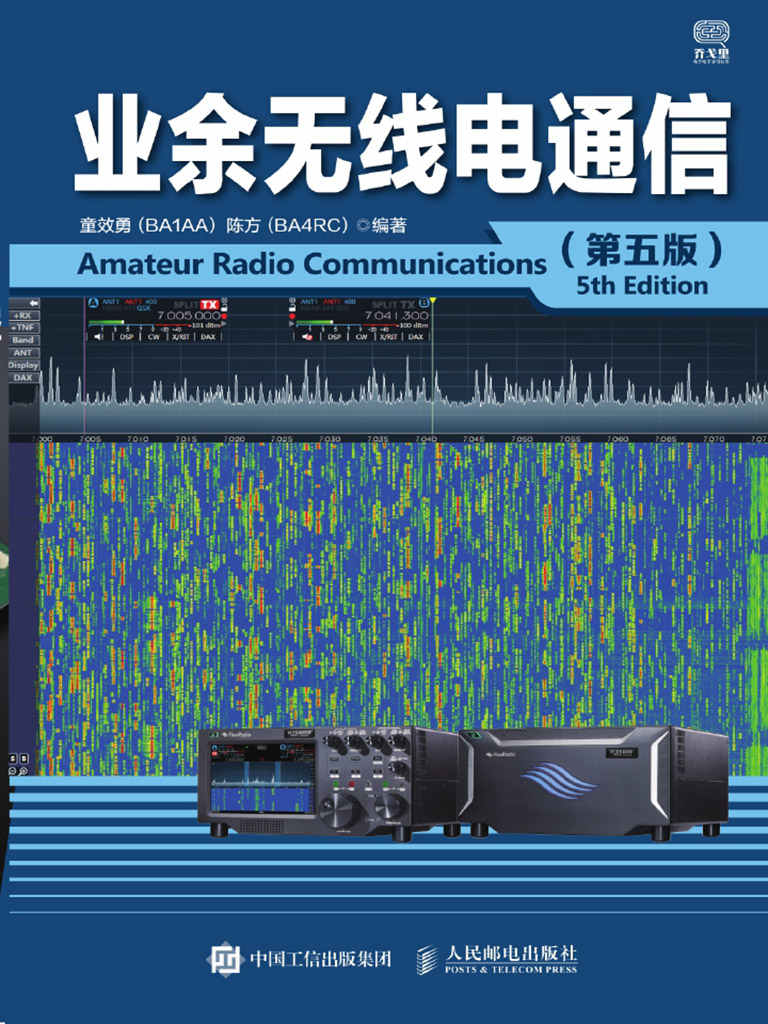
\includegraphics[width=0.7\linewidth]{cover}
	\caption{}
	\label{fig:1}
\end{figure}



\chapter{内容提要}

本书是由业余无线电家童效勇(BA1AA)和陈方(BA4RC)为广大业余无线电爱好者编写的业余无线电通信入门教材。

本书系统地介绍了开设、操作业余无线电台的相关知识和法律法规,主要内容包括:业余无线电通信简史、业余无线电通信操作实践、收发报技术的自我训练、业余无线电奖励证书和竞赛活动、不同业余无线电波段的运用、业余短波天线、业余无线电收发信机、依法设置和使用业余无线电台等。

本书既可作为开展业余无线电活动的教材,也可作为业余无线电爱好者的自修读本和手册。




\chapter{编著者的话}

业余爱好是人类社会进步的产物,是社会文明进步的标志。古今中外大凡发明创造者都有其业余爱好,而伟大的发明出自业余爱好者之手的例子更是不胜枚举。电气研究先驱者富兰克林12岁当印刷学徒并从未离开过印刷业;揭示电磁感应的法拉第也曾是报童、装订工,后来还成为一名化学专业研究者;电报机发明者莫尔斯发明电报时正从事大学的工艺美术教学……科学巨匠爱因斯坦说:“智慧并不产生于学历,而是来自对于知识的终生不懈的追求。”孔子也说:“知之者不如好之者,好之者不如乐之者。”不要被拜金主义、享乐主义和其他世俗的观点淹没了你的兴趣、爱好和激情!我们的祖国正需要千千万万个爱迪生式的发明家,而当今世界对人才的激烈竞争也正呼唤着每一个有志者从自己的业余爱好中去钻研、去实践、去塑造,以发现崭新的自我。

业余无线电通信活动以其极为丰富的内涵吸引了并将继续吸引着无数爱好者。科技性、先进性、实用性、群众性、国际性使这项活动与其他任何业余兴趣活动有着很大的不同;培养高素质的技术人才,丰富人们的文化生活,为抢险救灾提供有效的通信服务,促进各国人民间的交流,增进友谊,这一切正是改革开放不断深入的中国所迫切需要的。正因为这样,业余无线电通信活动及其标志—业余电台正越来越受到国家和各有关方面的重视,推动发展和加强管理的一系列法规、政策也已日趋完善。

我国有着大量的无线电技术爱好者,但进行业余无线电通信实践的人还不是很多。编写本书的目的是帮助更多的朋友学习和掌握业余无线电通信的基本知识和技能,尽可能地为乐于此道的爱好者们提供一本较为翔实的自我训练的教材。

改革开放的春风已吹绿了中国业余无线电通信芳草地,业余电台正如雨后春笋般出现在神州大地。愿爱好者在这里汲取更多的雨露和阳光,培育出更加绚丽夺目的奇葩—HAM之花!

1995年1月

\chapter{修订说明}

《业余无线电通信》一书自1995年出版以来,历经了数次改版、重印,2016年6月推出的第四版,也已陆续重印了三十余次。这说明在无线电技术和电子科学迅速发展的今天,这本“入门砖”性质的小册子,在广大业余无线电爱好者群体中还有一定的需求量。能够为我国业余无线电的发展尽一份微薄之力,这让我们感到十分欣慰。

为能适应科学技术和社会的快速发展以及业余无线电实践的丰富、进步,《业余无线电通信》先后于2004年、2011年和2015年进行过3次修订,出版了《业余无线电通信》第二版、第三版和第四版。在这几次修订中,除了对正文和附录里一些时效性较强的内容作必要的修改、调整外,改写了第8章《依法设置和使用业余电台》,增加了业余无线电在我国的发展简史,介绍了我国业余无线电爱好者群体在2008年汶川地震抢险救援应急通信工作中的突出表现,增加和改写了部分业余无线电通信操作实践方面的内容。

2020年10月,我们完成了《业余无线电通信》第4次修订。为能使书稿继续与时俱进,更好地服务于广大读者,我们在不改动原书总体结构的原则下,对涉及时效性的叙述及附录再次进行了修改调整,增加了软件无线电通信技术介绍、如何在线学习CW技术等方面的内容,在附录中增加了设计制作业余无线电测向机的相关内容。

《业余无线电通信》的每一次修订,都得到了许多业余无线电组织、业余无线电家和爱好者的帮助,在此一并向他们致谢。衷心感谢中国无线电运动协会,江苏、上海、天津等省、市无线电运动协会,中国无线电协会业余无线电分会以及龚万聪(BA1DU),陈平(BA1HAM),范斌(BA1RB),焦亮梅(BD1AYL),尹虎(BD1AZ),穆新宇(BD1ES),李彬(BA4REB),陈新宇(BA4RF),李家伟(BA4WI),卜宪之(BD4RG),姜锦中(BD4RQ),王龙(BD4RX),薛立人(BA5RX),郑英俊(BA5TX),陈衡(BD5RV/4),刘旭(BA8DX),刘虎(BG8AAS)等HAM在书稿校对、资料提供、翻译、新增内容的撰写等方面所给予的无私帮助,同时也感谢指正原书中的错漏之处并提出修改意见和建议的读者朋友们!

编著者

2020年10月22日

\mainmatter

无线电通信诞生于19世纪末。1888年,德国物理学家赫兹进行了一项著名的实验,他用火花隙激励一个环状天线,用另一个带缝隙的环状天线接收,证实了麦克斯韦关于电磁波存在的预言。赫兹实验激发了人们探索电磁波奥秘的热情,许多科学家都在努力研究如何利用电磁波传递信息,于是无线电技术蓬勃发展,人们的通信距离不断延伸。1901年,马可尼使用高功率的发射器首次完成了横跨大西洋的通信,揭开了无线电通信的新纪元。

20世纪初,无线电爱好者纷纷从事起无线电通信实验,商业电台数量迅速增加,电波干扰日益严重,各国政府都认识到需要制定一个法规,以保证频谱资源的合理分配和使用。1927年在华盛顿召开了世界无线电报大会,成立了国际无线电咨询委员会,并对广播、移动等各类无线电通信业务所用的频率进行了初次划分,将业余业务列入频率划分表,使业余无线电频率得到国际社会的确认。

业余无线电为无线电爱好者提供了一个广阔的舞台,无线电通信技术的发展同样也凝聚着全世界数百万业余无线电爱好者的智慧。短波通信、流星余迹通信、月面反射通信、无线电数字通信、无线电图像通信、低轨道卫星通信……业余无线电家们不断探索新的课题,在不到一百年的时间里,业余无线电从最初的无线电报逐渐发展成为利用计算机硬件、软件处理各种数字信号的全新技术。

\chapter{初识业余无线电}

从这个窗口看到的是整个世界。
——Carry V.Hammond VE3XN

1901年,马可尼成功实现了跨越大西洋的3200km距离的通信实验。1923年,业余无线电爱好者用小功率短波电台同样成功实现了横跨大西洋的通信实验。他们通过实验发现,波长越短通信距离越远,只需要较小的功率就能实现远距离通信。业余无线电爱好者的这一重大发现,是无线电发展史上最重要的成就之一,它为全球短波通信奠定了基础。

就无线电技术而言,业余无线电和其他无线电没有本质的区别。世界各国的业余无线电爱好者对无线电通信技术的发展起着重要的推动作用。在短波通信、流星余迹通信、单边带技术的研究与应用、月面反射通信、无线电数字通信、无线电图像通信、低轨道卫星通信等许多领域都留下了业余无线电家们不断探索的身影。在登山探险、抢险救灾、增进世界各国人民的友谊、培养青少年科技素质等方面,业余无线电通信也都展现了其独特的魅力和巨大潜力。

在科学技术迅速发展的今天,无线电通信已经深入到包括人们日常生活在内的各个领域。无论是天上的飞机、卫星,海上的轮船、舰艇,陆地上的各种车辆,还是人们熟悉的收音机、电视机、移动电话、Wi-Fi无线网络……全都离不开无线电通信技术。

业余无线电通信(以下有时简称“业余通信”)是整个无线电通信世界当中一个重要的组成部分。它是一项鼓励人们去从事无线电收信和发信实践的业余兴趣爱好活动。业余无线电通信的英语名字是“Amateur Radio”,符合国际电信联盟ITU定义的业余无线电爱好者是“Radio Amateur”,在世界上又普遍被称为“HAM”。由于“HAM”在英语中被解释为“火腿”,所以“火腿”又成了从事业余无线电通信的爱好者们的另一个名字。

业余无线电通信技术是一项内涵极其丰富的专门技术,所以人们还把获得发信执照、精通业余无线电技术和通信的爱好者称为“业余无线电家”,以区别于一般的电子技术爱好者。业余无线电通信的天地是博大的,当打开自己的收、发信机时,你可以听到来自世界各个角落的HAM的声音。当你获得业余无线电执照后,你可以轻松地和任何一个国家和地区的HAM交谈而无须办理出国护照,也可以从无数不见面的朋友那里得到技术上的支持。你会为自己第一次成功地和远方的朋友通信而兴高采烈,更可能会为自己在电子技术、通信技巧以及语言、人文地理等许多方面知识才能的迅速提高而大吃一惊!到那时,你才会更深切地体会到:业余无线电通信确实是一项遍及全世界的十分有意义的兴趣爱好活动。

\section{业余无线电通信的起源}

业余爱好者在无线电技术的发展和应用舞台上发挥了无可替代的重要作用。17世纪科学家麦克斯韦建立了完整的电磁场理论。1887年,德国物理学家赫兹第一次用实验证实了电磁波的存在。将这些科学成就应用到实践中,则首推业余无线电鼻祖意大利人马可尼。1895年,21岁的马可尼在意大利波伦亚他父母的别墅楼上与1.7km的附近山丘之间成功地进行了电报通信实验,他的这一业余科研成果使无线电通信成为现实。经过不断实验,1901年12月马可尼又成功地实现了电波横跨大西洋的实验。先驱们的行动激励了世界各地更多的业余无线电爱好者(Radio Amateur)去进行探索和研究,澳大利亚、英国和美国分别于1910年、1913年、1914年先后成立了业余无线电爱好者组织,爱好者的队伍日益壮大。

在商业和政府对无线电通信需求量大增的情况下,业余无线电通信被赶到了当时人们普遍认为没有实用价值的短波,爱好者们开始了新的试验。1921年,意大利罗马近郊发生了一场火灾,一台几十瓦功率的业余电台在短波段上发出了求救信号,结果却被远在千里之外的丹麦业余电台收听到了。1923年,美国的两位业余爱好者正在本土用短波相互联络,法国的一位业余爱好者意外地在欧洲听到了他们。于是,3人完成了这次具有历史意义的远距离通信。短波可以用于远距离的通信的事实引起了轰动,从此成为远程通信的主要波段,这也成为短波是业余无线电爱好者首先发现的经典证明和传颂故事。

业余无线电爱好者们执着不懈地涉猎各种未知的通信模式。20世纪50年代初期,美国空军发展新一代的轰炸机,在设计时去掉了报务员的位置,不用电报只用语音通信,但也带来了原有的调幅、调频通信难以满足距离的要求。贝尔实验室估计需要花费上亿美元的研究费用才能解决这个问题。但空军中的无线电爱好者莱曼和葛利斯伍德将军十年前就开始在自己的业余电台上试验“单边带”,这是一种效果比传统方式好得多的新技术。他们把自己的业余电台装到了一架飞机上,环球一周,始终保持了与位于美国内布拉斯加的司令部的联系。这种通信设备后来被无线电界广泛应用。

\section{中国业余无线电简史}

中国的业余无线电活动始于20世纪初至20世纪20年代初。西方先进科学技术的涌入和无线电广播业在华夏大地的萌动,激起国人对无线电技术的爱好与追求,他们从简单的矿石机收听起步,进而提高自己的收信水平直至发信,成为中国第一批业余无线电爱好者。如张让之(AC8ZT/XU8ZT/C1ZT)从光绪卅年(1904年)就迷上了电器机械,20世纪初,他又请友人从美国带回一套3灯机的材料,装成后昼夜收听CW(电报模式,见本章1.4.1),开始了业余无线电通信的研究。1930年他又开始研究短波发射,此后一直为我国业余无线电事业的发展贡献力量,直至1949年逝世。而供职于天津海关的蒋宗衡(X2AY/AC2AY/XU6AY),1923年就用X2AY的呼号开始了业余短波通信。

出现在中国最早的业余无线电组织是由在华的外国业余无线电爱好者于1929年成立的“中国国际业余无线电协会(The International Amateur Radio Association of China,IARAC)”。他们虽然在将业余无线电活动介绍到中国方面起到一定积极作用,但却无视我国主权,自定AC(Asia China的意思)呼号冠字、擅划中国业余分区。他们在业余界的霸道行为,引起国人的愤慨。

第一个由中国人建立的业余无线电组织为“中国业余无线电社(China Amateur Radio Union,简称CARU)”,系“中国无线电工程学校”校长方子卫(AC8FG)基于日本军国主义制造了震惊中外的“九·一八”事变而发起。方子卫于1931年10月在《新闻报》上呼吁我国业余无线电爱好者组织起来,效法欧美各国,平时进行科学实验,一旦国家需要即服务于国家。呼吁发出,得到爱好者的积极响应。1932年年初,CARU在上海正式成立,方子卫(AC8FG)任会长,由当时在无线电界有较大影响的张让之(AC8ZT)任副会长并进行实际运作。

CARU奉国际业余无线电爱好者遵循的6条规例为《业余无线电家之法典》,办有社刊《QSP无线电杂志Amateur Radio》,积极宣传业余无线电,努力引导爱好者开设业余电台。为抵制外人擅用的AC呼号和擅划的业余分区,CARU在国际分配给中国的字头中启用了XU为业余呼号冠字,划定了全国的业余分区,活动开展后又向政府主管部门提交了由正副会长签署的请愿书,要求政府颁布法规,使业余电台活动合法化,但未果,政府对业余无线电仍采取抑制态度。由于CARU是以无线电工程学校为依托的群众团体,发展的会员多为本校学员和周边地区及各地极少数积极分子,活动又得不到政府支持,所以到1935年年底后就逐渐淡出业余无线电界了。但这是我国第一个由中国人自己组织起来的业余无线电团体,在普及无线电知识与技术、振奋科学精神、团结和启蒙爱好者开展业余无线电活动方面起到了先锋作用。

CARU淡出后,全国各地仍有不少的业余无线电爱好者在进行业余通信。为把大家团结起来,争取政府对业余电台活动的认可,并以团体的力量来抗衡IARAC,1936年4月,杭州业余无线电家赵振德(XU8UX)发起成立“中国振中业余无线电研究社”(Chinese Calling Radio Club of China,CCRCC),同年11月更名为“中华业余无线电社”(China Radio Club,CRC)。

CCRCC-CRC是一个管理较为完善的团体,由各地爱好者代表组成了理事会,发起人赵振德(XU8UX)、济南黄小芹(XU3ST)分别被选为正、副社长,出版社刊《QSL》,建立全国QSL卡片管理系统,统一分配和管理社员呼号,重新划分业余分区,定期举办社员联谊会、技术讲座,组织竞赛活动、为抗日募捐等。不到一年时间,CRC社员及电台数量迅速增长,远远超过IARAC。一些大专院校也加入成为团体会员,大、中城市成立起分会、支会,在国际上也有了一定的影响。CRC也曾向政府提出申请,以便合法进行活动,但这种热情不仅未得到主管当局支持,反而在1937年5月被交通部下令解散。

而此时日寇侵华步伐加快,不久就在卢沟桥制造了七七事变,抗日战争全面爆发。业余无线电爱好者们更是义愤填膺,愤于报国无门,赵振德又先后与杭州、上海的原CRC理事、干事和积极分子多次协商,于1937年8月11日在上海交通大学召开了请愿大会,一致决议成立“中华业余无线电社非常时期服务部”,并于9月派出专人前往南京向政府提出申请。迫于当时国共合作、全国人民一致抗日的形势,申请很快获准,正式命名为“军事委员会第六部业余无线电人员战时服务团”,后更名为“军事委员会政治部业余无线电人员战时服务团”(以下简称“战时服务团”)。

“战时服务团”团长实为挂名,实际领导人为副团长朱其清(XU4KT/C1KT),隶属于郭沫若为厅长的第三厅,成立时间为1937年10月,从此业余电台活动得到了合法的地位。

“战时服务团”成立后,为抗日救亡做了大量工作,如向抗日游击队提供通信设备,为抗战培养无线电人才,侦察、干扰日伪电台,宣传抗战、揭露日寇罪行,坚持敌后联络等。有爱好者更是直接奔赴抗日前线参加战斗,如解放后曾任福建省冶金厅厅长的高振洋(XU7CK)等。

1940年5月5日,“战时服务团”创办了第一届空中年会,并将此日定为中国业余无线电节,每年举办一次,1949年后虽有中断,但自海峡两岸相继恢复业余电台活动后,又开始并延续至今,为爱好者相互交流、向社会宣传业余无线电活动提供了一个极好的平台。

1940年9月,“战时服务团”转名为“中国业余无线电协会(Chinese Amateur Radio League,CARL)”,获准在社会部登记备案,原来的正副团长改为正副会长,实际负责人仍为副会长朱其清。

CARL有完整的协会章程、会徽、会歌、会员证、广播电台,并根据抗战胜利后国民政府重新划分的行政区域,划分了业余无线电分区,决定全国业余电台统一使用“C”为呼号冠字,印制了业余电台执照,制定了电台设台手续和管理规定,颁布分会、支会组织法,完善了协会各级组织,出版会刊《CQ协刊》和《无线电世界》,还面向社会举办无线电讲座,积极参加公益活动,为国民政府第七届全运会提供通信服务等。同时,CARL积极介入国际交往,1947年加入“国际业余无线电联盟”(IARU),朱其清还作为业余无线电界的代表参加中国代表团出席1947年在美国大西洋城召开的国际电联(ITU)大会,到会后又被聘为“国际业余无线电联盟”(IARU)代表。到1949年,CARL会员数量已逾5000,电台超过400部。

朱其清在上海解放一个月后,代表CARL召开各界代表座谈会,探讨业余无线电如何为新中国服务,上海分会还专门在原爱多亚路的南京大戏院西邻租房办公,发展会员、举办讲座、出版刊物、号召爱好者为新中国出力。一些地方分会的爱好者为了迎接解放,保卫新生政权,在保护设备免受破坏、剿匪、监视国民党残余势力活动、宣传新中国等方面都做出了很大贡献。可以说,CARL时期是解放前我国业余无线电活动发展的鼎盛时期。

纵观民国时期的业余无线电活动,从CARU开始到CCRCC-CRC再到“战时服务团”CARL,这些由国人组织起来的业余无线电团体及其创始人、组织领导者和许多老业余无线电家们,在中国业余无线电发展历程中,做出了不可磨灭的贡献。他们在逆境中奋进,热爱科学、热爱国家,勇于奉献的精神,为后人留下了一笔可贵的财富。

中华人民共和国成立之初,鉴于形势需要,业余电台及其相关的活动被全部禁止。1952年,根据刘少奇同志的建议,开始在全国范围开展“国防体育”活动,以便向军队输送技术兵和作为国防后备资源。无线电作为“国防体育”的一个项目,在各地“国防体育协会”下属的“无线电俱乐部”领导下有组织、有计划地在群众中尤其是青少年中被广泛开展了起来。

1958年,“国防体育”合并到体委系统,各项活动改由各级体委组织管理。原来这些科技含量较大的项目,融入了更多的体育比赛内涵。当时无线电活动开展的项目为工程制作和报务(即抄收和拍发电报)两项,主要在全国各地的大、中、小学和青少年科技活动场所开展。20世纪60年代初,又增设了无线电通信多项和无线电测向两个项目。

为便于对外交往,1964年中国无线电运动协会(Chinese Radio Sports Association,CRSA)成立,隶属于体育总会,不发展个人会员。

业余电台的恢复得益于1958年在北京举办的“国际快速收发报竞赛”。保加利亚代表团团长报到后随即建议设立业余电台供参赛各国有执照的爱好者联络,组委会采纳了这一提案,并由竞赛总裁判长、原邮电部党组书记、中国人民解放军通信兵部部长王诤亲自负责,建立了中华人民共和国的第一个业余电台,并亲自命名呼号为BY1PK(寓意中国第一个业余电台在北京),结束了祖国大陆自1949年以来没有业余发信的历史。该电台限用CW且只能与当时的社会主义国家联络。1963年后,北京、长春、西安、长沙、成都各建起一座集体业余电台。

1975年,军事体育(即原“国防体育”)在全国恢复,无线电活动也逐步开展起来。

随着改革开放的春风,众多老业余无线电家积极呼吁恢复业余电台,全国人民代表大会代表老业余无线电家周海婴(BA1CY)还向全国人大提交了提案,外国业余无线电爱好者或团体也通过各种渠道希望中国开放业余电台。

1981年6月,我国无线电通信界的老前辈,原电子工业部副部长、中国电子学会理事长孙俊人院士,在北京召集有关部门领导和部分老业余无线电家、无线电及电子行业的老专家开座谈会,大家一致认为应该尽快恢复业余电台活动。根据会议精神,国家体委于同年11月向国务院上报了《关于恢复开展业余电台活动的请示》,获准首先恢复集体业余电台活动。关闭了16年之久的BY1PK终于在1982年3月恢复发信,并且取消了只准联络社会主义国家的限制,不久又取消了只能使用CW操作的规定。同年国家无委、国家体委联合颁布《业余无线电台管理暂行规定》,用法规形式确定了开展业余电台活动的积极意义。

20世纪80年代和90年代初期,集体业余电台在全国得到迅速发展,各地有条件的体委系统以及很多大、中学校和青少年教育基地,乃至有些小学和工商企业都先后建台,分布范围达20多个省份和全国10个业余分区。

1984年6月我国在“国际业余无线电联盟”(IARU)的席位得到恢复。这一时期集体业余电台的活动,在普及科技知识、拓宽爱好者尤其是青少年的知识领域、丰富人们文化生活、宣传业余电台活动以及加强国际交流等方面,都起到了积极的作用,同时,也为业余电台活动积累了管理经验,为恢复开放个人业余电台打下了基础。

随着改革开放的不断深化,人民生活水平不断提高,爱好者们要求恢复开放个人业余电台的呼声不断增长。1992年3月16日,老部长孙俊人再次邀请主管部门领导、老业余无线电家和有关方面负责人,就进一步发展我国业余无线电台活动,恢复开放个人电台问题进行研讨,大家一致认为,应加快步伐,尽快恢复开放个人业余电台,以适应国内外形势发展的需要。会后国家无委办公室根据会议精神和有关领导的指示,于4月22日向国家无委主任朱镕基副总理提交了“关于进一步开放业余无线电台的请示”,很快获得批准。根据批示,国家无委和国家体委共同制定了《个人业余无线电台管理暂行办法》,并于1992年8月14日正式颁布。

1992年12月22日,第一批20多名老业余无线电家的个人业余电台正式发信。不久又开始在全国范围进行了“个人业余电台操作证书”考试,取得证书的爱好者纷纷建台。从此大批爱好者,尤其是青年爱好者源源不断地加入,业余无线电人数迅速增加。到2012年年底,我国内地业余电台数量已逾十万,并几乎涉足于世界业余无线电领域的所有项目。由我国爱好者自行设计、参与制造的业余卫星“希望一号”,于2009年12月15日搭载“长征四号丙”运载火箭成功升空,填补了我国在这一领域的空白。在各种突发自然灾害和紧急救援中,业余无线电爱好者们做出了积极的贡献,社会对业余无线电的认知度不断提高。

工业和信息化部于2012年年底颁布《业余无线电台管理办法》。2013年2月,工信部发布《关于实施〈业余无线电台管理办法〉若干事项的通知》。新法规理顺了管理体制,简化了设台的审批手续,方便了爱好者们对无线电技术的探索、研究和各类活动的开展,体现了国家对业余无线电更加开放、更加人性化的政策,为更加有序、迅速的发展提供了保证。

\section{我国业余无线电爱好者在突发事件中的几个真实故事}

业余无线电在突发事件中的积极作用,早已被世界各国所公认,近年来如1995年日本神户大地震、2001年美国的9·11事件以及2004年的东南亚大海啸中都有业余无线电爱好者们做出贡献的事迹。随着我国业余无线电活动的深入发展,中国业余电台和业余无线电爱好者们也创下了许多可圈可点的业绩。

1988年5月5日,中国、日本、尼泊尔三国联合登山队,分别从南北两侧攀登世界第一高峰—珠穆朗玛峰,成功地实现了两支队伍在顶峰会师并分别从另一侧顺利下撤的“双跨”壮举,在世界登山史上写下了辉煌的一页。然而在登顶、会师过程中,当北侧的中方队员第一个登上顶峰后,却迟迟不见南侧队员到达。已在高寒缺氧的顶峰创纪录地不用氧停留了80min的中方队员,还要不要继续等待下去,必须由北京总指挥部决策。而此时的主峰,云雾缭绕气候变化莫测,盘旋在上空的侦察飞机也无能为力。设在大本营的业余电台BT0 ZML将顶峰及两侧队员的情况,通过拉萨业余电台BT0LS及时传到CRSA的集体台BY1PK,使前线的情况及时到达总指挥部,指挥部的决策命令又从同样的路径返回传达到了登顶队员的耳中,这一“路径”一直保持到会师、下撤。5月8日23点50分,由于天气迅速变坏,北侧大本营三国指挥员对是否还要进行第2次、第3次突击顶峰产生了严重的意见分歧,必须请示北京总指挥部做出最后决策。可是通信网的约定联络时间已过,北侧大本营业余电台操作员想到了世界各地随时都会有爱好者活跃于业余频段上,他立即发出“普遍呼叫”(见第2章2.7.2)。求助信号被一位日本爱好者听到了。这位爱好者马上从东京通过长途电话唤醒了在北京的总指挥。零点刚过,北京的业余电台即开机发信,传达了总指挥部的决策命令,圆满解决了难题。

1991年夏,洪水肆虐苏南大地。6月的一天,江苏省无线电运动协会业余电台(BY4RSA)的爱好者正在进行对外联络,一位澳大利亚业余电台着急地要求通话,原来操作者是该国业余救灾通信网的主任。他说,他们那里的爱好者已经做好准备,要为中国灾区募集医药物资,要组织医疗队到中国来。江苏的爱好者立即和有关方面取得联系,并和澳大利亚业余救灾网保持了不间断的联络。不久,美国的业余救灾网也加入进来。经过爱好者们的努力,10多吨医疗物资分别从澳大利亚、新西兰、美国送到了江苏灾区。

2008年5月12日,四川汶川发生特大地震,业余无线电通信以其台站数量大、分布范围广、爱好者技术全面勇于奉献等优势,在抢险救灾中做出了突出的贡献。地震发生后不到3min,成都的业余无线电应急通信网启动并开始呼叫,立即得到省内外的大量HAM响应,十几分钟内,就从各地爱好者的报告中得知震中及省内其他所有震区的位置,还和有业余电台的震区取得了联系,并得知汶川及很多重灾区的正常通信已全部中断,于是又立即动员了省内外爱好者携带设备进入震区和交通中断的地区。经无线电管理局同意,13日四川省业余无线电应急通信网指挥中心组成,以BY8AA作为主控台呼号,纳入省抗震救灾指挥系统,对所有参加四川救灾的业余电台进行统一指挥、调度。在正常的通信系统恢复前,业余无线电应急通信网成为抗震救灾指挥通信的主要渠道。为了尽快恢复各地的通信,13—14日,各大无线通信设备经销商、运营商和信息产业局等有关单位全部出动,但是技术人员出现很大缺口,指挥中心又从省内外调集了多批技术全面的爱好者前往支援。各种专业通信网建立后,业余无线电爱好者们的主要工作又转向了为志愿者的行动及救援物资调度等提供通信服务。到5月17日,电台值班联络日志上的记录就有300多页,仅在日志上出现的HAM就有1900多名。投入各类通信设备超过6000台套,参与调动车辆8000余台次,转运伤员近万名,以上仅是短短6天的不完全统计。“生命救援”阶段结束后,业余无线电爱好者继续为后续救助提供服务,依托迅速有效的通信手段,形成了规模最大、效率最高的民间志愿者调度枢纽。HAM们在抗震救灾期间的突出表现,受到了当地政府、无线电管理机构、商业无线电部门以及民众的一致赞扬,美国无线电转播联盟ARRL也将《2008年人道主义奖》授予了四川抗震救灾的业余无线电爱好者们。

\section{独特的业余电台}

联合国下设的专业机构“国际电信联盟”(ITU,International Telecommunication Union)根据不同的用途将全世界所有无线电通信分为若干种“业务”(Service),其中有两种业务用于业余无线电(Amateur Radio):“业余业务”(Amateur Service)和“卫星业余业务”(Amateur-Satellite Service)。ITU对业余业务的定义为“供业余无线电爱好者进行自我训练、相互通信和技术研究的无线电通信业务。业余无线电爱好者系指经正式批准的、对无线电技术有兴趣的人,其兴趣纯系个人爱好而不涉及谋取利润”。对卫星业余业务的定义是:“利用地球卫星上的空间电台开展的与业余业务相同目的的无线电通信业务。”用于业余业务的电台称业余电台(Amateur Radio Station)。业余电台是经过国家主管部门正式批准,业余无线电爱好者为了试验收发信设备、进行技术探讨、通信训练和比赛而设立的电台。

根据设台者的身份,业余电台可分为个人设置和团体(单位)设置两种。根据电台核准使用的频率和发射功率,我国又将业余电台分为A、B、C三类,以及特殊业余电台。只收听而不发射的电台被称为收听台,简称“SWL”(Short Wave Listener)。SWL虽然不发出信号,但它同样可以体会到HAM世界的美妙风光,帮助你和其他爱好者取得联系,而不用担心在稠密的住宅群中因为你的发信干扰了邻居的电视而招来不快。世界上有许多收听爱好者。

由团体(单位)申请设置的业余电台常被称为俱乐部电台(Club Station),我国曾于2013年前将这种电台定义为“集体业余电台”,并曾规定这类电台的呼号前缀(见本章1.3.3)为“BY”。这些“BY电台”多为学校、各类校外青少年教育机构、协会所设立,曾经为普及业余无线电知识、增进青少年爱好者对无线电科技爱好的兴趣发挥了积极作用。目前,仍有不少BY电台活跃着。现在,俱乐部电台和个人电台的呼号前缀已不做区分。本书附录3记录了部分BY电台的呼号,以便于了解这段历史和作为备查的资料。
个人业余电台是指爱好者本人申请设置并由其本人操作使用的电台。当今世界200多万个业余电台中,绝大多数是个人台。
在任何国家、任何地方,未经国家主管部门批准的无线电发信(包括试验发信)都是被严格禁止的。

你可能很想参加业余无线电通信活动,急于了解一系列的问题,比如:

\begin{itemize}
	\item 什么是业余电台?
	\item 业余电台可以进行哪些通信实验?
	\item 业余电台能通联多远?
	\item 我能够玩转业余电台吗?
\end{itemize}  

\subsection{“火腿”与业余电台}

这里所说的“火腿”不是“金华火腿”,它特指对业余无线电通信有着浓厚兴趣的人。业余无线电爱好者的英文是“Radio Amateur”,又称为“HAM”。由于“HAM”在英语中还可以被解释为“火腿”(见图1-1),所以“火腿”又成了业余无线电通信爱好者们的另一个名字。

\begin{figure}[htbp]
	\centering
	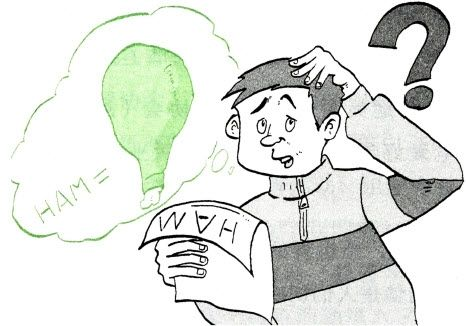
\includegraphics[width=0.7\linewidth]{1}
	\caption{业余无线电通信爱好者}
	\label{fig:1}
\end{figure}

业余无线电台(Amateur Radio Station)是经过国家无线电主管部门正式批准,业余无线电爱好者为了试验收发信设备,进行技术探讨、通信训练和比赛而设立的电台。业余电台中的“业余”一词,并不表示从事业余无线电通信活动的人缺少专业知识与技能,而是强调业余无线电不能用于商业目的。国际电信联盟(ITU)根据不同的用途将全世界所有无线电通信分为43种业务,业余电台属于其中的“业余业务”。ITU对业余业务的定义为“供业余无线电爱好者进行自我训练、相互通信和技术研究的无线电通信业务。业余无线电爱好者系指经正式批准的、对无线电技术有兴趣的人,其兴趣纯系个人爱好而不涉及谋取利润”。

世界各国政府对业余无线电活动都给予了多方面的支持,允许无线电爱好者通过无线电波跨越国界进行国际间的交流,因此业余无线电爱好者也被称为各国的民间友谊大使。目前全世界拥有电台呼号的爱好者约300万人,如果你拥有了自己的电台和呼号,成为“火腿族”的一员,你就可以和国内外的业余无线电爱好者进行空中对话了。

下面摘录的是美国业余无线电协会(ARRL)出版的《业余无线电爱好者手册》中一段有关业余无线电通信的说明。

“一年365天,全世界的业余无线电爱好者都随时相互进行着通信。通信是人们切磋有趣的技术,进行富于变化的、激动人心的试验,发现新朋友的手段。业余无线电家作为具有共同的广泛兴趣的人们,通过全球规模的‘友谊之桥’,进行空中通信,交换思考的话题,互相学习。因此,业余无线电通信具有超越国界、增强理解和友谊的作用。这一点是其他爱好所无法实现的”。

\subsection{集体电台和个人电台}

根据设台者的身份,业余电台分为集体电台和个人电台两种。由团体申请设置,并由设台团体使用的称为集体业余电台,国际上常称其为俱乐部台(Club Station)。我国现有的集体业余电台,多为体育、教育、科协等系统所设立,是组织、培训爱好者的活动中心。个人业余电台是指爱好者本人申请设置并由其本人操作使用的电台。当今世界300万个业余电台中,绝大多数是个人电台。

中国的业余无线电活动开始于20世纪20年代,在当时极其简陋的条件下,老一辈业余无线电家怀着“以科学报效祖国”的理想,自己动手制作无线电收、发报机,互相联络,成为掌握无线电通信技术的先锋。新中国成立后,党和国家领导人十分重视在青少年中开展无线电活动,参照前苏联建立“陆海空志愿协会”军事后备组织的模式,我国建立了中国人民无线电俱乐部等机构,陆续从东欧引进快速收/发报、无线电测向、无线电多项通信等活动,组建专业运动队参加国际比赛。1958年在北京建立了我国第一座集体业余电台BY1PK。1992年,经国务院批准,我国恢复开放个人业余电台。从此,我国的业余无线电活动进入了一个新的阶段。近年来,随着中国经济的飞速发展和世界范围内文化交流的加强,业余无线电已揭开它神秘的面纱,逐步成为许多爱好者业余生活的重要内容,如图1-2所示。各地的业余无线电爱好者积极加入到普及通信知识和操作技能的活动中,时刻准备在突发灾害到来时为社会服务。还有的爱好者正在进行数据通信、空间通信等各种新技术的研究。

\begin{figure}[htbp]
	\centering
	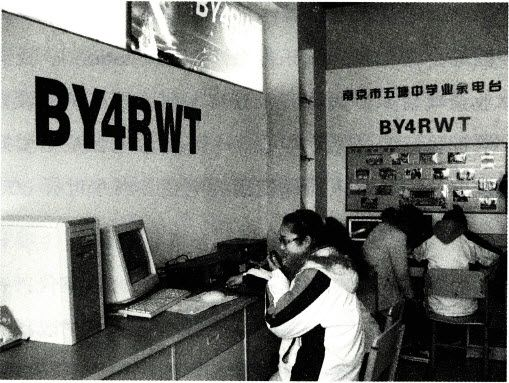
\includegraphics[width=0.7\linewidth]{2}
	\caption{业余电台BY4RWT}
	\label{fig:1}
\end{figure}

\section{业余无线电活动}

业余无线电爱好者进行通信实验的内容是极其丰富的,既有“古老”的电报通信,也有各种各样的数据通信和图像通信。世界各国的爱好者还把电台设备带到野外相互通联,进行移动通信、小功率通信实验。捕捉“突发E层”、“大气波导”进行VHF/UHF波段超远程通信试验是最具魅力的研究课题之一,将互联网与电台结合在一起的Ecohlink同样也吸引着众多的业余无线电爱好者。

业余电台活动包括了广泛的内容,如以提高操作技能为主的通信实践,以科研创新为目的的各种研究试验,以自力更生研制设备、提高动手能力为目的的各种工程制作,各国爱好者之间人员、信件频繁往来的友好交往等。而这些活动所需要的基础,如电子、物理、通信、计算机技术,以及外语、地理知识乃至爱好者个人的品德素养,又促使爱好者不断地学习和提高。
1.4.1 多种多样的通信操作实践
业余电台通信是和世界科学技术同步发展的。在无数次相互联络中,人们使用各种方式进行无线电通信的操作实践,并称之为“ON AIR”。常见的通信方式有以下两种。
(1)语言通信。根据语音信号对载频调制的不同方式,可分为调频话、调幅话和单边带话等。前两种发射效率较低、占用频带宽,一般限于在超短波、小功率下运用。在短波(HF)段一般都采用占用频带较窄的单边带话,简称SSB方式(Single Side Band)。在通信中,双方直接利用语言,主要是英语明语以及“通信用Q简语”和缩语(详见第2章)交谈。由于这种方式的操作比较容易,所以虽然所需设备比较复杂,但仍深受广大爱好者尤其是初学者的青睐。
(2)等幅电报通信,简称CW方式(Continuous Wave)。这种通信方式有着悠久的历史。它通过电键控制发信机产生短信号“.”(点)和长信号“—”(划),并利用其不同组合表示不同的字符,从而组成单词和句子。CW方式所需设备最为简单、占用频带很窄而发射效率较高,在同等条件下通信距离更远。而且,CW语言是一种真正的“世界语”,学习CW技术基本不受爱好者原有文化程度影响,所以虽然其技术“古老”,但在业余通信中仍占有重要的位置,资深爱好者的熟练技巧也往往在CW中得以淋漓尽致地发挥。和许多国家一样,我国也把CW技术作为爱好者取得发信资格的必要条件之一。现在,由于手机的普及以及电子电键、计算机的出现,爱好者自学CW技术已非难事,如果每天坚持利用闲暇时间保持一定的练习,数月之内达到可以上机操作的水平是完全可能的。
1.4.2 各种数据通信研究
随着计算机技术的普及,数据通信的研究水平也越来越高。
1.无线电传,简称RTTY(Radioteletype)
无线电传是一种对设备要求较低的数据通信,它用“移频键控”(FSK)的方式发射,即用键盘操作,发出的信号以不同的频率表示“1”或“0”,用若干个“1”和“0”的不同组合代表不同的字符。RTTY常用2125Hz代表“1”(亦称“记号”或Mark),2295Hz代表“0”(亦称“空号”或Space),也有以1275Hz代表“1”、1445Hz代表“0”的,然后再用这两种频率的信号去调制高频信号。发射出去的信号则是两个高频——高频的基本频率与上述两个音频之差。
在进行RTTY操作时,调制解调器把由键盘操作产生的字符信息转换成由两个不同频率信号组成的“五位码”(Baudot),再用这些表示数据“0”或“1”的一串串音频信号通过单边带方式调制并发射出去。接收端把这些信号还原成字符并在监视器屏幕上显示出来。收发双方轮流操作,可以进行“空中笔谈”。我国的青少年爱好者曾利用“娃娃电脑”和一台黑白电视机加上他们自己制作的简单调制解调器成功地进行了RTTY通信试验,上海的爱好者还编出了用计算机直接进行RTTY操作的软件。由于空间存在各种干扰电磁波,接收RTTY时屏幕上有可能会出现许多莫名其妙的字符,所以进行远距离RTTY试验时要有充分的耐心。在发射RTTY信号时,发信机将处于持续输出大功率状态,这对发信机的安全是很不利的。为保护发信机,应事先降低输出功率,采用“半功率”输出,而且不允许长时间不间断发信,这是RTTY初试者必须牢记的。
2.AMTOR方式通信(Amateur Teleprintion Over Radio)
这是一种具有纠错码功能的电传通信方式。它的原理是把RTTY代码转换成“7单元恒比码”。这种代码的特征是,组成每个字符的7位数据总是包含4个“0”和3个“1”。接收台就利用这个特征,自动检测收到的信息中“0”和“1”是否保持4∶3的比例,如果符合就认为是正确的,如不符合,接收台就自动做出相应的反应。当人们在进行AMTOR键盘操作时,计算机把信息编为3个字符一组,每发出一组,电台便有一暂停,由接收台自动应答。这个应答包含一个字符,表示刚才接收的一组信息是否正确,再由发信台自动确定继续发下一组还是重复前一组信息。
AMTOR的速率为100Baud。这种方式的抗干扰能力比较强,在信号很弱的情况下也能保持正确无误,而且每发一组信息仅210ms左右,可以不用担心发信时间过长的问题。你可以细心搜索一下收听频率,如果听到一种短促的像两只蟋蟀轮流振翅鸣叫一样的声音,那便是AMTOR信号。
3.业余无线电分组数据交换通信(Packet Radio)
前面两种数传方式都是把字符信息一个接一个顺序向外发射,即所谓“实时信息交换”,而且需要双方都有人在机上操作,如果你停止键盘操作,信息也会停止发送。Packet则不同,计算机以及专用的终端控制器TNC(Terminal Nod Controller)自动将要传输的内容分成若干段,并在每一段的头尾加上接收端地址和发送端地址等信息,形成一个个“数据包”,由电台发射出去。接收端对数据包检测并发出应答信息,要求发射端重复或继续发送下一组数据。用这种方法,你可以将事先存入计算机的信件文章或程序软件、图像文件准确无误地发出去。操作者不用去关心这些信息是不是按顺序发的,接收方计算机会自动接收,正确辨认,并且可以自动存盘而不必有人守候;双方也可以通过键盘“笔谈”。
与前两种方式不同,在Packet方式下你不必等对方“讲”完一句再回答,双方可以同时进行,计算机会自动把收、发内容分别显示出来。世界上有许多爱好者运用Packet技术组成了数据交换网、中继网,我们可以从这些网内的计算机里获取许多有关业余无线电的信息,也可以把自己的信息迅速传送到世界任何地方。
我们在HF段常用的Packet信号调制方式类似于RTTY,在电台里听起来好像吹哨子的声音,传送速率一般为300Baud。在超短波用“调频”方式传送,速率可达1200Baud。另外还有一种用“相位调制”方法工作的Packet,在短波传送的速率就可达1200Baud。
世界上有许多爱好者把自己的设备义务贡献出来,组成了国际业余计算机无线电通信网络。我们可以在14.101MHz、14.111MHz或21.101MHz和21.111MHz用“下边带”方式听到这些电台的信号。任何一个爱好者都可以把自己的计算机和这些网联系起来,从中读取各种有关业余无线电的资料信息。如果取得了相应的发射许可,也可以把自己的信息提供给大家或是由这些网络自动转发到你指定的地方。
4.APRS自动位置报告系统
当全球定位系统给人们带来极大方便时,许多HAM便开始了APRS试验。APRS是英语“自动位置报告系统”(Automatic Position Reporting System)的缩写。全球定位系统可以让你了解自己所在位置,而APRS则是通过无线电把全球定位系统数据发射出去,让别人知道你在什么地方。
1992年,美国爱好者Bob(WB4APR)首创了APRS系统。1999年,APRS开始接入互联网,爱好者可以通过因特网把自己的位置信息发布到遥远的地方。
移动APRS系统由一个全球定位系统加上一个被称为TT的控制转换电路和一部电台组成。TT电路把全球定位系统的定位数据转换成音频数字信号并控制业余电台加以发射。把接收端电台收到的信号输入计算机声卡,经软件解调后便在电子地图上显示出发射台所在位置及其移动轨迹的详细信息。现在,这项技术已经商业化,许多厂商在产品电台里嵌入了APRS模块,自动位置报告系统在社会许多领域里发挥出重要作用。
5.极弱信号数据通信实验
随着计算机科学的发展和数字信号处理技术(DSP,Digital signal processing)日臻成熟,使得在极弱信号条件下进行可靠的无线电通信成为可能。
月面反射通信(EME)是爱好者从20世纪40年代就开始的极弱信号无线电通信实验之一。由于传播路径长、月球表面粗糙且不规则,虽然发射功率有数百瓦或更大,但收到的反射信号依然十分微弱,用模拟信号如SSB语音或CW电报方式实现EME十分困难。直至出现了基于DSP技术、对所交换的信息具有自动侦测、重复、纠错和解码功能的通信协议程序(通信模式),才使更多的爱好者使用普通的设备以更高的频率完成了EME实验。
最著名的极弱信号数据通信模式当属JT65。该协议程序由天体物理学家、诺贝尔物理学奖获得者Joe Taylor(K1JT)编写,多用于进行EME、高速流星散射等通信实验。近些年来,爱好者将这种模式用于地面上的QRP小功率或恶劣传播条件下的DX远距离通信实验,获得了“意外的惊喜”,许多面向微弱信号条件的通信模式应运而生。常见的有FT4、FT8、JT4、JT9、JT65、QRA64、ISCAT、MSK144和WSPR,以及称为Echo的通信协议等。在这些通信模式当中,最受欢迎的当属FT8。

FT8由K1JT(Joe Taylor)和K9AN(Steve Franke)创建,使用8频率FSK(移频键控)方式调制,具有FEC自动纠错功能,解码阈值为-20dB,在极弱信号远距离通信中表现突出。
FT8受到世界各国爱好者追捧的原因还在于它具有自动、半自动的操作方式。所谓自动方式,是指FT8在主动呼叫CQ的状态下,具有自主发出呼叫信息并检测是否有应答信号,如有应答,便自动回复,完成QSO通联并自动保存通联记录,如没有应答或未能解析出有效应答信息,则继续发出CQ呼叫,整个过程全部自动完成。
半自动方式是指FT8在监测状态下可自动识别频率上正在以这种模式发出呼叫CQ的信息,如果你想回复这些电台,就可以在其完成一次呼叫后立即手动操作发出自动生成的应答信号,如果收到正确的回复信息,这次QSO便可得以完成。
目前最常用的操作FT8模式的通信软件是WSJT-X。这是一款免费、开源软件,适用于前文所述的多种极弱信号数据通信模式,其当下最新版本WSJT-X 2.2.2,以及软件使用手册、开源代码等,均可从相关网站下载。
WSJT-X已经推出简/繁体中文版本,增加了和常用比赛通联日志(如N1MM)关联功能,使爱好者可以非常方便地进行FT8模式DX通信联络和参加国际比赛。爱好者还编写出了远程控制操作电台程序,通过这种外挂的第三方软件,在异地或移动中,监控、操作家里的计算机和电台,非常轻松地用FT8模式自动实现了与人耳无法分辨的极弱信号DX电台的通信联络。当然,在用这种“机器人操作”方式工作时,电台的收/发信时间是1比1,且发射信号是恒定包络的连续波,对于电台及其电源的散热、安全以及对电磁环境可能造成的负面影响都是不可忽略的问题,而且这种由机器人代劳完成的通联也少了几分战胜困难提升技艺的乐趣。
1.4.3 各种图像通信研究
图像业余通信的发展反映了现代通信技术的突飞猛进,更体现着HAM执着的追求。目前常见的图像业余通信方式有以下几种。
(1)无线电传真(FAX,Facsimile)。发送端的传真机通过光电转换将文稿图片的黑白信息变成电信号发射出去,接收端再将电信号转换成光电信号,从传真机上便可以得到原稿真迹了。
(2)业余电视(ATV,Amateur Television)。在业余波段上传送HAM自己的电视是十分有趣的尝试。1987年在上海举办的全国运动会赛艇比赛中,起点的观众就是通过上海市业余电台的业余电视观看众多选手终点冲刺情形的。在我国无线电测向比赛中也多次进行过ATV试验。但是,ATV在业余微波频段传播距离有限,目前还没有大范围的业余电视转播网出现。
(3)慢扫描电视(SSTV,Slow Scan Television)。普通电视为保证其清晰、动作逼真,每秒须传送50幅图像(隔行扫描),要占用6MHz宽的频带。业余频段范围比较窄,难以传送一般的电视信号。爱好者们采用几秒传送一幅图像的办法,用图像信号的慢变化来减少所占频带的宽度,使在短波波段传送图像的愿望得以实现。SSTV方式把画面的明暗转换成不同的频率信号,再用以调制射频并发射出去。因为接收一帧完整的画面要好几秒,以前SSTV的接收端总是用中长余辉显像管做显示器以减小图像的闪烁感。现在,许多爱好者借助于计算机技术,使彩色图像的传递试验也获得了成功。
慢扫描电视的标准是:

\begin{figure}[htbp]
	\centering
	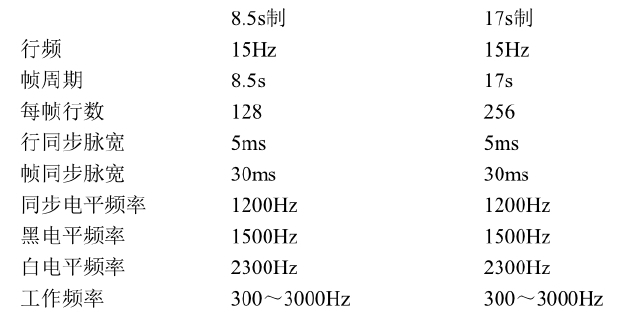
\includegraphics[width=0.7\linewidth]{86}
	\caption{}
	\label{fig:1}
\end{figure}

1.4.4 业余无线电卫星通信
1.业余无线电卫星简史
业余无线电卫星的研究与世界其他卫星工程的起步在时间上相差不多。1958年1月至5月,苏联的卫星sputnik和美国的探索者一号相继升空。与此同时,美国的一些爱好者萌生了发射业余无线电通信卫星的设想。他们组织起来并将这个计划命名为OSCAR(Orbiting Satellite Carrying Amateur Radio),目标就是制造和发射业余无线电通信卫星。4年之后,他们的努力获得成功,世界上第一颗业余通信卫星OSCAR-1号在美国加利福尼亚的范登堡空军基地由发现者36号火箭携带升空。
历经了几十年的探索,现在的OSCAR卫星,在技术上有了重大进步。但在开发过程中,爱好者的“业余”传统一直延续了下来,并体现在最新的卫星设计上。比如OSCAR-13,这是一颗AMSAT Phase 3卫星,其中大部分子系统是自制的,有些部件甚至是从二手市场上购买的。卫星内部连接各模块的玻璃纤维杆是在AMSAT(业余卫星组织)一位副主席家厨房里的炉子上加工的;用于制造导热毯的材料来自捐赠,由一位志愿者在他家地下室里用手缝制而成。另外一个业余通信卫星Phase 3-D的很多部件用的也都是类似的“廉价”的制作手段。比如,用以展开和固定太阳能电池组的装置,实际上跟普通门闩的结构没什么两样。卫星构架用的是普通铝片,许多天线用的也是一般材料,加速发动机和电池用的则是一些废旧边角料,其中很多材料是各国航天公司捐赠或从他们那里低价购得的。
尽管业余卫星制作成本低廉,但其精致程度足以与运营中的商业卫星相媲美。自20世纪80年代以来发射的业余卫星已具相当水平。根据国际业余卫星组织网站AMSAT资料显示,目前在轨运行的业余无线电通信卫星约有40多颗,有些星携带有BBS系统,爱好者可以9600bit/s的速率与之连接并使用它。利用现在的业余无线电数据分组通信卫星(PACSAT)所组成的网络,理论上爱好者们可以在地球上任意两地收、发信息,而这一过程只需几秒。业余卫星的语音转发器使得爱好者可以有更多的操作模式选择,从CW到SSB再到FM。有些卫星还允许地面上的电台之间通过它进行业余电视(FSTV)或慢扫描电视(SSTV)的通联。更重要的是,业余爱好者作为开拓者,为小型卫星的将来开辟了一条道路。如今,一些商业集团已经投资数十亿美元发射上百颗类似的小型卫星用于数据存储和转发。在业余爱好者开创先河之后,这些小型卫星的发射带来了更多技术上的革新与突破。
由于业余卫星技术上的进步与队伍的壮大,业余卫星通信已被国际电信联盟(ITU)确认为一项专门的无线电业务——卫星业余业务(Amateur Satellite Service),其定义是:利用地球卫星上的空间电台开展与业余业务相同目的的无线电通信业务。
2.与社会成功合作,努力降低升空成本
业余无线电爱好者有很强的技术能力,能够制作出高水平的卫星,但没有一个爱好者或组织有能力将卫星发射到太空中去。因此,大多数的业余卫星都是搭载政府或商业火箭升空的。近年来聪明的爱好者将此概念又推进了一步,他们利用自身的知识,进行大量的科技创新,通过技术手段帮助提供商增加发射空间和有效载荷,而发射方以搭载业余卫星作为回报。由欧洲航天局(ESA)和业余卫星组织(AMSAT)联合开发的ASAP结构就是最好的例证。20世纪80年代后期,AMSAT建造了一系列微卫星,但要将这些(6个)业余卫星发射升空则困难重重。于是,AMSAT的志愿工程师们向ESA提出可以在阿丽亚娜Ⅳ型火箭上开发一些当时没有利用的空间。由AMSAT帮助设计并制造一种叫作“用于辅助载荷的阿丽亚娜火箭结构”(简称ASAP)的大型装载结构,用于发射小型卫星。这种结构安装在阿丽亚娜火箭末级的底座上。1990年,ESA利用此技术将6颗业余卫星全部送上轨道,AMSAT节省了大量发射成本,ESA也使用ASAP结构将类似的小型商业卫星不断地送上轨道。这种互相帮助的方法,使业余无线电爱好者获得了免费发射业余卫星的机会,并且推进了太空探索的技术发展,还为商业发射机构找到了提高服务质量和增加收入的新方法。
在业余卫星的设计和制造领域,世界各国的业余卫星组织与高校开展了紧密的合作。比如AMSAT与韦伯大学达成互助协议就是一个成功的事例,现在Phase3-D(AO-40)卫星的模型就是由韦伯大学宇航技术中心的一群学生负责建造的。对于青年学生来说,有这样亲手制作飞行部件的实践机会是非常宝贵的,而高校学生具备的良好素质也满足了项目的要求,AMSAT用很低的成本使用到高级人才。许多年来,AMSAT从这些合作项目中受益匪浅。
再比如,美国无线电转播联盟(ARRL)和业余卫星组织为NASA(美国国家航空航天局)的航天飞机研制了适应新空间的业余无线电设备。爱好者们总是无偿地将他们在通信技术领域的技能奉献给每一次承担有业余无线电通信任务的航天飞机飞行计划。近几年SAREX工程(航天飞机业余无线电实验)的实施,使得很多国家的在校学生可以通过无线电与航天飞机上的宇航员进行联络。而“国际空间站上的业余无线电台”(ARISS)更是吸引了众多的爱好者。
3.业余卫星通信的操作
(1)业余卫星通信的准备工作可大致按以下步骤进行。
① 设定联络目标,即打算使用的模式和卫星。
业余卫星通信使用的模式可分为两大类:模拟模式和数据模式。在模拟模式中SSB和CW最为普遍,据统计超过75\%使用业余卫星的地面电台装备了SSB和CW的设备。数据模式中最常用的是分组通信(Packet Radio)。
② 收集卫星最新的状态信息(频率、转发器的工作状态、是否可用等)。
国际业余卫星组织AMSAT(The Radio Amateur Satellite Corporation)网站为全球爱好者提供了业余通信卫星方面的丰富资讯。其“AMASAT在轨OSCAR卫星状况”页面列出了由世界各国爱好者提供的在轨业余卫星最新的工作状态报告,以及部分卫星详细资料的链接。本书附录21是这个页面的部分截图。
③ 学习如何跟踪卫星,并准备好电台设备。对于想利用业余卫星联络的地面电台来说,最关键的是接收设备和天线。
④ 调、校好电台,包括收发机、变频器、前置放大、天线及馈线等各个环节,然后在卫星的下行频率上守听。
⑤ 试在卫星的上行频率上发射,并和别人通联。

(2)架设电台时应着重考虑的问题有如下几方面。
① 在选择使用模拟方式还是数据方式进行通信时,大部分刚开始尝试业余卫星通信的爱好者,都选择使用模拟方式(SSB/CW)进行通联,因为这种方式简单易行。
② 上下行频率:不管采用什么模式进行通信,都需要一台能够在所选卫星转发器上行频率上使用的发射机和下行频率上使用的收信机。注意,对于SSB/CW通信来说,由于必须在发射的同时收听,所以一台简单的收发信机是不够的。大多数爱好者都是利用现有的设备进行通联,所以15m /10m /2m /70cm波段上的业余卫星活动是最广泛的。一般来说,使用频率越高,收发信机制作难度就越高,但通信连接的质量也越高。因此,卫星的设计者在选择转发器的时候会充分权衡各方面的因素。
③ 卫星的高度:常用的业余卫星分为低轨道(LEO)和长椭圆轨道(HEO)两种。低轨道卫星的高度一般在300~1500km,只比航天飞机的飞行高度略高;而长椭圆轨道卫星的飞行高度近地点在2500~4000km,远地点则在20000~45000km。除此以外,还有地球静止轨道(GEO),高度在36000km;居于LEO和HEO之间的中地球轨道(MEO/ICO),高度在6000~20000km。卫星高度的优、劣比较如表1-6所示。卫星高度示意如图1-1所示。

表1-6 卫星高度的优、劣比较

\begin{figure}[htbp]
	\centering
	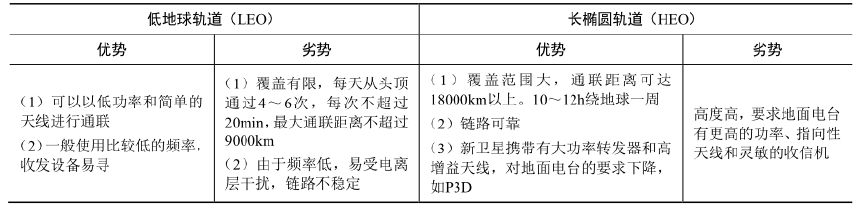
\includegraphics[width=0.7\linewidth]{87}
	\caption{}
	\label{fig:1}
\end{figure}

\begin{figure}[htbp]
	\centering
	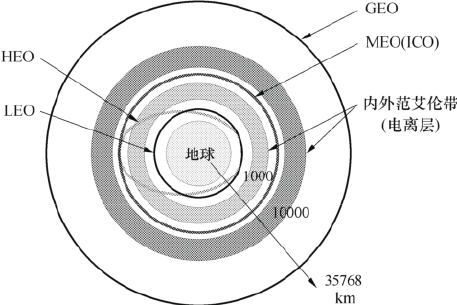
\includegraphics[width=0.7\linewidth]{88}
	\caption{卫星高度示意}
	\label{fig:1}
\end{figure}

(3)业余卫星通信操作需要的设备。根据目前正在运行的和即将发射的业余卫星情况,一个最基本的业余卫星地面电台由以下部件组成。
① 收信机:(能支持29MHz、145MHz、435MHz、2.4 GHz、10GHz和24GHz)。
② 发信机:(能支持21MHz、146MHz、435MHz、1.2 GHz、2.4 GHz和5.7GHz)。
③ 天线:要能支持你所需的全部频段。此外,由于卫星转发器都是设计成跨段收发的,所以要求天线收、发分离。同时也因为目前业余卫星多为沿轨道绕地旋转的,所以天线的仰角和方位角必须分别控制。天线系统对于地面业余电台来说十分关键,接收天线要能够提供良好的信噪比(噪声系数小于2dB),而发射天线则应能将足够的能量发送到卫星(增益大于12dB)。综合起来,天线需要着重考虑以下因素:
a.方向特性(增益值、增益方向);
b.发射和接收特性;
c.效率;
d.极化方向(收信天线圆极化);
e.连接效果(法拉第旋转和旋转调制)。

如果使用数据模式,还需要一个调制解调器(TNC)和计算机以及相应的软件。
4.卫星的转发器
卫星转发器有处理模拟信号和数字信号两类。目前模拟信号转发器为大多数爱好者所使用,模拟信号转发器又称线性转发器,它的作用是将上行频段内一组连续频率(频带)的信号经过放大,在另一个频段同样频宽的频带上重新发射。转发器将转发这个频带内的所有信号:SSB、CW、FM、数据、噪声、合法电台及非法电台等。业余卫星转发器的频带宽度一般为40~250kHz。
在描述卫星转发器的时候,通常将上行频率(或者波长)放在前面。比如“带有144MHz/29MHz转发器的卫星”就是表示这颗卫星的转发器能将144MHz上的某个频带转发到29MHz上。我们也可以将这个转发器称为2m/10m转发器或者叫A模式转发器。
5.业余卫星的模式
通信卫星的模式代表了该卫星转发器的上行频率(波长)、下行频率(波长)和发射方式。目前流行的命名法有两种。
(1)老式命名法,如表1-7所示。
表1-7 老式命名法

\begin{figure}[htbp]
	\centering
	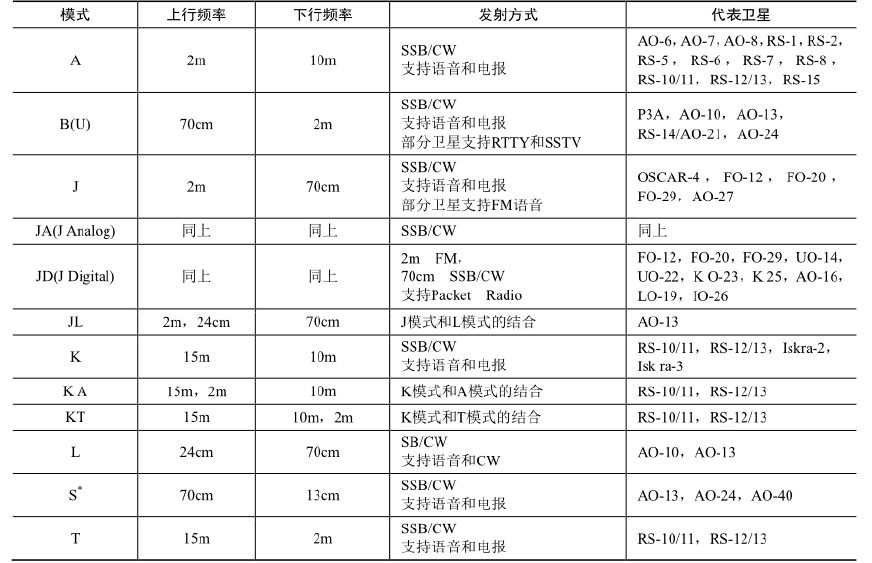
\includegraphics[width=0.7\linewidth]{89}
	\caption{}
	\label{fig:1}
\end{figure}

注:S模式原先设计为24cm上行/13cm下行,但这个约定从来没有被遵守。许多爱好者使用13cm~2m的变频器来将下行信号转换到一个2m的接收机上,而不必购买2.4GHz的接收机。
(2)新式命名法:频率代码。频率代码如表1-8所示。
表1-8 频率代码

\begin{figure}[htbp]
	\centering
	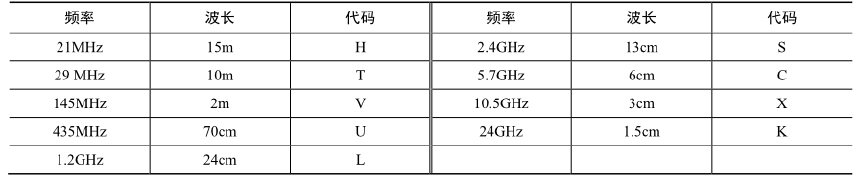
\includegraphics[width=0.7\linewidth]{90}
	\caption{}
	\label{fig:1}
\end{figure}

\begin{figure}[htbp]
	\centering
	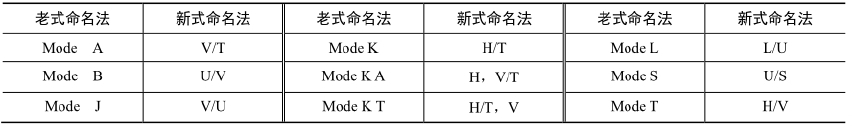
\includegraphics[width=0.7\linewidth]{91}
	\caption{表1-9 新旧命名法对照}
	\label{fig:1}
\end{figure}

6.业余卫星的分类
根据卫星运行轨道和功能,业余卫星可分为以下5类。
(1)1Phase 1,以OSCAR 1和2为代表的早期业余卫星,发射于20世纪60年代初期。这些卫星只携带低功率的信标台,寿命只有几个星期,如OSCAR 1~5。
(2)Phase 2,以OSCAR 6/ 7/ 8为代表的业余卫星,当前大部分可用的业余卫星均属此类。这类卫星最明显的特征是运行于低轨道(南北极地轨道或者低高度东西赤道轨道),因此爱好者只能在有限的时间内连接卫星,通联的范围也大大受到限制,如OSCAR 6~9,OSCAR 11~12,14~23,25~36,RS1~8,RS10~16等。

(3)Phase 3,Phase 3卫星的研究开始于20世纪70年代中期,这类卫星运行于长椭圆轨道之中。10~12小时绕地球一周,如OSCAR 10、13、40。之后一颗P3E是在2004~2005年间发射的。
(4)Phase 4,位于地球静止轨道上的业余卫星,目前此类的业余卫星都处在设计阶段。
(5)Phase 5,围绕月球或火星轨道运转的业余卫星,目前正在计划发射P5A。
7.卫星的跟踪
对于地面上的爱好者来说,业余卫星是移动的物体。因此,要想通过业余卫星进行联络,必须首先解决以下两个问题:我的电台何时能够“看”到某颗卫星?我的天线应该指向何处?
这两个问题曾经困扰了早期从事业余卫星通信的先驱们,随着计算机和信息技术的发展,人们开始利用计算机程序来找出答案。今天,计算机程序能够告诉我们更多的信息。
(1)卫星的操作约定,比如某颗卫星哪些转发器是开着的,使用哪一个信标(地面的控制人员有可能会切换卫星上的设置来改变卫星的操作方法)。
(2)计算频率的偏移,即多普勒效应。当波源与接收者之间相对运动时,接收者接收到波的频率会发生变化,这种现象被称为多普勒效应。明显的例子就是当你坐在汽车里听对面来车按喇叭时的感觉,声音由低到高再由高到低。由于业余卫星对于地球存在相对的运动,所以地面业余电台和卫星之间建立起来的连接也存在着频率漂移的现象。
(3)计算卫星天线朝向与地面电台天线朝向间的夹角以及卫星和地面电台间的距离。这些数据和通联信号的质量密切相关。
(4)当前卫星覆盖的区域,也就是当前能够通过卫星通联的地区。
(5)当前卫星是在阳光之中还是在地球的阴影之中。有一些卫星只能在位于阳光之中时操作。
(6)下一次和某地点能够通联的时间。由于卫星每次过顶的角度和高度不同,所以并不是每一次卫星过顶时都能够和某地点进行通联。许多爱好者还用辅助软件来控制天线的指向、补偿多普勒频漂或是解码卫星的遥感数据。有一些软件甚至还可以定时开关电台,并自动获取卫星上的数据。
常用卫星追踪软件如表1-10所示。
表1-10 常用卫星追踪软件

\begin{figure}[htbp]
	\centering
	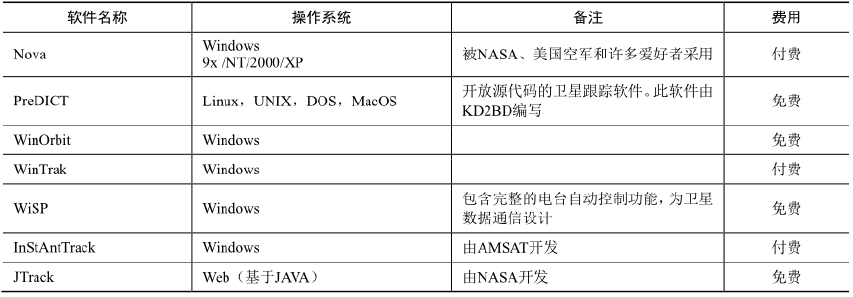
\includegraphics[width=0.7\linewidth]{92}
	\caption{常用卫星追踪软件}
	\label{fig:1}
\end{figure}

8.我国的“希望”系列业余通信卫星
我国恢复开放业余电台以来,涉足业余卫星通信的爱好者越来越多,国家对于普及卫星通信科学知识也给予了高度重视。
2009年12月15日10时31分,我国首颗搭载着业余无线电转发器的公益卫星“希望一号”(XW-1)在太原卫星发射基地升空并准确进入预定轨道。“希望一号”填补了我国业余无线电通信卫星项目上的空白,在国际业余无线电界引起了热烈反响,国际业余卫星组织将这颗卫星列入了国际业余卫星序列,编号为HO68。
2015年9月20号,我国又利用一箭多星技术,成功发射了“希望二号”系列业余通信卫星。希望二号系列卫星包括了XW-2A和2B、2C、2D、2E、2F共6颗卫星。
为能让更多的爱好者参与实验,国家无线电管理机构还于2010年1月做出决定,允许持有三级操作证书(2013年之后转换为A类操作证书)的业余无线电爱好者使用145.800~146.000MHz业余频段用于业余卫星通信实验。
XW-1采用整星框架加承力板结构设计,非等边的八边形立柱构形,星上能源采用体装太阳电池阵与锂离子蓄电池联合供电方式,卫星质量60kg,包络尺寸为680mm×480mm。这颗卫星运行轨道类型为太阳同步轨道,高度1200km,倾角105°,轨道周期为109min。所携带的遥测信标发射机发射频率为435.7900MHz,以CW方式工作;调频转发器下行频率435.6750MHz;线性转发器下行频率435.7650~435.7150MHz,SSB/CW模式;数据包存储转发器下行频率435.6750MHz,AFSK 1200bit/s模式。线性转发器上行频率145.9250~145.9750MHz,SSB/CW模式。其他方式上行频率均为145.8250MHz,其中数据包存储转发器标准为AFSK 1200bit/s,基于AX.25的PACSAT通信协议,星上的线性转发器和调频转发器不同时开启,开启方式由地面测控中心控制。
“希望一号”升空以后,我国爱好者通过星上转发器和国内外业余电台进行了频繁联络,许多爱好者用简单的天线装置就接收到了它的信标信号,在全国青少年业余无线电通信比赛中,小朋友们还练就了用手持简易天线和便携电台在户外快速跟踪和抄收卫星播发的遥测信号的本领。
希望二号A星(XW-2A)是一个边长为400mm的等边六面体,质量为25kg,能源为体装三结砷化镓太阳能电池阵和锂离子蓄电池联合供电。希望二号B、C、D星较小,均为边长250mm的等边六面体,质量9kg,能源和XW-2A一样。XW-2E和XW-2F则更为小巧,质量各为1.5kg。所有6颗卫星都配备有基本相同的业余无线电有效载荷,每颗卫星包括一个U/V模式线性转发器,一个CW遥测信标和一个数字遥测发射机。其中XW-2A运行在高度约450km的太阳同步轨道上,其他卫星运行在高度约530km的太阳同步轨道上。
希望二号系列卫星上行频率见表1-11,下行频率见表1-12。根据国际业余卫星组织网站截至2020年9月底的报告,各星业余通信载荷均工作正常。可以肯定,随着希望二号系列卫星的顺利发射,我国爱好者在业余无线电空间通信试验中一定会取得更加丰硕的成果。

表1-11 希望二号系列卫星上行频率
表1-12 希望二号系列卫星下行频率

\begin{figure}[htbp]
	\centering
	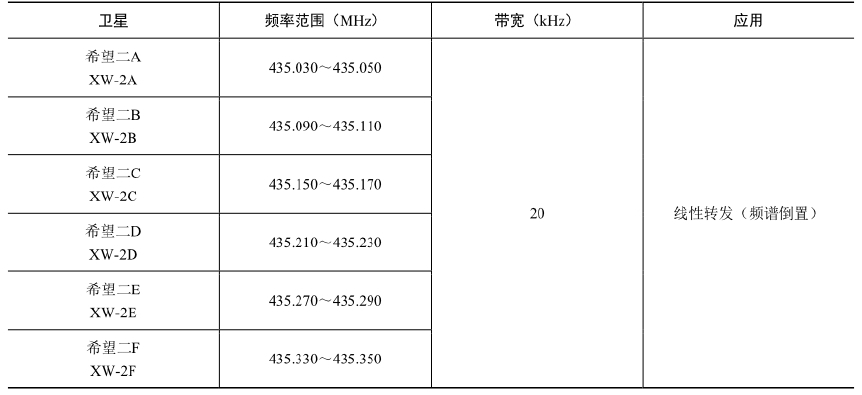
\includegraphics[width=0.7\linewidth]{93}
	\caption{}
	\label{fig:1}
\end{figure}

\begin{figure}[htbp]
	\centering
	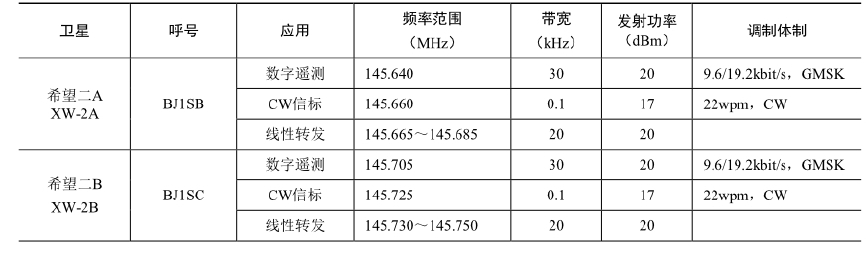
\includegraphics[width=0.7\linewidth]{94}
	\caption{}
	\label{fig:1}
\end{figure}

\begin{figure}[htbp]
	\centering
	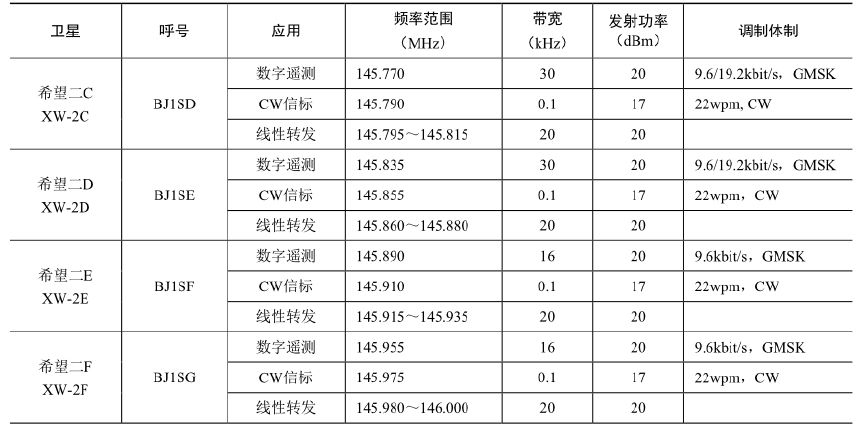
\includegraphics[width=0.7\linewidth]{95}
	\caption{}
	\label{fig:1}
\end{figure}

1.4.5 月面反射通信研究
月球是地球唯一的天然卫星,能不能利用月球把地面上发射出去的信号反射到地球上的另一个地点从而实现远距离通信呢?爱好者对此做出了巨大的努力,直至1960年由W6HB和W1BU两个美国业余无线电团体在1296MHz上首次实现利用月球表面无源反射进行的业余无线电双向通信。这种通信方式被称为“月面反射通信”(EME,Earth-Moon-Earth)。从此之后,探索者的队伍迅速壮大,世界各国的爱好者不懈努力,进行着各种模式的EME通信实验。在计算机技术尚不发达的时候,爱好者经常在50~1296MHz的各业余频段上用CW、SSB模式进行双向联络。美国ARRL等一些国家的业余无线电组织还组织EME通信的国际比赛。中国清华大学的业余电台BYIQH也曾在1997年10月19日,用2m波段成功地和瑞典SM5FRH等业余电台进行了我国第一次双向EME试验。
随着计算机技术的发展和普及,具有自动纠错功能的数据交换方法和程序不断涌现并被用于无线电通信,业余无线电爱好者也编写出了如著名的JT65那样的适用于极弱信号环境下的无线电通信协议(见本章1.4.2之5),实现可靠EME 通信的愿望已非遥不可及。
1.4.6 移动通信研究
与穿梭在城乡天地间安装在各种交通工具上的业余电台、临时架设进行业余无线电通信实验和竞赛的电台、参与配合突发事件应急通信的业余电台间的通信都属于业余无线电移动通信。如何在没有商业移动通信网络(如手机、卫星电话)条件下,利用广泛生存于民间的设备搭建起畅通的业余无线电移动通信网,是世界各国爱好者又一个不懈努力的方向,而要获得可靠、快速、多模式的通信效果,依然面临着许多待解之题。
许多国家定期举行大范围的移动通信活动日。如美国每年6月最后一周的星期六和星期日为“户外日”(Field day),每到这一天,爱好者就把自己的电台设备带到野外相互联络,唯一的要求就是不用市电。我国爱好者也经常组织各种活动,如“业余无线电应急通信演练”“无盲区天线通信比赛”“V/U通信日”等,试验和改进天线装备,检验和熟练运用各种通信手段的能力技巧,锻炼和提高了业余无线电爱好者在突发性自然灾害中服务于社会应急通信并为之做出贡献的能力。
1.4.7 小功率通信研究
世界上许多爱好者热衷于用只有几瓦甚至更小功率的电台进行远程通信试验,他们为如何利用尽可能小的发射功率,联络到距离尽可能远、范围尽可能广的业余电台而发着“高烧”,并因此而不断地推出一些性能优良的小功率电台,而利用不到5W功率的QRP小功率业余电台,沟通全球并取得WAC奖状的爱好者,在世界上已不乏其人。在对保护电磁环境的要求越来越高的今天,用尽可能小的发射功率实现更远距离的通信有着非常重要的现实意义,而层出不穷的面向微弱信号无线电数字通信软件也使得QRP小功率通信有了更加广阔的天地。
1.4.8 V/U波段通信
V/U波段通信泛指30~3000MHz的通信,其中30~300MHz为VHF段(甚高频),300~3000MHz为UHF段(特高频)。
在许多国家制定的业余无线电操作等级标准中,都规定了初级操作员只能使用V/U波段进行发射活动。我国也是如此,V/U波段成为所有爱好者加盟业余无线电之后的首用频率。
在我国,VHF段中的业余频段有50~54MHz、144~146MHz、146~148MHz。其中144~146MHz为业余业务专用频段,其余两段均为和其他业务共用的频段,且50~54MHz业余通信是次要业务。UHF段中属于业余频段的有430~440MHz、1240~1300MHz、2350~2450MHz,这3段均为和其他业务共用的频段,而且业余业务都是次要业务。
V/U波段包括了大量专业业务的通信,如航空导航、卫星通信、广播电视及交通、公安、消防等固定或移动业务,这些通信关系着人民的生命财产,关系着社会的安全稳定,十分重要。每一个业余无线电爱好者,都必须严格遵守国家有关法令,不在这些非业余无线电频率上进行发射和收听。对于业余业务属于次要业务的频段,各地无线电管理机构根据当地的情况,有可能对业余无线电通信采取部分禁用或限用的措施,我们应该了解和严格遵守。
V/U波段电磁波的传播方式主要是直线传播,“视距通信”是这个波段通信的特点。在这个波段里,一般情况下通信距离取决于电台所在位置,双方天线之间没有高大建筑物或山地阻挡,小功率也可以实现远距离通信。
在V/U波段中,144MHz(2m)频段和430MHz(70cm)频段是爱好者的“入门波段”,也是业余无线电“人气”最旺的地方,世界上数以百万计的爱好者中,70\%活跃在这个波段上。爱好者们可以通过手持式对讲机或车载电台,在数千米范围内进行实时联络,也可以通过由业余无线电组织设置的中继台在数十千米范围内相互交流通信,十分方便。
如何选择V/U波段通信设备?常见的设备均为FM调频模式,除了工作频率及发射功率必须是在无线电管理机构批准的和你的业余通信操作允许范围内,其实用性是最主要的。通过销售商用电脑设置频率(即写频)的设备也可以使用,但不很方便。收、发频率最好可以分别设置,这对于能否使用当地的中继系统是很重要的。电池块、充电器等配件、附件应较易获得。有关业余无线电设备的介绍见本书第7章。
我国每年的5月、6月、7月,是144MHz传播条件最好的时候,“中、日、俄、韩2m通信试验”已经吸引了内地及香港、澳门特别行政区及我国台湾地区的许多爱好者,通信距离的纪录不断被刷新。144MHz也是EME“月面反射通信”的常用频段。这些通信实验一般使用SSB单边带模式,爱好者通常选用集HF短波和VHF超短波于一体、功率较大的设备进行。
50MHz(6m)频段是高频与甚高频之间的临界频段,其传播特性也最为奇特。冬季的早晨,周边国家的信号如同本地台那样清晰响亮,捕捉“突发性E层”和捉摸不定的流星余迹进行超远程通信是这个频段最具魅力的课题之一。不过,我国南京等城市因为广播电视仍在使用这个频段,6m波段业余通信还只能停留在“收听”阶段。
对于1200MHz以上频段,我国爱好者也已涉足,并取得一定的成绩。在这些频率段,利用其比较宽的频带,进行速度更快、保密性更强的无线电数据通信,如“扩频通信”已经成为现实。1200MHz以上频段,由于波长极短,天线、元器件出现了新的形态,延长相互间的通信距离变得更为困难,向更高的频率进军,为人类开发新的电磁波资源,正是这些频段对无线电爱好者提出的挑战。

1.4.9 网络业余无线电
1.VoIP网络业余无线电通信
在国际互联网和计算机技术飞速发展的浪潮中,一种将业余无线电和网络技术结合起来的新的通信方式应运而生。人们把这种通信方式称之为VoIP。VoIP(Voice-Over-IP)即语音信号通过互联网在不同的IP地址之间传递。司空见惯的“网络通话”过程是,语音信号经计算机声卡转变为数字信号,通过相应软件的控制,经过互联网的传递,再由另一台计算机将此数据流接收下来并经过相应软件处理,还原成语音输出。而VoIP与这种通常的网络通话所不同的是,语音信号的来源和输出对象都是业余电台。一部移动使用的手持式对讲机或是一部车载电台通过中继装置(被称为“节点”)与互联网中特定的服务器相连,自己的声音被传送到网络另一端,再通过接收端中继台和另外一个移动或者固定的业余电台进行QSO。当然,也可以直接利用计算机通过网络呼叫这个VoIP系统中的其他电台,完成“交叉”方式EQSO。
世界各国的爱好者在这一通信试验中,建立了不同的数据标准,编写了不同的软件,通过不同的硬件和网络系统中的服务器,建立了不同的VoIP系统。爱好者们可以通过计算机找到这些网站,下载相应的软件,在电台和计算机之间建立起必要的连接,并按照要求加入这些系统中去。目前常见的VoIP系统有以下几种。
(1)IRLP。它的设计者是加拿大爱好者David Cameron,VE7LTD。IRLP系统自1997年11月问世以来,经过不断的完善和改进,有了比较成熟的软硬件支持,获得了众多爱好者的青睐。
(2)EchoLink。这是我国爱好者比较熟悉的一个VoIP系统。各地的业余无线电网,如本地的中继台,通过“地方主控台”也即“节点”,汇合到网络中的会议服务器上。一些分散在偏远地方的HAM也可以直接进入会议室。通过系统软件,我们可以看到遍布世界各地登录在EchoLink系统中的全部成员的动态信息,并有可能听到其中任一电台的声音并与之QSO。EchoLink网站可以指导你如何成为这个系统的一员。
(3)WIRES-Ⅱ。这个系统最初是由美国爱好者创立的,经过不断的改进和完善,现在成为了日本YAESU公司商品生产的一部分,由该公司为业余无线电设备提供完整的网络连接硬件和软件包。据称日本近80\%的HAM、世界各国有近两千个业余电台加入这个系统。
(4)D-star。这个VoIP系统是由日本业余无线电联盟JARL创造的,现在已经嵌入日本Icom公司生产的收发信设备当中。
VoIP通信把分散在世界各地的业余电台通过互联网紧紧联系到了一起,DX变得不再遥远,QSO更加便捷可靠。由于在应急通信中可能发挥的独特作用,这种通信方式正在得到业余无线电组织和社会各界越来越多的关注和重视。
当然,由于技术和网络安全的原因,目前还没有办法把各种VoIP统一为一体,让人们体验到与真正的DX联络一样的宽广和自由,但可以相信,爱好者的这个梦想一定会变为现实。

2.WebSDR网络软件无线电
软件无线电(SDR,Software-Defined Radio)是20世纪90年代兴起的一项新技术,其基本思想是将硬件作为通用的基本平台,把尽可能多的无线电通信功能通过可编程软件来实现,使无线电系统可以灵活地实现各种功能,并可以在硬件平台基本结构不变的情况下,通过改变软件来改进升级、使用新技术。SDR已经成为现代无线电技术的重要发展方向。
WebSDR(Web-Software-Defined Radio),我们把它称之为网络软件无线电。这是软件无线电技术和互联网技术相结合的产物。爱好者们运用计算机技术设计制造出高质量的宽频带收信机,并在电磁环境良好的地方建立收信台。他们把收信机收到的信息实时上传到互联网上,只要登录这些网站,你的计算机就成了一台软件无线电收信终端,可以收到从异国他乡收信台上传的各种无线电信号,不必架设电台便可领略业余波段上热闹非凡的奇妙景象。
要体验WebSDR并不困难,先下载免费的JAVA系统,然后浏览WebSDR链接中的收信台网址。这时,业余波段的频谱图便显示在网页下方。你可以任意选择其中的波段、频点,变换工作模式和频带宽度,非常清楚地收听到欧美“本地电台”在和远方的DX电台通联。如果你已经有了短波电台,还可以通过WebSDR检测一下自己的信号传到远方是否够强。
3.OpenWebRX开源网络软件无线电
OpenWebRX 是无线电爱好者HA7ILM(AndrásRetzler)创建的开源项目,也是基于Web的频谱接收解调工具,该工具已在全球200多个服务器中使用。不同于WebSDR,OpenWebRX更加开放,更加注重在小型轻量化硬件设备上实现各种模式尤其是数字通信模式的解调,比如与OpenWebRX同时推出的KiwiSDR硬件项目,在安装完成OpenWebRX系统后只需要插上电源和网线,即是一台可以随时访问的、同时显示0~30MHz带宽的在线SDR设备,支持多用户同时访问,并且不需要第三方软件就可在网页上完成如CW、DRM、SSTV等模式的解调工作。另外在PC机或“树莓派”上结合RTL-SDR设备也同样可以实现以上功能,甚至还可实现在线解调如FT8、DMR、PACKET等功能。
OpenWebRX原项目创始人已停止开发,但作为开源项目产生了多个分支团队继续进行更多功能的开发工作,如果感兴趣可登录相关网站获得更多信息。
4.SDR-RADIO V3网络软件无线电
SDR-RADIO V3网络软件无线电是Windows平台上功能强大的SDR接收软件,其中提供了将本机所使用的SDR设备转变成可在线远程操作的服务端应用。与上述网络SDR软件不同的是,SDR-RADIO V3自身支持的SDR硬件相当丰富,另外即使远程连接在线SDR服务器,其操作同控制本地设备那样完全相同的。由于可以轻松搭建服务器,远程用户体验感更好,扩展性更强,受到广大无线电爱好者喜爱,全球也分布着众多的服务器。
5.SDR\#网络软件无线电

与SDR-RADIO V3类似,SDR\#也是一款广受欢迎的SDR软件,其中也集成了远程SDR的连接客户端功能。不同的是硬件主要集中在自己开发的AIRSPY系列硬件和市场较多的RTL-SDR设备。
6.电台远程控制系统RCForb
RCForb是一个无线电团体合作开发的一款电台远程遥控软件,可以安装在手机或者PC电脑上。这样,无论身在何处,只要拿出手机或者PC电脑,就可对家中或俱乐部电台的天线和短波电台设备包括转向器、功放及天线切换器进行遥控操作,享受操作远程电台的乐趣。
RCForb软件可在remotehams网站注册并下载。
1.4.10 业余无线电测向
业余无线电测向,英文名Amateur Radio Direction Finding(ARDF),又被称为“猎狐”(Fox Hunting),是由欧洲的爱好者于20世纪40年代发起的集业余无线电技术和户外运动于一体的一项活动。爱好者们借助自己制作的具有准确方向性的天线和接收机,运用电波传播知识和业余无线电操作技能,准确探测出发射机方位并迅速找到这些电台是这项活动的基本形式。国际业余无线电联盟(IARU)为业余无线电测向活动规定了使用频率(3.5MHz和144MHz业余波段范围内)和测向电台的专门呼号(MOE、MOI、MOS、MOH、MO5以及终点信标MO等),并制定了业余无线电测向世界锦标赛竞赛规则。
由于这项活动所特有的趣味性和挑战性,几十年来吸引了世界各国大量业余无线电爱好者和青少年参加,国际业余无线电联盟和许多国家的业余无线电组织也把这项活动作为帮助更多的人了解和体验业余无线电乐趣的户外运动项目来加以普及和推广。
本书附录23介绍了业余无线电测向机的设计与制作方法,旨在帮助有兴趣的朋友更多地了解这方面的知识。

\subsection{数字通信}

数字通信是指传递数字信号的通信模式。通信的数字化,是当今通信技术的发展趋势之一。业余通信中的数字通信模式可以说是层出不穷,直到今天还在业余界广泛使用的电报(CW)应该算是最古老的一种数字通信模式。无线电电传(RTTY)是一种对设备要求较低的数字通信模式,在发送端用键盘代替话筒或电键输入信息,接收端则把来自对方的文字显示在显示器上,如图1-3所示。AMTOR是一种具有纠错码功能的电传通信方式。这种通信方式把每一个信息分散在不同时间里重复发送,在不增加设备的情况下,可以大大改善通信系统的可靠性。

\begin{figure}[htbp]
	\centering
	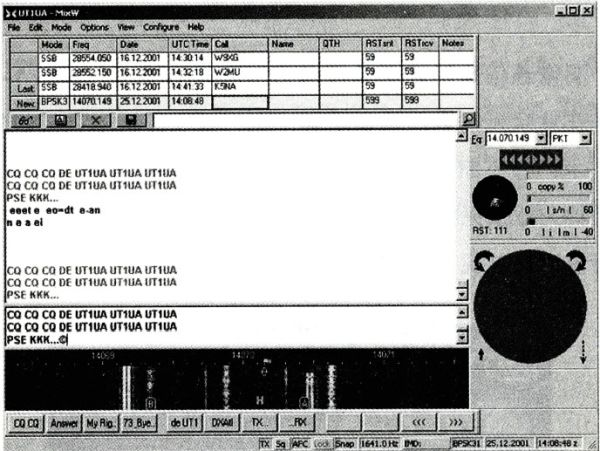
\includegraphics[width=0.7\linewidth]{3}
	\caption{数字通信软件}
	\label{fig:1}
\end{figure}

PSK31是指带宽为31Hz的移相键控调制模式。它只需要31Hz的带宽,占用频带非常窄,抗噪声能力强。当非常微弱甚至是几乎不可闻的信号出现时,只要在计算机屏幕上能出现信号轨迹,一般都能正确地解调。

另一种被广泛使用的数字通信模式是PACKET,利用广泛存在的PACKET网络,业余爱好者们每时每刻都能传递各种各样的信息,美国的爱好者甚至还利用PACKET网络提供全国范围的业余定位系统服务。

除此之外还有PACTOR、CLOVER、G-TOR等其他的数字通信模式,每种不同的模式适合不同的应用场合,各有各的特点。各种模式的通信实验给热衷于数字通信的业余无线电爱好者带来了许多乐趣。

\subsection{图像通信}

图像通信是现代通信技术综合发展的结果,如图1-4所示。在业余无线电通信领域里,也一直在探讨电视图像的传送技术,并不断对其进行改进。图像通信有两种主要方式;一种称为业余无线电视(ATV),用于传送活动图像;另一种称为慢扫描电视(SSTV),用于传送静止图像。

\begin{figure}[htbp]
	\centering
	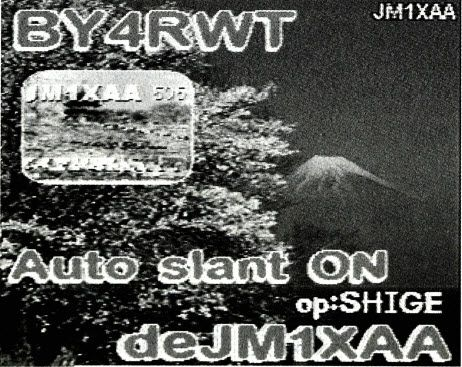
\includegraphics[width=0.7\linewidth]{4}
	\caption{图像通信}
	\label{fig:1}
\end{figure}

普通电视为保证图像清晰,每秒需传送50幅图像,要占用6MHz宽的频带。业余频段范围较窄,难以传送一般的电视信号。爱好者采用几秒传送一幅图像的办法,用图像信号的慢变化来减小频带宽度,使得在短波波段传送图像的愿望得以实现。现在,许多爱好者借助计算机技术,配合简单的接口电路及软件,就可以完成SSTV方式的通联,这极大地丰富了业余无线电通信的内容。

\subsection{业余卫星通信}

1957年10月4日前苏联发射了世界上第一颗人造地球卫星,与此同时,美国的一些爱好者萌发了发射业余通信卫星的设想。他们组织起来并将这个计划命名为OSCAR。4年之后,他们的努力获得成功,世界上第一颗业余通信卫星OSCAR-1号在美国加利福尼亚的范登伯格空军基地发射升空。这不但证明了业余无线电爱好者有能力研制、开发、控制自己的卫星,也标志着业余无线电通信从此进入了太空时代。

业余卫星通信系统分为空间部分和地面部分。空间部分是指业余通信卫星,地面部分就是我们的业余电台。一个业余卫星地面电台由收发信设备、天线和跟踪控制系统组成。

在卫星通信中,由于通信距离远,信号传输损耗较大,卫星通信天线需要有较高的增益。VHF/UHF频段多采用8~10单元的八木天线,更高的频段使用20单元的八木天线或是抛物面天线。由于低轨道卫星运行周期较短,天线系统还应具备自动跟踪的功能。一般把发送、接收天线集中安装在可沿水平轴和垂直轴旋转的云台上,根据室内提供的驱动信号完成跟踪。

业余卫星通信爱好者可以选用专用的卫星收、发信机,能够异频双工工作。如YAESU公司的FT-736就是一种VHF/UHF频段全模式的卫星收、发信机,能在50MHz、144MHz、220MHz、430MHz和1200MHz业余波段工作,有SSB、CW和FM模式,能够同时异频收、发。这对于在低轨道卫星通信中克服多普勒频移很有作用。

低轨道卫星的特点是运行速度快,一般每两小时绕地球一周。要与低轨道卫星通信,必须能精确地确定卫星的位置。现在已有专门的软件可以计算出业余卫星的轨道,可以知道卫星什么时候经过我们的上空,算出卫星的仰角和方位角,由计算机控制天线方向控制器,使天线始终指向卫星,自动完成对卫星的跟踪,如图1-5所示。由于天线的波束宽度有一定的范围,也可通过手动方式控制天线方向。

\begin{figure}[htbp]
	\centering
	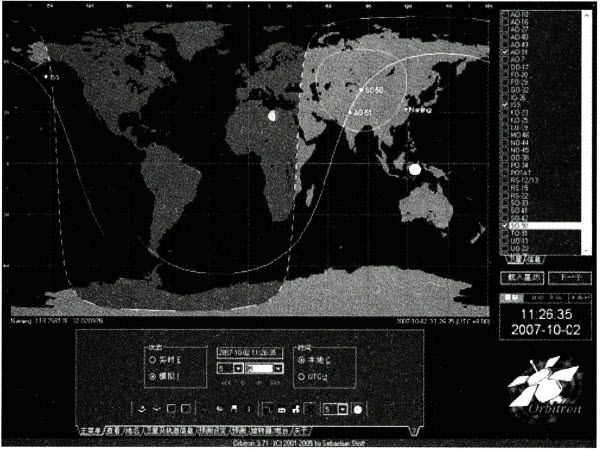
\includegraphics[width=0.7\linewidth]{5}
	\caption{卫星跟踪软件}
	\label{fig:1}
\end{figure}

世界各国的业余无线电爱好者已经成功地发射了二十几颗业余卫星。2009年12月15日,“希望一号”卫星(HO-68,见图1-6)在太原卫星发射中心搭载“长征四号丙”运载火箭成功地进入太空,见图1-7。这是中国第一颗青少年科普卫星。广大的业余无线电爱好者可以通过“希望一号”卫星进行各种方式的通信实验。

\begin{figure}[htbp]
	\centering
	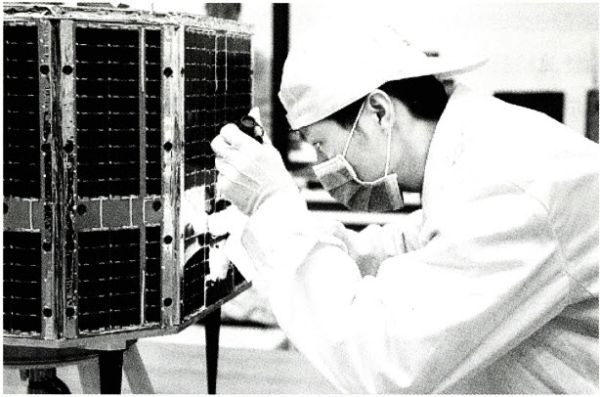
\includegraphics[width=0.7\linewidth]{6}
	\caption{技术人员在测试“希望一号”卫星}
	\label{fig:1}
\end{figure}

\begin{figure}[htbp]
	\centering
	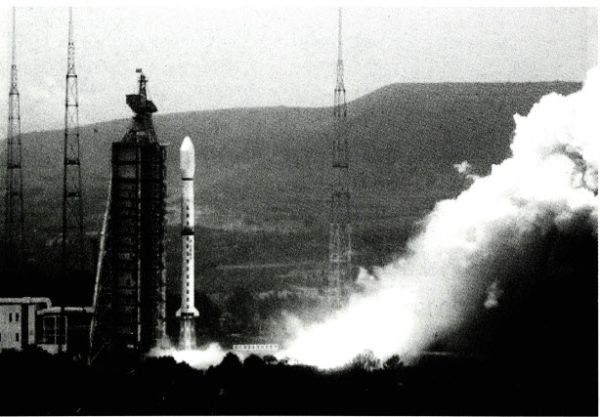
\includegraphics[width=0.7\linewidth]{7}
	\caption{“希望一号”卫星搭载“长征四号丙”运载火箭成功进入太空}
	\label{fig:1}
\end{figure}

\subsection{国际空间站业余无线电通信计划}

和国际空间站宇航员对话是一种独特的体验。国际空间站业余无线电通信计划(ARISS)是由美国业余无线电协会、国际业余卫星公司、美国国家宇航局等共同组织和发起的一项活动,是美国国家宇航局面向青少年的科技教育项目之一,图1-8所示为美国等16个国家共同建造的国际空间站。这个计划给学生们提供了一个利用业余无线电和国际空间站宇航员直接交流的机会。该计划要求学生用英语提出有关太空、太空飞行、宇航员的太空生活等的问题,宇航员对学生提出的问题进行解答。因此要求学生有较好的英语口语和听力水平,同时对太空知识有一定的了解。从2000年到2010年,世界上大约有400所学校参与了这项活动。

\begin{figure}[htbp]
	\centering
	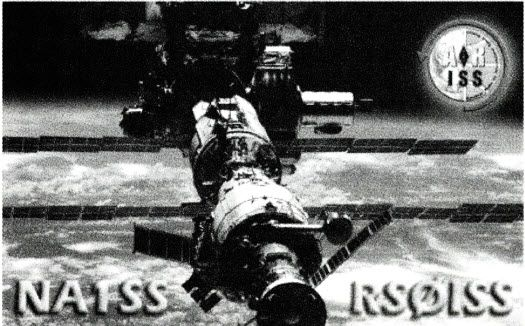
\includegraphics[width=0.7\linewidth]{8}
	\caption{国际空间站}
	\label{fig:1}
\end{figure}

“Can you see the Great Wall from the ISS?”2007年8月26日北京时间18:44,南京市第三中学初二学生唐洁雯用流利的英语向宇航员提出了第一个问题,克莱顿·安德森在距地球300km的国际空间站上听到来自中国学生的呼叫。经过两年的不懈努力和等待之后,BY4RRR与国际空间站的通联活动终于得以实现。图1-9所示是中国学生第一次通过ARISS的国际计划,直接与国际空间站上的宇航员对话的情景。

\begin{figure}[htbp]
	\centering
	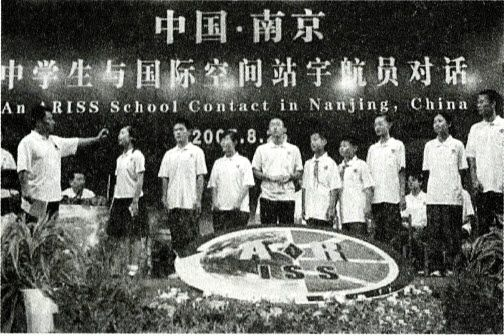
\includegraphics[width=0.7\linewidth]{9}
	\caption{BY4RRR的同学与国际空间站宇航员对话}
	\label{fig:1}
\end{figure}

\subsection{月面反射通信}

依靠月面反射完成通联的这种通信方式称为EME(Earth Moon Earth),见图1-10。地球与月球之间的距离大约为380000km,电波往返一次衰减极大,月面反射通信返回到地面的信号非常微弱。要想完成一次EME联络,必须掌握无线电波的传播特点,知道月亮的阴晴圆缺产生的不同的天体噪声对接收的影响。进行EME通信必须配备大功率发射机、高增益天线(见图1-11)以及高灵敏度的接收机。目前,完成双向EME联络大多数为CW方式。

\begin{figure}[htbp]
	\centering
	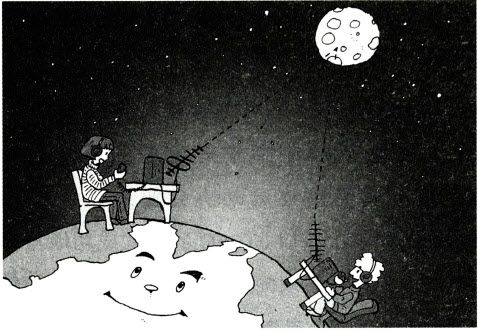
\includegraphics[width=0.7\linewidth]{10}
	\caption{月面反射通信}
	\label{fig:1}
\end{figure}

\begin{figure}[htbp]
	\centering
	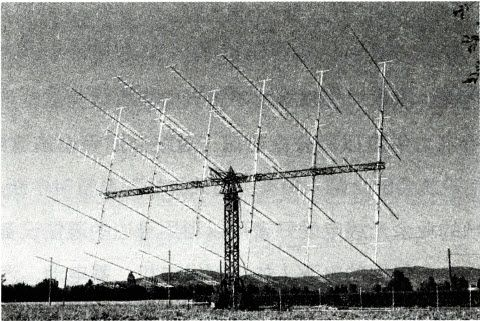
\includegraphics[width=0.7\linewidth]{11}
	\caption{用于月面反射通信试验的八木天线阵}
	\label{fig:1}
\end{figure}

20世纪40年代,业余无线电家们已向EME通信发起了挑战。经过许多次失败之后,终于在1960年,美国的W6HB和W1BU在1296MHz首次实现了EME通信。

我国业余无线电爱好者也在积极探索EME通信。1997年10月19日,清华大学业余电台BY1QH在2m波段和瑞典SM5FRH等业余电台成功地进行了双向的EME联络,实现了我国在这一领域零的突破。

现在,EME通信已采用由计算机完成的新的调制技术,这大大降低了EME通信对设备的要求。2007年5月20日,江苏省无线电运动协会业余电台BY4RSA在1296.090MHz频率上,以JT65C的模式成功地与荷兰的业余电台PA3CSG进行了双向EME通联。这次实验使用的是一台IC706电台,一个自制的变频器和直径为1.8m、增益为25dB的抛物面天线,一台自制的功率放大器,发射功率仅90W。

\subsection{应急通信}

当地震、洪水、恐怖袭击等重大灾害事故突然发生时,往往伴随着电力供应以及公众电信、道路交通等设施遭到破坏,常规通信设施会随之陷入瘫痪,与外界的联系暂时中断。这时,灾害现场的业余无线电爱好者可以利用身边的通信设备,尽快找到可供电台使用的电源(如小型发电机、蓄电池、汽车电源等),选择有利地形,迅速架设天线,并立即进行紧急“求救呼叫”。在美国“9·11”恐怖袭击事件、印尼大海啸、四川汶川地震等灾难中,业余无线电爱好者在应急通信中都发挥了重要的作用。

在VHF/UHF频段,可用语言直接进行求救呼叫。

例如:“May Day、May Day、May Day! BA4AAA求救,BA4AAA求救,听到请回答。”

在求救呼叫得到灾害现场以外地区的回答后,呼救电台应向外发送以下信息:

①受灾的精确地点及性质(即遭受何种灾害);

②受灾的程度及受灾现场的情况;

③灾害现场现有的救援力量及迫切需要何种支援。

④其他一切有利于援助的资料。

求救呼叫是最高级别的信号,任何业余电台收听到求救呼叫时,必须立即无条件中断发射,改为守听状态,并给予必要的协助。

呼救电台在紧急情况得到解决后,应及时在结束联络时清楚地发出解除呼救的信号,以免其他电台继续长时间守听。
例如:“我是BA4AAA,救援人员已经到达,BA4AAA解除呼救,BA4AAA解除呼救,再见。”

承担救灾应急通信是业余电台的社会责任和优良传统,也是业余频段得到保护的主要理由之一。世界上许多国家都成立了业余无线电应急服务组织,美国ARRL有专业的业余无线电通信应急服务(ARES)委员会,我国的无线电爱好者也在积极开展应急通信演练活动(见图1-12),筹划、建立各地区的业余无线电应急通信网络。

\begin{figure}[htbp]
	\centering
	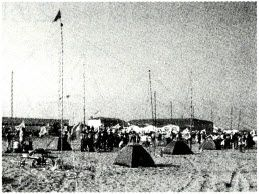
\includegraphics[width=0.7\linewidth]{12}
	\caption{应急通信演练}
	\label{fig:1}
\end{figure}

\section{业余电台的分区}

为便于管理,国际上和每个国家都根据地理位置,将世界和本国国土划分为若干分区(ZONE),最常用的国际性分区主要有国际电信联盟的“ITU分区”和美国CQ杂志的“CQ分区”两种。

ITU分区将世界分为75区,中国属于其中的第33、42、43、44、45(钓鱼岛)、50(黄岩岛)区。CQ分区将世界分为40区,中国属23、24、25(钓鱼岛)、27(黄岩岛)区。

国内分区是指有些国家或地区把本国本地区范围内的业余电台按其地理位置划分的区域,我国境内除港澳台地区外的业余电台分区共分为0~9,10个分区。

第1区——北京、卫星业余业务 第6区——安徽、河南、湖北

第2区——黑龙江、辽宁、吉林 第7区——湖南、广东、广西、海南

第3区——天津、河北、内蒙古、山西 第8区——四川、重庆、贵州、云南

第4区——上海、山东、江苏 第9区——陕西、甘肃、宁夏、青海

第5区——浙江、江西、福建 第0区——新疆、西藏

香港为VR2,澳门为XX9,台湾地区为BV。


\section{依法设置业余电台}

为了有效利用无线电频率资源,保证各种无线电业务的正常进行,国际电信联盟制定了无线电管理的国际法规——《无线电规则》,用来作为各国无线电管理的依据。1993年国务院、中央军委颁布了《中华人民共和国无线电管理条例》,国家无线电管理机构先后颁布了一系列规章和管理文件。这些规定是我们开展业余无线电活动必须遵循的准则。
业余无线电爱好者不同于一般的电子技术爱好者,设置和使用个人业余电台,进行无线电波的发射,必须向国家或者地方无线电管理机构提出申请,得到批准并取得《中华人民共和国无线电台执照》(以下简称《电台执照》),严格按照指配的频率、功率工作。未经批准擅自使用无线电通信设备,干扰其他无线电通信业务的正常工作,造成空中电波秩序混乱,违规者将受到警告、查封及没收设备、罚款、吊销《电台执照》等处罚。造成严重后果、构成犯罪的,将依法追究刑事责任。

\subsection{取得业余电台《操作证书》}

根据国家无线电管理机构的有关规定,设置个人业余电台必须持有《中华人民共和国业余无线电台操作证书》(以下简称《操作证书》),如图1-13所示。《操作证书》是设置操作业余电台所要求的技术凭证。它共分5个等级,一级为最高级,五级为收听级。

\begin{figure}[htbp]
	\centering
	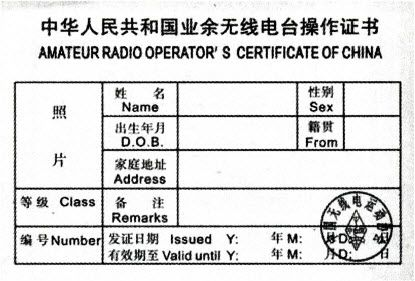
\includegraphics[width=0.7\linewidth]{13}
	\caption{《中华人民共和国业余无线电台操作证书》}
	\label{fig:1}
\end{figure}

申请《操作证书》者,应是经过无线电管理机构委托的中国无线电运动协会或其他单位的培训,并经《操作证书》考核机构考试合格的中华人民共和国公民。申领《操作证书》没有年龄限制。

取得《操作证书》后,可凭证在国内的个人和集体业余电台上进行操作,但必须得到电台的设台人或负责人同意,使用所操作电台的呼号,并严格遵守该台及《电台执照》中的各项规定。操作时使用的功率、频率及操作方式不得超越本人《操作证书》允许的范围。

取得《操作证书》后,如果打算设置个人业余电台,可按当地无线电管理机构规定的渠道递交《设置个人业余电台申请表》,并按当地无线电管理机构的要求对电台设备进行检验、检测,批准并核发《电台执照》,如图1-14所示,同时指配业余电台呼号。只有获得《电台执照》后,爱好者才能使用分配给自己的呼号,按照规定与国内外业余电台进行联络和交换QSL卡片。

\begin{figure}[htbp]
	\centering
	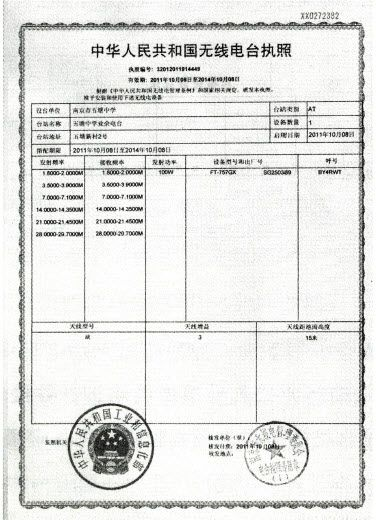
\includegraphics[width=0.7\linewidth]{14}
	\caption{《中华人民共和国无线电台执照》}
	\label{fig:1}
\end{figure}

\subsection{设置业余电台}

需要注意的是,部分初学者不了解有关的法规,购买到对讲机等通信设备后,自行设置频率,无证(照)发射。或虽有《操作证书》和《电台执照》,但使用时随意改变《操作证书》所允许的频率、功率范围,干扰其他电台,这都是与有关法规相违背的。

\subsection{工业和信息化部无线电管理局}

工业和信息化部无线电管理局是国家无线电管理机构,负责无线电频率的划分、分配与指配;依法监督管理无线电台(站);负责卫星轨道位置协调和管理;协调处理军地间无线电管理相关事宜;依法组织实施无线电管制;负责无线电监测、检测、干扰查处,协调处理电磁干扰事宜,维护空中电波的秩序。国家无线电管理机构和地方无线电管理机构负责业余电台的管理工作。

4.中国无线电运动协会
中国无线电运动协会(CRSA,见图1-15)是全国无线电爱好者的群众性组织,是主管业余无线电活动的政府部门联系广大无线电爱好者的纽带和管理业余无线电活动的助手。中国无线电运动协会在国际业余无线电联盟(IARU)中代表中国业余无线电爱好者。

\begin{figure}[htbp]
	\centering
	
\includegraphics[width=0.7\linewidth]{15}
	\caption{CRSA会徽}
	\label{fig:1}
\end{figure}

目前,不同省、自治区、直辖市的业余无线电爱好者加入中国无线电运动协会,参加业余电台操作培训和考核,申请设置使用业余电台所需履行的具体手续有所不同,可向当地无线电管理机构、中国无线电运动协会或地方业余无线电社团咨询。中国无线电运动协会的总部设在北京,通信地址为“北京6106信箱”,邮政编码:100061,网址www.crsa.org.cn。

\subsection{国际电信联盟}

国际电信联盟是联合国的一个专门机构,也是联合国机构中历史最长的一个国际组织,简称“国际电联”、“电联”或“ITU”。国际电联是主管信息通信技术事务的联合国机构,主要负责各种业务间的频率分配。国际电联总部设在瑞士日内瓦,其成员包括191个成员国和700多个部门成员。

\chapter{选购一部业余电台}

引子
最好的选择未必是选择最好的。

可供爱好者选择的业余电台品种很多。按照不同的分类方法,可将业余电台分为单波段电台、双波段电台、多波段电台,或是手持式电台、车载电台、短波电台和全波段电台。尽管各种电台的外形、大小不尽相同,每部电台都由一些基本组件构成,它们是:电源、发射/接收机和天线,如图2-1所示。

\begin{figure}[htbp]
	\centering
	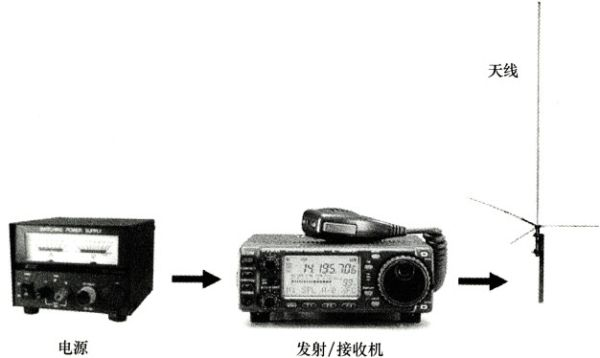
\includegraphics[width=0.7\linewidth]{16}
	\caption{电源、发射/接收机和天线是业余电台的3个基本组件}
	\label{fig:1}
\end{figure}

业余电台是指可以工作在业余频段的电台设备。购买电台之前,先要知道与电台设备密切相关的一些知识,如频率、频段、调频、调幅、功率等,以便在选购时对电台的特点有一个初步的了解。购买电台需要考虑许多因素,首先要确定电台的类型,然后再根据通信距离和通信环境来选择工作频段及输出功率。电台又是一种特殊的商品,购买、使用时还必须了解有关的法规和政策。

\section{业余频段}

人们可利用的电磁波的频率从千分之几赫直至1030Hz。为了便于研究、使用和管理,国际上把整个无线电频谱划分为若干频带,通常称为频段或波段。无线电波频段的划分见表2-1。电磁波是人类共享的资源,为了合理使用这一资源,国际电信联盟(ITU)对广播、移动等各种无线电业务可以使用的频率作了规定和划分。业余无线电通信作为业余业务在各频段上也都占有一席之地。这就是供全世界业余无线电爱好者使用的业余频段,我国业余电台使用的频率以《中华人民共和国无线电频率划分规定》为依据,表2-2列出的是常用的业余频段名称和频率范围。

\begin{figure}[htbp]
	\centering
	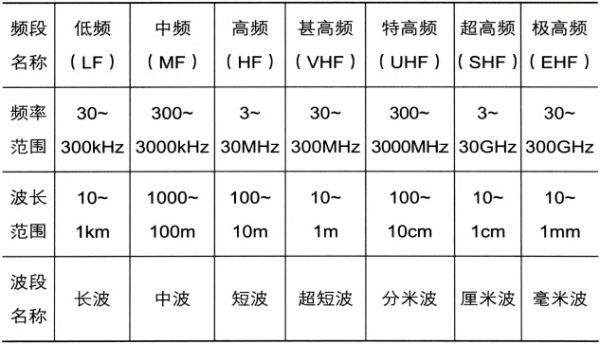
\includegraphics[width=0.7\linewidth]{17}
	\caption{无线电波频段的划分}
	\label{fig:1}
\end{figure}

\begin{figure}[htbp]
	\centering
	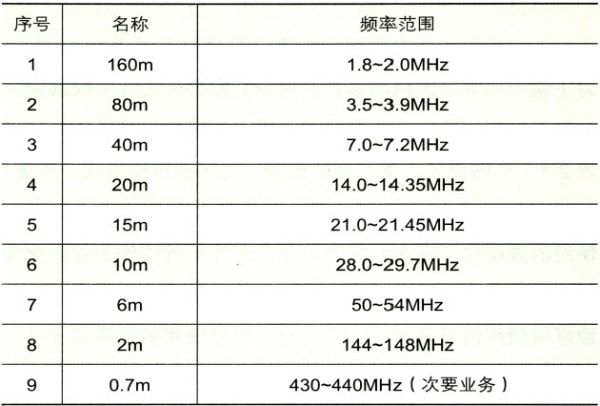
\includegraphics[width=0.7\linewidth]{18}
	\caption{业余业务频段}
	\label{fig:1}
\end{figure}

\section{VHF/UHF手持业余电台}

手持业余电台又称为对讲机,它是一种小型的移动通信工具,如图2-2所示。手持业余电台的最大优点是携带方便,野外活动时可以将手持业余电台抓在手上或放入衣袋中,手持业余电台主要用于FM通信。

VHF(甚高频)是指频率从30~300MHz的无线电波,UHF(特高频)是指频率从300~3000MHz的无线电波。实际上某个VHF/UHF手持业余电台的工作频率范围只是甚高频或特高频整个频段的一部分。

手持业余电台多为VHF/UHF单频段电台,也有许多手持业余电台可以多频段通信。例如八重洲VX-7R手持业余电台可以在50MHz、144MHz、430MHz 3个业余频段上通信。

由于受到体积的限制,手持业余电台不能提供较大的输出功率,手持业余电台所配的橡胶天线效率很低(见图2-3),这些因素使得手持业余电台的通信距离很有限,开阔地的通话距离为几千米。

\begin{figure}[htbp]
	\centering
	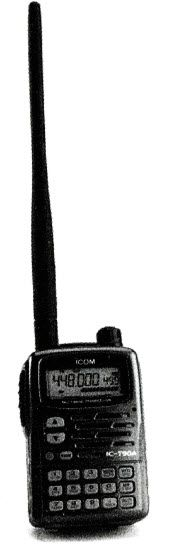
\includegraphics[width=0.7\linewidth]{19}
	\caption{FM手持业余电台}
	\label{fig:1}
\end{figure}

\begin{figure}[htbp]
	\centering
	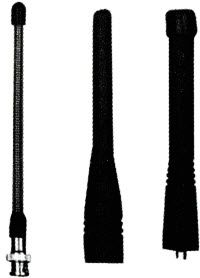
\includegraphics[width=0.7\linewidth]{20}
	\caption{螺旋橡胶天线}
	\label{fig:1}
\end{figure}

VHF/UHF波段手持业余电台设备的价格低廉,可选范围大。VHF/UHF波段又是爱好者的“入门波段”,世界上大多数爱好者都活跃在这个波段上。

\section{VHF/UHF车载业余电台}

车载业余电台是专门为汽车和其他交通工具设计制造的移动通信设备,车载业余电台仅能在业余频段发射信号。车载业余电台设计紧凑,外壳坚固结实,结构耐冲击和震动。电台大小一般按汽车收放机的大小标准设计,主操作通过前面板进行,较先进的机型还采用分离式面板的安装形式,方便在车内狭小的空间内安装。图2-4所示为一部八重洲双段车载业余电台。车载业余电台为我们带来驾驶车辆以外的另一种感受,利用车里的业余无线电设备进行通联,可以体验野外通信的乐趣。图2-5所示为一部车载业余电台在车内的安装位置。

\begin{figure}[htbp]
	\centering
	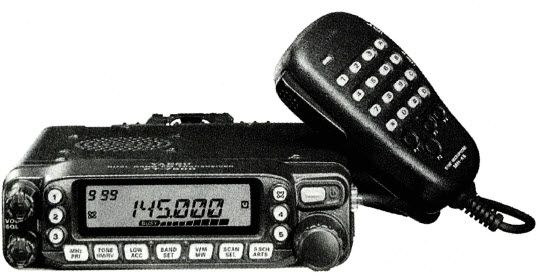
\includegraphics[width=0.7\linewidth]{21}
	\caption{八重洲FT-7800R VHF/UHF双段车载业余电台}
	\label{fig:1}
\end{figure}

\begin{figure}[htbp]
	\centering
	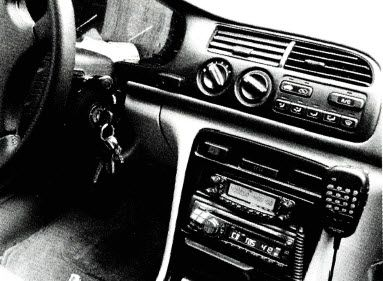
\includegraphics[width=0.7\linewidth]{22}
	\caption{车载业余电台安装的位置}
	\label{fig:1}
\end{figure}

车载业余电台具有较大的输出功率。在进行FM通信时,大功率能够通联更远的距离。但是,业余电台选用设备的最大输出功率不得超过无线电管理部门核发的《电台执照》所规定的功率。当然,车载业余电台也可以放在室内使用,接上电源和室外天线,它就是一部基地电台了。

在移动通信中,由于电台位置不断变化,为保证通信质量,一般要求移动电台及基地台天线在水平面内无方向性,并且采用垂直极化方式。我们通常看到工作在VHF/UHF频段的手持业余电台、车载业余电台、中继台都使用了各种形式的垂直极化无指向性天线。

车载天线(见图2-6)有吸盘天线和夹边天线两种。车载天线在结构上有1/4波长天线、1/2波长天线、5/8波长天线等形式。一般情况下天线越长,其增益也越高。若通信范围主要是在市区通过中继台进行通联,则可以选择增益较低的短天线。当用于郊外车辆间远距离联络时,宜选用高增益的长天线。由于高度的限制,加上车辆高速行驶时会遇到很大的风阻,所以车载天线的尺寸要依照工作频段采用不同的设计。

\begin{figure}[htbp]
	\centering
	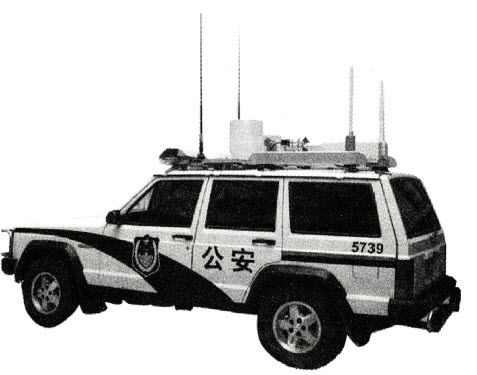
\includegraphics[width=0.7\linewidth]{23}
	\caption{车载天线}
	\label{fig:1}
\end{figure}

车载天线大多数是VHF/UHF双频段天线,这样只要一根天线就可以同时进行VHF频段和UHF频段的发射和接收。一般车载天线都是采用垂直极化方式,这种天线在水平方向上是均匀辐射的,这可以让我们在驾驶中不需要时刻想着天线的方向。图2-7所示是平面接地(GP)天线的立体方向图,这是一种典型的垂直极化全向天线。

\begin{figure}[htbp]
	\centering
	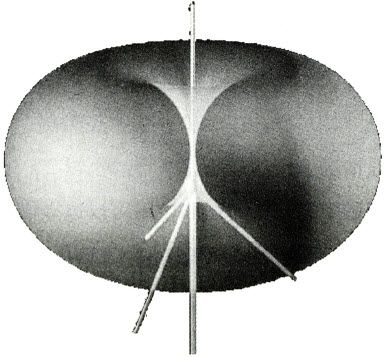
\includegraphics[width=0.7\linewidth]{24}
	\caption{GP天线方向图类似苹果形状}
	\label{fig:1}
\end{figure}

\section{短波业余电台}

短波(HF)业余电台是指发射频率在1.5~30MHz之间各业余频段的电台设备。图2-8所示为一部IC-718短波业余电台。短波业余电台的优点之一就是不需要很大的发射功率就能实现远距离通信。短波业余电台的输出功率通常为100W,在传播条件良好的情况下,这个功率可以进行全球范围的通信。

\begin{figure}[htbp]
	\centering
	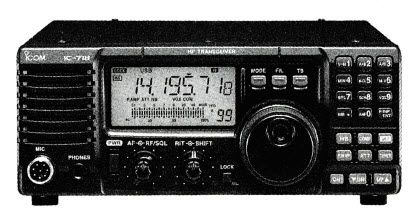
\includegraphics[width=0.7\linewidth]{25}
	\caption{ICOM IC-718短波业余电台}
	\label{fig:1}
\end{figure}

短波波段是比较常用的业余无线电波段,在这个波段上,业余无线电爱好者可以使用多种通信模式,其中包括:

\begin{itemize}
	\item SSB—单边带语音模式;
	\item CW—电报模式;
	\item AM—调幅语音模式;
	\item FM—调频语音模式;
	\item RTTY—无线电电传模式;
	\item SSTV—慢扫描电视模式。
\end{itemize}

目前,有些制造厂商设计出了HF/VHF/UHF多波段、多模式业余电台,发射频率范围可达1.9~440MHz间的各业余频率。我们将这类电台称作全波段电台,它是目前非常流行、畅销的电台,如图2-9所示。全波段电台既可以作为移动台,也可以作为基地台。一些全波段电台还具有业余卫星通信等扩展功能。

\begin{figure}[htbp]
	\centering
	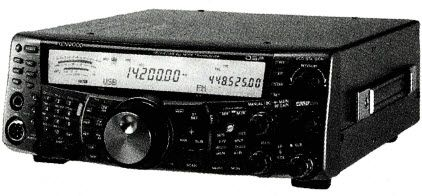
\includegraphics[width=0.7\linewidth]{26}
	\caption{建伍TS-2000 1.8~440MHz全波段电台}
	\label{fig:1}
\end{figure}

天线是无线电通信设备的耳目,天线的质量直接影响着电台通联的效果。电台通过天线向空中发射无线电波,同时通过天线从空中接收无线电信号,因此对电台来说,天线具有特别重要的作用。每部电台必须配备性能良好的天线才能实现好的通联效果。

短波业余电台常用的天线有半波偶极天线和八木天线。半波偶极天线是最容易制作的天线。它的结构非常简单,只需要将两根长度相同、总长度约为半波长的导线水平架设起来即可。偶极天线的长度由工作频率决定。以7MHz频段为例,它的波长λ≈42.85m。业余无线电爱好者通常将这个数字简称为40m,因此7MHz频段也称作40m波段。半波偶极天线两段导线的长度是1/4λ=10.7m,其外形如图2-10所示。

\begin{figure}[htbp]
	\centering
	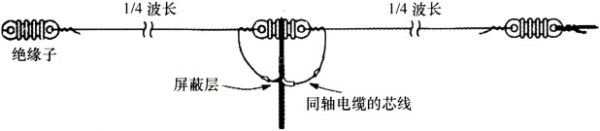
\includegraphics[width=0.7\linewidth]{27}
	\caption{水平半波偶极天线}
	\label{fig:1}
\end{figure}

八木天线是一种典型的定向天线。这种天线是由日本人八木秀次于1926年发明的,因此叫做八木天线。八木天线具有良好的方向性和高增益,配合转向器可以很好地工作在HF、VHF和UHF频段,图2-11所示为一个典型的短波八木天线。将多个八木天线组合起来,构成天线阵列,可以进一步提高八木天线的方向性,特别适合VHF/UHF频段远距离通联。

\begin{figure}[htbp]
	\centering
	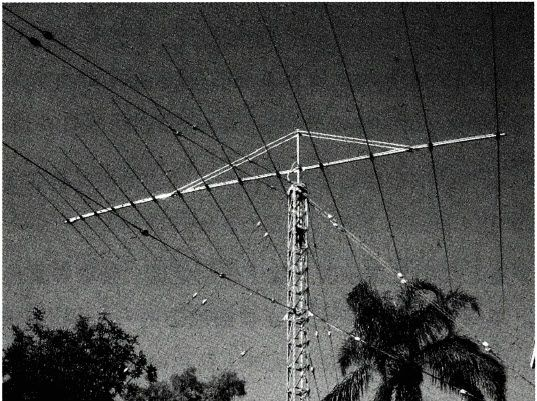
\includegraphics[width=0.7\linewidth]{28}
	\caption{HF频段14单元八木天线}
	\label{fig:1}
\end{figure}

\section{几个常用术语}

\subsection{频率范围}

为了合理地利用频率资源,保证用户之间不受干扰,无线电管理部门对手持业余电台的使用频率进行了划分,规定了不同行业使用的频率范围。常用的VHF、UHF业余频段一般是50~54MHz、144~148MHz和430~440MHz频段。业余无线电爱好者购买手持业余电台时首先要了解它的收、发频率范围是否包含144~148MHz、430~440MHz两个常用的业余频段,并且只能在业余频段发射。

\subsection{单段、双段}

单段电台只能在一个频段上收、发,双段电台可以工作在两个频段上。除单段、双段电台,有的对讲机制造商还设计出多频段电台。如八重洲FT-8900车载业余电台可以在29MHz、50MHz、144MHz、430MHz 4个业余频段上工作。

\subsection{单显、双显}

单显是指电台显示屏上显示一个信道、频率等其他指示图标。单显电台一般只能在当前频段上的一个信道(频率)上收、发。双显是指电台显示屏上显示两个信道、频率及指示图标。双显电台可以同时接收两个信道的信号,并能在其中任意一个信道上发射。

频段、显示方式  典型机型

单段单显     灵通LT-6100plus

单段双显     欧讯KG-689

双段单显     八重洲FT-7800

双段双显     八重洲FT-8800

\subsection{单工、双工}

单工通信是指在同一时刻信号只能单方向进行传输。单工电台的工作通常是以按键控制收、发的转换。当按下发射键时,发射机处于工作状态,接收机处于不工作状态;反之,松开发射按键时,接收机处于工作状态,发射机处于不工作状态。单工电台收、发交替工作,只能你说我听或者我说你听。

单工机根据频率使用情况,又分为同频单工机和异频单工机(半双工机)。同频单工机是指发射和接收都工作在同一频率上,它能有效地使用频率资源。异频单工机一般在有中转台的无线电通信系统中使用。现在很多单工机既能同频工作又能异频工作。

双工通信是指在同一时刻信号可以进行双向传输,和打电话一样,说话的同时也可以收听。双工电台的发射和接收分别工作在两个不同的频率上,所以也称为异频双工机。双工手持机大多在VHF频段和UHF频段上跨段工作。

\subsection{输出功率}

射频输出功率是决定通信距离的重要因素。功率越大,通信距离越远。手持式对讲机的输出功率一般在0.5~5W,车载业余电台的输出功率通常为5~50W。购买时可根据实际通信距离、《电台执照》的核定功率和《操作证书》等级来选择相应发射功率的电台设备。

\subsection{灵敏度}

灵敏度是指通信设备接收微弱信号的能力。灵敏度高的接收机能够收到较远电台微弱的信号。通常以输入信号电压的大小来表示灵敏度,单位是微伏(μV),这个数值越小,表示接收机的灵敏度越高。

\subsection{FM和SSB}

FM和SSB是业余无线电通信中最常用的两种语音通信模式。我们可以通过特定的电路,来改变无线电信号的幅度或频率,以便承载声音、图像信息。如果我们让信号的频率随语音发生改变,这就是调频,即FM。

FM通信的最大优点是它的接收性能良好,信号清晰,几乎没有噪声,机器调整也比较简单。现在,手持业余电台和车载业余电台多采用FM调频模式。

SSB是单边带语音通信的缩写。一般通信系统中,载波经音频信号调制后,包含载波和上、下两个边带信号,这两个边带含有相同的信息。为了提高通信效率和节约通信频带,我们可以通过单边带电路,将载波和另一边带去除掉,只发送一个边带,这种通信方式就称为单边带通信。单边带电台与调幅、调频电台相比,具有节省频谱、节约功率等优点,特别适合远距离通信。在短波(HF)段上一般都采用SSB通联。

\chapter{第一次通联}

引子
“CQ CQ CQ,这里是BY4RWT, BRAVO YANKEE FOUR ROMEO WHISKEY TANGO, BY4RWT呼叫……”

业余电台通话不能像打电话那样,想怎么说就怎么说。业余无线电通信有它特定的通话语言、通话规则和通信程序。要顺利地完成一次通联,业余无线电爱好者除了要具备基本的电台操作技能外,还要熟练掌握通信语言,了解业余通信基本程序,以保证通信中取得最佳的通联效果。

\section{通联前的准备}

\subsection{业余通信基本程序}

\subsubsection{呼叫}

呼叫前在你准备使用的频率上收听一会儿。业余频段上的电台较多,相互之间要避免干扰。如果听到频率上已经有电台在工作,则应更换频率呼叫。

为防止干扰,可以先问一声“这个频率上有人吗”,英语则用“Any body here”,如果听到有人回答,就应主动更换一个频率。

· 普遍呼叫

没有特定联络对象的主动呼叫称为普遍呼叫。听到普遍呼叫后的业余电台都可以回答。如BY4RWT普遍呼叫的程序是:

“CQ,CQ,CQ,这里是BY4RWT,BRAVO YANKEE FOUR ROMEO WHISKEY TANGO,BY4RWT呼叫,听到请回答……”

· 区域性呼叫

将联络对象限制在一定范围内的呼叫称为区域性呼叫。区域性呼叫程序与普遍呼叫程序基本一致,当听到其他电台在进行区域性呼叫而自己又不在被呼叫的范围内时不要应答。

如只呼叫中国电台:

“CQ BRAVO,CQ BRAVO,CQ BRAVO……”

呼叫不包括本国在内的远距离电台:

“CQ DX,CQ DX,CQ DX……”

· 插入呼叫

当两个电台正在联络,你想呼叫其中的一个,可以等他们讲完后呼叫。在有特殊情况时,可在双方谈话告一段落时插入呼叫。随便插入或打断别人的谈话,都是不礼貌的行为。

例如:“BY4RWT请求插入……”

\subsubsection{回答}

在听到某台呼叫,而自己属于被呼叫范围,你可以准备与其联络。回答的程序是:“BY4RWT,BRAVO YANKEE FOUR ROMEO WHISKEY TANGO,我是BG4RYN,BRAVO GOLF FOUR ROMEO YANKEE NOVEMBER,请回答。”

\subsubsection{沟通后的联络}

当双方已经相互收到对方的呼号后,就可以进行其他各项内容的交流。每次发信时可加上“听到”、“明白”、“抄收”、“Roger”等用语,表示刚才对方发过来的信息已全部抄收。讲话结束时要加上“完毕”、“请讲”、“请过来”、“Over”等用语,让对方知道自己已经转为收听状态。例如:

“听到。BG4RYN,这里是BY4RWT,很高兴在空中见面,您的信号是59。我叫孙倩,我的位置在南京五塘中学。BG4RYN,这里是BY4RWT,请讲。”

“Roger,BY4RWT,我是BG4RYN,你过来的信号也是59。我姓任,我在中央门附近。BY4RWT,我是BG4RYN,Over。”

\subsubsection{结束联络}

双方完成联络后,要以明确的语言结束联络,以便其他电台知道该频率已经空出。例如:

“……谢谢今天良好的联络,希望再次见到你。BG4RYN,这里是BY4RWT。73,再见!

“BY4RWT,我是BG4RYN。73,再见!

一般情况下,业余通信时还可以介绍自己的姓名、电台所在的地理位置、交换QSL卡片的地址、交换所用设备和天气情况等。每次通信内容应力求简洁,不要长谈。在业余电台上漫无边际的长时间聊天甚至调笑是违反业余电台有关规定的行为。

一次成功的联络,至少应包括下面3个内容:

\begin{itemize}
	\item 双方都正确地抄收了对方的呼号;
	\item 交换信号报告;
	\item 将这次的联络情况正确地记录在电台日记上。
\end{itemize}

通信程序举例如表3-1所示。

\begin{figure}[htbp]
	\centering
	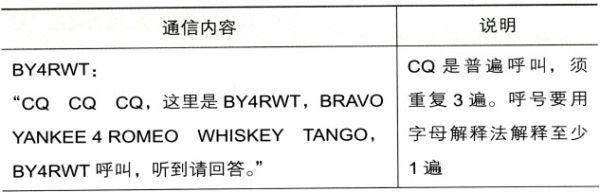
\includegraphics[width=0.7\linewidth]{29}
	\caption{}
	\label{fig:1}
\end{figure}

\begin{figure}[htbp]
	\centering
	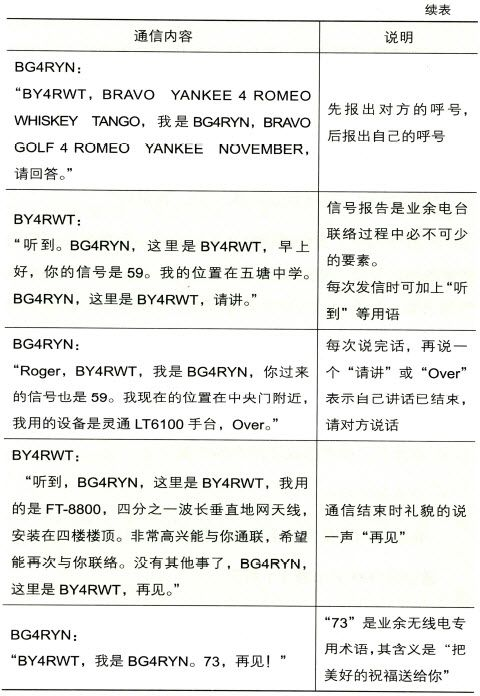
\includegraphics[width=0.7\linewidth]{30}
	\caption{}
	\label{fig:1}
\end{figure}

\subsection{呼号}

虽然我们找到了宽广的“跑道”,了解了各不相同的分区,但在纷杂的无线电信号中怎样才能找到自己需要的某个业余电台呢?这就需要我们熟悉它们的名字——业余电台的呼号。

每一个业余电台呼号都是唯一的,只代表一个特定的电台,它们之间是没有也不允许有“同名同姓”的。

工业和信息化部于2012年颁布的《业余无线电台管理办法》(见附录14),对中华人民共和国境内(不包括港澳台地区)业余电台呼号的申请、分配、指配、使用、撤销等相关管理做了详尽的规定与说明。

业余电台呼号的组成有4个部分:第1部分为代表国家的字母前缀,由“B”表示;第2部分为电台种类,由一位英文字母表示;第1部分和第2部分常合并称之为呼号前缀;第3部分为本国业余电台分区,即电台所在地的分区数,由一位阿拉伯数字表示;第4部分为后缀,以区分同一分区内不同的业余电台,由不超过4位的字母或字母和数字的组合表示。我国规定只具备收信功能的业余无线电台不指配业余无线电台呼号。有些国家的收信台后缀以4~5位阿拉伯数字表示。

字母前缀(Prefix)位于呼号的最前面。国际上一般由1~2个英文字母或字母和数字组合而成。例如:B、W、A5、3X等。它是由各国根据国际电信联盟排定的“国际呼号序列分配表”划分给业余电台使用的,所以前缀是每个业余电台所属国家或地区的标志。当你听清了一个呼号的前缀后,可以从“国际呼号序列分配表”查出这个电台所属国家或地区。例如前面列出的4个呼号冠字就分别属于中国、美国、不丹和几内亚。

ITU划分给中国的呼号前缀共有3个系列,即BAA~BZZ,XSA~XSZ,3HA~3UZ。任何种类业务的中国无线电台,其呼号前缀都必须在以上3个系列的字符组合范围内。我国规定业余电台使用以字母B开头的一个系列。由于历史的原因,我国香港和澳门两地区目前使用的业余呼号前缀分别是VR2和XX9,台湾地区使用BV、BO、BW、BX等前缀。随着社会的进步和科学技术的发展,目前有不少国家和地区向南极派出科考队和在南极建立了科考站,业余电台也随之进入了南极地区,这些国家和地区的爱好者所建立的业余电台,已分布在南极的四面八方,目前中国也已在南极建立了4个科考站,我们殷切地希望中国HAM能早日在自己的科考站内发出业余无线电信号有些呼号还包含有对业余电台性质等的说明。我国的业余电台呼号中第二部分的一个字母即属此例,用以代表电台种类。具体表示方法见表1-4。

\begin{figure}[htbp]
	\centering
	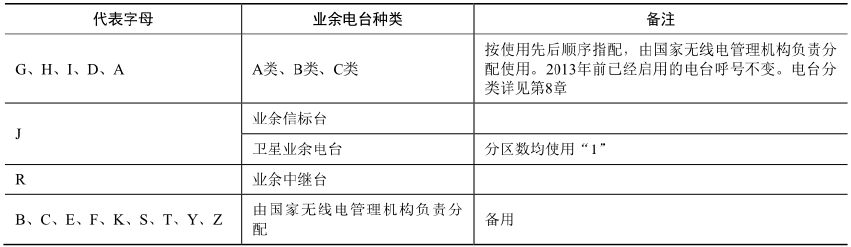
\includegraphics[width=0.7\linewidth]{83}
	\caption{业余电台种类及代号一览表}
	\label{fig:1}
\end{figure}

呼号的第3部分是“国内业余分区”,用一位数字(Number)表示。国际上业余电台呼号中间的数字一般也是这样,你可以根据其分区数字了解到这个电台位于该国家的哪个地区,从而使你的联络更具针对性。呼号中的数字“零”应读作“Zero”,为不和字母“O”混淆,书写一般以“0 ”表示。

呼号的最后一部分是后缀(Suffix),表示这个电台在本分区内的编码。由不超过4位的字母或者字母和数字的组合表示,其中最后一位应为字母。这些字母或数字的排列原则由各国自行决定,一般以领取执照的先后为序。有的国家的呼号后缀含有特定的意义,如日本的呼号后缀第一个字母用“Y”或“Z”代表集体电台。我国幅员辽阔,所以后缀第一个字母还代表了同一分区内不同的省、直辖市、自治区。比如:4AA~4HZZ为上海、4QA~4XZZ为江苏范围内的业余电台呼号后缀……,以上几个部分合起来便组成了电台自己的“名字”。

中华人民共和国境内(不包括香港、澳门、台湾地区)各省、自治区、直辖市业余电台的呼号双字母、三字母后缀分配如表1-5所示。此表中未列入的呼号后缀由国家无线电管理机构负责分配。一位、四位或者带有数字的呼号后缀留作备用。根据《业余无线电台管理办法》,我国业余电台呼号均由国家无线电管理机构负责分配。

\begin{figure}[htbp]
	\centering
	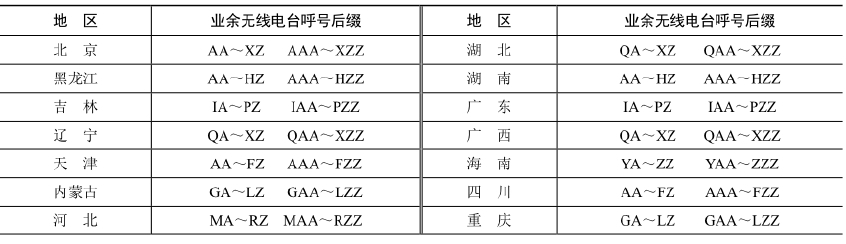
\includegraphics[width=0.7\linewidth]{84}
	\caption{各省、自治区、直辖市(不包括香港、澳门、台湾地区)业余电台呼号后缀分配表}
	\label{fig:1}
\end{figure}

\begin{figure}[htbp]
	\centering
	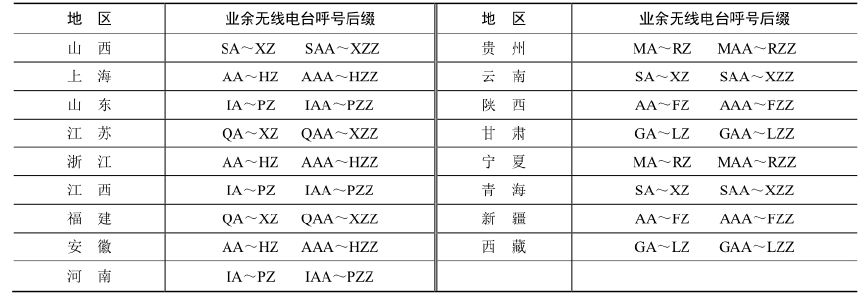
\includegraphics[width=0.7\linewidth]{85}
	\caption{各省、自治区、直辖市(不包括香港、澳门、台湾地区)业余电台呼号后缀分配表}
	\label{fig:1}
\end{figure}

说明:1.无线电通信业务缩略语QOA~QUZ及SOS、XXX、TTT等可能与遇险信号或类似性质的其他信号混淆的字母组合不用作呼号后缀。
2.BS7H为黄岩岛业余无线电台呼号。
表1-5说明中的第1条是按照国际电信联盟的规定而设,因为这些字母的组合另有特定的含义,如用于呼号会引起混乱,它们是:①可能与遇险信号或其他类似性质信号相混淆的组合,比如“SOS”是遇险求信号,“XXX”是紧急信号,“TTT”是安全信号等;②留供无线电通信业务用缩语(详见第2章)的组合,比如“Q简语”等。
在通信中我们还常遇到这样的情况:在一个符合上述规律的呼号后面还加有一个“/”符号(在这里常读作Portable或slash)以及若干字符,这是为了进一步说明这个电台的一些情况而加的附注。例如,呼号后面加“/M”(读作Portable mobile或只读Mobile)、“/AM”“/MM”分别代表该台在陆地上、在空中、在海上移动;“/QRP”是表示发信机输出功率在5W以下的小功率电台;“/P”表示便携电台等。
在设台地以外的地方操作时,还应该在呼号的前面加所在地呼号前缀、分区数,并在其之后加斜线号。例如“KH6/W6KZ”表示美国6区爱好者在夏威夷发射。我国法规要求,业余无线电台在设台地以外的地点进行异地发射操作时,应使用“字母B、操作地业余无线电台分区号、斜线符号‘/’、本人业余无线电台呼号”格式的呼号。例如设台地在江苏省的业余电台BA4RC到北京操作,应使用“B1/BA4RC”呼号。
也有不少将斜线符号和所在地分区数放在本台呼号后面使用的地方,如“BV2B/1”“RX9TL/9”“JG3AY/3”等,不过这类“后置斜线分区数”的表示方法仅限于移动范围在同一呼号前缀区内可以使用,且这种格式的呼号不为我国现行管理办法所允许,这是我国爱好者必须加以注意的。
根据我国管理规定,一个爱好者或一个单位在设置业余无线电台并取得电台执照的同时,就可以取得一个业余电台呼号。当电台类别发生变化时(如先设A类电台,后来又设立B类电台)呼号不变。
无线电管理机构依法注销业余无线电台执照时该电台呼号也将被同时注销。被注销的呼号在注销5年后可以另行指配。但如果该台被注销后1年内,设置人又申请设台的,无线电管理机构应当指配原业余无线电台呼号。如果电台执照被依法注销后1年内,设置人在其他省、自治区、直辖市申请设台的,还可以申请使用原业余无线电台呼号,但应当事先征得指配原呼号的无线电管理机构的书面同意。


就像我们每个人有不同的姓名一样,业余电台的呼号是用来识别电台身份的一个代号。每个业余电台呼号由3个部分组成:前缀、业余分区、后缀。

前缀位于呼号的最前面,由1~2个英文字母或字母和数字组合而成,例如呼号BY4RWT、W3EP中的BY、W。它是由各国根据国际电信联盟排定的“国际呼号系列划分表”划分给业余电台使用的,所以前缀是每个业余电台所属国家或地区的标志。当你听清了一个呼号的前缀后,可以从“国际呼号系列划分表”查出这个电台的国籍。

有些呼号还包含有对业余电台性质的说明。我国的业余电台呼号中的第二个字母即属此例,如BA表示持有一级《操作证书》的个人业余电台,BY代表集体台,BT表示为某个重大活动临时设立的特设电台。

呼号的第二部分是“国内业余分区”,用一位数字表示。你可以根据其分区情况了解到这个电台位于该国家的哪个地区,我国的业余电台分区见表3-2。

表3-2 我国业余电台分区表

\begin{figure}[htbp]
	\centering
	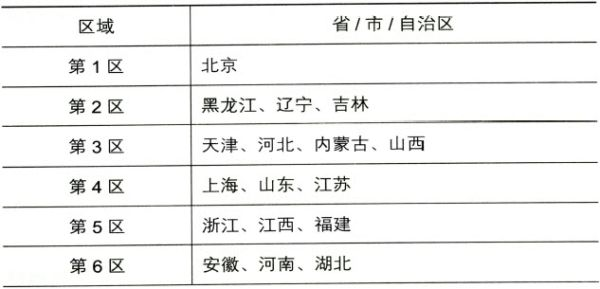
\includegraphics[width=0.7\linewidth]{31}
	\caption{}
	\label{fig:1}
\end{figure}

\begin{figure}[htbp]
	\centering
	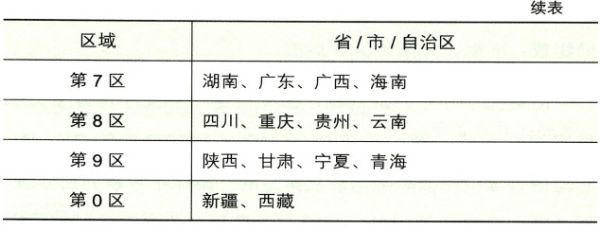
\includegraphics[width=0.7\linewidth]{32}
	\caption{}
	\label{fig:1}
\end{figure}

呼号的最后一部分是后缀,这是电台自己特有的名字。后缀一般由1~3个字母组成。如清华大学业余电台的呼号是BY1QH,前缀中的字母B代表中国,Y代表集体电台,1表示业余分区在第1区(即北京市),QH为呼号的后缀。世界各国遵照国际电信联盟(ITU)有关呼号划分的规定,制定出本国字母的排列原则,从而保证了电台呼号的唯一性。我国业余电台的呼号由各省(市、自治区)无线电管理机构分配。

\subsection{信号报告}

信号报告是业余无线电通信中最基本的技术数据,准确的信号报告可使双方了解自己收、发信设备的效率及电波的传播情况。业余电台的信号报告由信号可辨度(R)、信号强度(S)以及信号音调(T)3部分组成,所以信号报告也常称为“RST”。在语言通信中,只报告前2项;在电报、电传及其他一些数字通信中应报告全部3项。

\subsubsection{信号可辨度}

信号可辨度“R”位于信号报告的第一位,共分5级,用1~5中的一位数字表示,如表3-3所示。信号可辨程度的判断依靠主观经验。在通常情况下,对于能顺利进行联络的信号总是给予最高等级——5的报告。

表3-3 信号可辨度分级表

\begin{figure}[htbp]
	\centering
	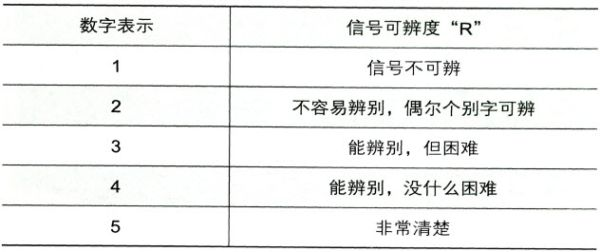
\includegraphics[width=0.7\linewidth]{33}
	\caption{}
	\label{fig:1}
\end{figure}

\subsubsection{信号强度}

信号强度“S”位于信号报告的第二位,共分9个级别,用1~9中的一位数字表示,如表3-4所示。信号强度报告可以借助收、发信机面板上的仪表指示判读,见图3-2。有些收信机没有“S”表,则应参照定级标准依靠主观判断。

表3-4 信号强度分级表

\begin{figure}[htbp]
	\centering
	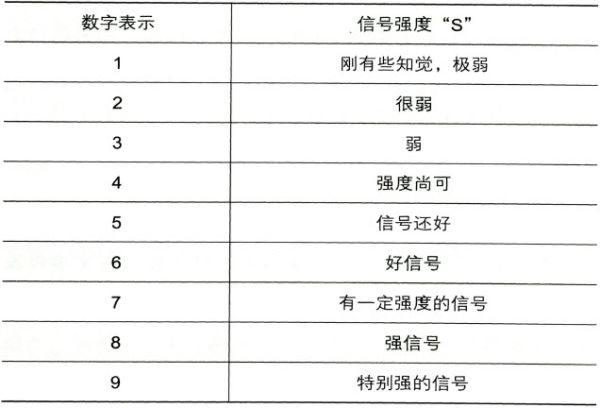
\includegraphics[width=0.7\linewidth]{34}
	\caption{}
	\label{fig:1}
\end{figure}

\begin{figure}[htbp]
	\centering
	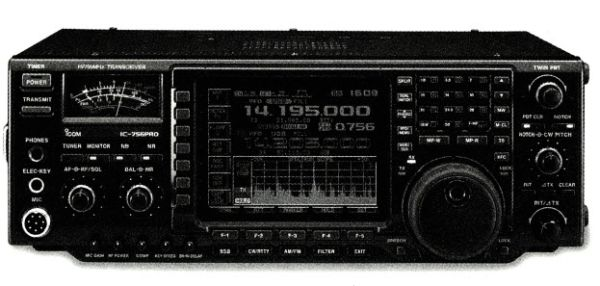
\includegraphics[width=0.7\linewidth]{35}
	\caption{IC-756PRO电台左上角“S”表可指示信号强度}
	\label{fig:1}
\end{figure}

信号音调“T”位于信号报告的第三位,也用1~9中的一位数字表示。在报告信号时,代表“RST”的3位数字应同时报出,因此,对于好信号的报告,在语言通信中就是“59”,而在电报、电传等通信中的报告就是“599”了。

在VHF/UHF波段使用FM调频方式通话,当信号强度大于一定水平时,接收机听到的声音都很清楚,如果电台上没有信号强度指示,凭听觉很难对信号强度进行评估,这种情况下的信号报告只能粗略估计了。

\subsection{英文字母解释法}

在日常生活中,人们有时需要对某些汉字进行解释,如“木子李”、“弓长张”。语言通信中,由于部分英文字母发音相近,如字母S和X、M和N,另外信号在传播过程中受到干扰等原因,我们对有些字母分辨变得非常困难。为解决这个问题,人们约定用一些大家熟悉的单词来代表、解释相应的字母。根据国际电信联盟(ITU)的规定,业余无线电通信中采用国际民航组织(ICAO)使用的解释法作为“标准解释法”。此外还常用一些人们熟悉的地名、人名等来解释。

例如:“CQ CQ CQ,这里是BA4RM,BRAVO ALPHA FOUR ROMEO MIKE呼叫,听到请回答。”

英文字母解释法是业余无线电通信中必须掌握的基本知识。电台呼号、姓名、地址等许多信息的说明都需用到英文字母解释法,如表3-5所示。

表3-5 英文字母解释法

\begin{figure}[htbp]
	\centering
	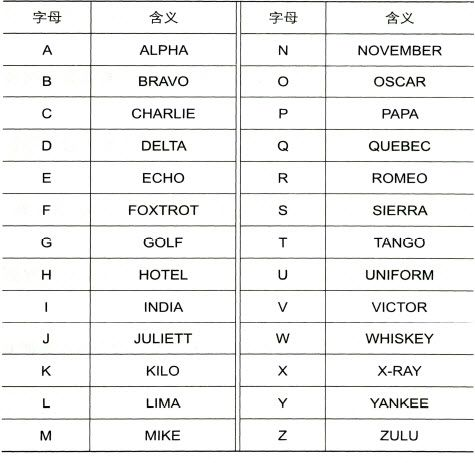
\includegraphics[width=0.7\linewidth]{36}
	\caption{}
	\label{fig:1}
\end{figure}

\section{开始通联}

知道业余电台通信程序、电台呼号、英文字母解释法等基本内容后,便可以开始通联了。第一次通联总是令人紧张、兴奋的。打开电台后,不要急于通联,先仔细收听其他爱好者的通联,熟悉通联步骤、通联用语,掌握电台频率、功率的调整方法,没有问题后,再拿起话筒开始通联。

与其他爱好者建立通联有两种方法:一是自己呼叫CQ,等待其他电台的回答;二是回答正在呼叫CQ的其他电台。

\subsection{呼叫}

在开始呼叫CQ之前,首先要寻找一个未被其他火腿使用的空闲频率,养成呼叫之前先监听的好习惯。开机收听一会儿后,可以询问一次:“这个频率有人使用吗?这里是BA4RM。”确认该频率上没有人使用,再进行呼叫。呼叫CQ之后,如果没有人回答,可以稍等片刻,再次呼叫。如果呼叫三四遍后,一直没有人回答,可能这个频率上确实没有人收听,这时,你可以更换其他频点试试。

用车载业余电台进行呼叫时,应在自己的呼号后面加上“/所在的分区”或“/M”。比如BA4RM驾驶汽车来到北京,汽车停在某处呼叫:

“CQ CQ CQ,这里是BA4RM/1,BRAVO ALPHA FOUR ROMEO MIKE PORTABLE ONE呼叫,请回答。”

操作者报告自己的呼号(BA4RM/1)之后,又用字母解释法再次报告一遍,是让对方听清楚呼号,以防抄错,其中的斜线读作“Portable”。

业余电台操作首先要学会使用话筒。在通话过程中,手持话筒姿势要端正,一般用拇指或食指按压收、发控制键(PTT),嘴离话筒不要太远,大约10cm的距离为宜。

由于业余电台通联多为单工方式,说话和收听不能同时进行,而是通过PTT键控制说话和收听的转换。说话时按下PTT键,说完就立即松开,听对方讲话。别人呼叫时,自己不能随便按下PTT键说话,否则两人都无法听到对方的声音。

业余电台通联中,通话内容要简洁,语速平稳,语音清晰,语言礼貌、规范。无论何时何地进行通联,都要记住你代表的是一个群体,是整个业余无线电界的形象。

\subsection{移动通信的乐趣}

在汽车或其他交通工具上装备无线电通信设备,人们可以在移动中进行通信,这种通信方式叫做移动通信。移动通信方式灵活机动,能保持随时随地通联。现在,移动通信已广泛应用于各个行业及人们的日常生活当中。
业余电台联络方式可分为直发通信和中继通信。直发通信是指两电台直接进行通联,不经过中继台或其他电台转发。通常直发通信电台的发射频率和接收频率设置在同一个频点上,操作者通过PTT键来切换收、发状态。与邻近电台通联一般就选用这种通信方式。当然,这种模式也可以用于车队,让所有车载业余电台工作在相同的频率上,构成一个专门的移动通信网络,这也是最简单的一种组网方式了,如图3-3所示。需要注意的是,车载业余电台频率设置要严格遵守当地无线电管理部门的有关规定。

\begin{figure}[htbp]
	\centering
	\includegraphics[width=0.7\linewidth]{37}
	\caption{F1是移动通信网络的固定频点}
	\label{fig:1}
\end{figure}

目前汽车上装备的通信设备大多数是VHF(144MHz)和UHF(430MHz)频段的车载业余电台。VHF和UHF频段的电波以视距传播为主,沿地面传播距离一般在50km以内。考虑到车载业余电台的设置条件和移动通信的不稳定性,实际通信距离还会缩短。在平坦的开阔地段车载业余电台之间的通信距离一般在5~15km,所以,若想实现与较远电台的联络,还要充分利用地形,灵活掌握通联时机。

一般来说,当汽车行驶到开阔地或地势较高的地段时,往往可以呼叫到较远的联络对象。当车辆进入山谷或高楼林立的市区,通联常常中断。在高速公路上,汽车行驶到信号较弱的地区,会出现信号周期性消失的现象,工作频率越高,汽车速度越快,信号断续得就越频繁。若这种影响使得车载业余电台无法通联时,可降低汽车速度或将车辆停在信号较强的地方完成联络。

移动通信中的电波传播非常复杂,特别是车辆进入丘陵地带和城市中,山峰或高楼对电波传播的阻挡、反射,使得到达车载业余电台的信号时大时小,联络时通时断。这种情况下,电台操作者可以采取短呼叫、勤呼叫的方法进行联络,一旦信号好时就快速完成通联。若两台无法直接联络,可考虑通过其他电台转发或中继台完成通联。

\subsection{中继通信}

业余电台依靠中继台(Repeater)对电波的转发而建立通信称为中继通信,如图3-4所示。中继台是一种自动接力设备,当它收到信号以后,便启动发射机,把信号转发出去。由于中继台具有很好的接收性能和比较大的发射功率,所以通过它的转发,手持业余电台或车载业余电台的通信距离可以增加到几十千米甚至几百千米。

\begin{figure}[htbp]
	\centering
	\includegraphics[width=0.7\linewidth]{38}
	\caption{中继通信}
	\label{fig:1}
\end{figure}

\subsubsection{上行频率和下行频率}

中继台由一个发射机、一个接收机和一副天线组成,因此它与一般电台没有本质的区别。中继台的最大特点是接收机与发射机使用不同的频率。习惯上,把中继台的接收频率称为上行频率,发射频率称为下行频率。上行频率和下行频率的差值,叫做频差。频差的大小各地不尽相同,推荐标准是:UHF频段5MHz,VHF频段0.6MHz。

在使用中继台之前,必须将自己电台的发射频率和接收频率设置为两个不同的值。例如中继台上行频率是434.225MHz,下行频率是439.225MHz,则我们应该把439.225MHz设置成为自己的接收频率,把434.225MHz设置为自己的发射频率;或者在439.225MHz的基础上设置5MHz的频差。

\subsubsection{亚音}

“亚音”是“连续音调静噪控制系统(CTCSS)”或“亚音频静噪控制系统”的俗称。使用中继台通常都要求操作者发送亚音,中继台只有接收到你的亚音信号,才允许使用它。启用亚音功能并不是要限制爱好者使用中继台,而是为了防止外界干扰。如果没有亚音,任何无关的信号都有可能触发中继台。

实际上,亚音是一个低频信号,亚音的频率比我们耳朵可以听到的最低音频还要低,但中继台可以识别它。那么如何向中继台发送亚音呢?这就需要启动电台的CTCSS功能。启动CTCSS功能之后,电台会将亚音信号附加在正常的音频信号上一同发射出去。目前大部分VHF/UHF电台都有CTCSS功能。常用的亚音频率见表3-6。

表3-6 常用的亚音频率(Hz)

\begin{figure}[htbp]
	\centering
	\includegraphics[width=0.7\linewidth]{39}
	\caption{中继通信}
	\label{fig:1}
\end{figure}

若中继台CTCSS亚音频率设置为88.5Hz,则你使用的电台亚音也必须设置在88.5Hz。当然,只需让发射信号带有亚音就行了,接收可以不用设置。

\subsubsection{中继操作}

· “上”中继

当一切设置就绪,在频率空闲的情况下,应先测试能否“上”中继。拿起话筒说:“BA4AAA”以便引起别人注意。松开发射键(PTT)后,你会收到一个很短的没有调制的载频信号,手持台发出“嚓”的一声,这说明中继台处于正常的工作状态。如果有人想与你联络的话,他会呼叫你。只要通信各方都能“上”中继,就能建立中继通信。

· 报呼号

业余电台在每次通信建立以及结束时,应当主动报出本台的完整呼号。如果你要呼叫某个人,可直接呼叫:“BA4BBB,我是BA4AAA”。不要在呼叫时省略自己的呼号,而让被叫电台回答你时再询问你是谁。如果只是两个人在中继台上通话,可以不报对方的呼号,只报自己的呼号即可。

· 留有间隙

不要在对方松开PTT键时立即按键发射,每次发信前留有一定的间隙,可使其他人利用这一短暂的时间插入。如果你在通话中听到他人要求插入,应给予答复。不答复或答复却不给他发信的权力都是不礼貌的。

· 移动台优先

中继台通常是供直接联络有困难的爱好者使用的。在中继台繁忙的时候,应优先让移动台使用。移动台往往在某个地区才能打开中继台,移动到其他地区可能就无法使用中继。每次通联时间应尽可能短,以便让更多的爱好者使用中继台。如果能直接通联的话,就不要使用中继台。

我国许多城市都建立了2m和70cm频段的中继台。在你出差、旅游时,可以上网查找沿途城市中继台的频率,了解当地中继台的使用方法。

\section{QSL卡片}

QSL卡片是业余电台之间确认互相联络或收听报告的凭证,图3-6和图3-7所示分别为QSL卡片的正、反面。它多以14cm×9cm或15cm×10cm的硬质纸卡印制而成。每个业余电台都应有自己的QSL卡片,以便与世界各地的电台联络后互相交换。QSL卡片不仅是在一定程度上反映每个电台通信能力的标志,而且还是业余电台向有关机构申请各类奖状、证书的凭证。

\begin{figure}[htbp]
	\centering
	\includegraphics[width=0.7\linewidth]{40}
	\caption{QSL卡片正面}
	\label{fig:1}
\end{figure}

\begin{figure}[htbp]
	\centering
	\includegraphics[width=0.7\linewidth]{41}
	\caption{QSL卡片反面}
	\label{fig:1}
\end{figure}

来自世界各地的QSL卡片都填有对本台信号的收听情况及有关的各类数据,所以它又是研究、改进电台设备极好的技术资料。业余无线电爱好者们都以能收集到世界各地,尤其是那些业余电台稀少地区的QSL卡片为最大的乐趣。

\subsection{QSL卡片上的内容}

\begin{itemize}
	\item 醒目的本台呼号。
	\item 中国无线电运动协会会徽图案。
	\item CQ分区、ITU分区。
	\item 发至何台。
	\item 确认双方的联络或收听台的报告。
	\item 联络的时间。
	\item 联络时所用的频率。
	\item 联络时所用的操作方式。
	\item 对方的信号情况,即RST报告。
	\item 本台所在地的中英文详细地址。
	\item 集体台应有本台的中英文台名。
	\item 操作者签名。
\end{itemize}

除以上必须包括的内容外,许多爱好者的QSL卡片上还印有介绍自己设备、天气情况及附言等的栏目。

\subsection{正确填写QSL卡片}

QSL卡片既然是一种联络凭证,填写时就必须如实、认真,字体应清楚、正规,对方呼号中的英文字母最好使用大写印刷体,时间一律使用世界协调时(UTC),数字“0”应写成“Ø”。签名时应把全名写上,寄给国内的用汉字,寄给国外的用汉语拼音。在图3-7所示的示例中,如果发出的是确认联络的卡片,则在“OUR QSO”一栏中打上勾;如果是发给某收信台,确认收听报告的卡片,只要在“YOUR REPORT”一栏前画上勾。收信台卡片中“CLG/WKD”一栏,如果听到某台正在呼叫,也可以填写收听报告卡片,只需将这一栏的“WKD”划去,留下“CLG”并将你听到的呼叫内容填上即可,如呼叫“CQ”即填写“CQ”,如呼叫“BY1PK”就填写“BY1PK”。任何项目都不能填错,一旦填错,必须另换一张重新填写。涂改过的QSL卡片一律无效。

\subsection{QSL卡片的交换}

交换QSL卡片通常采用直接交换或经卡片管理局交换的方式。

\subsubsection{直接交换}

直接交换就是将卡片按对方的通信地址直接邮寄,因此在联络时应将对方的详细地址询问清楚。同样,如果希望对方也将卡片直接寄给自己,也应在联络时将自己的详细地址报给对方。

寄往国外的信封书写格式与我们平时使用的国内信函不一样。国际信函的收信人姓名、地址写在右下方,寄信人的姓名、地址写在左上角或信封的背面。姓名、地址的书写顺序也正好与国内信函相反,姓名在地址的前面,地址由小到大排列。图3-8所示是南京市五塘中学寄往美国的信封,右下角4行的内容从上到下分别为收信人姓名、门牌号及街道名、城市名及州名的缩写和邮政编码、国名。

\begin{figure}[htbp]
	\centering
	\includegraphics[width=0.7\linewidth]{42}
	\caption{寄往国外的信封书写格式}
	\label{fig:1}
\end{figure}

\subsubsection{经过卡片管理局交换}

很多国家和地区都设有全国性或地方性的卡片管理局,专门负责转寄国外爱好者的QSL卡片。通过管理局交换卡片比较方便,还可以节省邮资,但由于中转环节较多,收卡时间比较长。

寄发收听报告卡片的一般原则是只要听到对方信号,无论是呼叫还是联络,都可以向这个电台寄发收听报告卡片,当然,这要以听到对方的呼号为前提。没有听到呼号或从联络对方的呼叫中知道其呼号是不能寄发收听报告卡片的。

\subsection{QSL卡片的制作}

QSL卡片分为双面印刷和单面印刷两种。双面印刷的QSL卡片,一般在正面印有图案、照片和自己的呼号等,反面则为需要报告的各项内容。单面印刷的QSL卡片,就是把自己的呼号和要报告的内容都印在卡片的一面,这种卡片简单、明了,印刷成本较低,为不少爱好者所青睐。

除购买空白的QSL卡片或委托印刷厂印制外,还可以用黑白或彩色打印机打印卡片。每次打印之前,爱好者都可以临时设计一种新式样或者一张新图片,因此这种卡片是完全个性化的卡片。制作时选用250~300g的A4纸正好可以打印4张。所需的中国无线电运动协会会徽图案及QSL卡片模板可从网上下载(http://www.qslprinter.com)。

图3-9所示为2008年北京奥运会特设业余电台QSL卡片。

\begin{figure}[htbp]
	\centering
	\includegraphics[width=0.7\linewidth]{43}
	\caption{2008年北京奥运会特设业余电台QSL卡片}
	\label{fig:1}
\end{figure}

\section{电台日志}

电台日志(Station Log)是无线电爱好者在电台联络时,用来登记各种数据、资料以及联络情况的原始记录,它是业余电台唯一的工作记录,也是寄发QSL卡片的依据。

各国电台日志的内容大致相同。我国电台日志包括的内容有:日期、开始时间、结束时间、使用频率、对方呼号、操作方式、信号情况、内容摘要、QSL卡片的收发日期、签名。

填写电台日志和填写QSL卡片一样,时间一律使用协调世界时(UTC),呼号中的英文字母应使用大写印刷体,数字“0”应写成“Ø”,以防止和英文字母“O”相混,所有内容填写应真实可靠。电台日志必须永久保存。

\section{协调世界时}

协调世界时(UTC)是由国际无线电咨询委员会规定和推荐的国际标准时间。1979年12月在日内瓦举行的世界无线电行政大会已决定采用协调世界时来取代格林尼治时间,作为无线电通信的标准时间。

由于地球的自转,世界各地的时间是不相同的。为了计时方便,人们将地球按经度分为24个时区,以经度0°(本初子午线)为基准,东经7°30'与西经7°30'之间的区域为零时区,东经7°30'与22°30'之间的区域为东1区,西经7°30'与22°30'之间的区域为西1区,以此类推。每个时区横跨经度15°,相邻两个时区时间相差1小时。

协调世界时与零时区时间相同,它与世界各国的时间有一个固定的差值。我们可以根据各地所处的时区将当地时间换算成协调世界时。例如,北京时间是把我国东8区的时间作为全国统一的时间,它比协调世界时早8小时。北京时间2008年1月1日22点换算成协调世界时就是2008年1月1日14点,协调世界时用4位数字表示,14点写成1400。

现在你已经知道了业余频段和如何在众多的电台中识别你所需要的业余电台。但如果你想进行国际无线电通信或收听,那么你还必须了解国际无线电通信使用的时间——协调世界时即UTC。我们知道,地球在不停地由西向东做自转运动,因此在不同的地方日出日落的时间不一样。在日常生活中,人们总是习惯使用根据当地日出日落而确定的地方时间(如“北京时间”“东京时间”“莫斯科时间”等)。但在国际无线电通信中,如果仍使用各自的地方时间,那将会十分麻烦。假如一个日本电台每天8时出来工作,我们中国爱好者也在每天8时去找他,则永远不会成功。这是因为日本在中国的东面,他们的当地时间要比中国的北京时间早1小时,我们只有在北京时间7点钟去找他才行。因此,国际电信联盟ITU规定:在国际无线电通信中,除另有指明者外,均应使用UTC时间。根据ITU规定,UTC应用4位数字(即“时时分分”)表示,如8时25分应写成“0825UTC”,16时30分应写成“1630UTC”等。
什么是UTC呢?UTC是协调世界时(Universal Coordinated Time)的英文缩写,是由国际无线电咨询委员会规定和推荐,并由国际时间局(BIH)负责保持的以秒为基础的时间标度,是国际上作为标准时间、标准频率发播的基础。
UTC相当于本初子午线(即经度0°)上的平均太阳时,过去曾用格林尼治平均时(GM T)来表示。如果时间使用了协调世界时,它所表示的日期和时间就是本初子午线上的日期和时间。例如“1990年7月15日0000UTC”即为本初子午线上的1990年7月15日零时整,这时的北京时间已是7月15日上午8时整,而美国旧金山却是7月14日的16时整。
UTC与各地的地方时如何换算呢?全世界共有24个时区,以本初子午线(即经度0°)为基准,向东、向西各12个时区。地球是圆的,它的经度共分为360°,东经、西经各180°。360°划分为24个时区,每个时区各占15°。也就是说,经度每隔15°即为一个时区,时间就相差1小时。
世界上时区划分的具体方法是:从经度0°开始,向东、向西各7°30′(即东经7°30′和西经7°30′之间的区域)共15°为0时区,东经和西经7°30′到22°30′之间15°的区域为东一区和西一区。0时区的中心子午线是0°,东、西一区的中心子午线分别为东经和西经15°。其余按此方法类推。从本初子午线向东每增加一个时区,时间就增加1小时,向西则每增加一个时区时间就减少1小时。在前面的例子中,北京在东八区,当地时间比UTC增加8小时,所以是8时整;而旧金山在西八区,要比UTC减少8小时,所以是前一天的16时。

\chapter{跟着电波旅行}

引子
“能收听到中国吗?”
“这需要非常好的天气。”
“能和月亮通话吗?”
“如果有强大的无线电,我看可以。”
——电影《接触未来》中艾莉与父亲的对话

电波的传播是一种奇妙的现象。对业余无线电爱好者来说,了解无线电波是如何传播的,对于顺利完成远距离通信实验很有帮助。当你操作业余电台与远方的朋友通联,亲自体验到电波传播的奇异特性时,才会感受到业余无线电通信的真正魅力。

\section{电磁波的产生}

1888年德国物理学家赫兹用实验证明了电磁波的存在,为电磁波的应用打开了大门。1901年,马可尼用10kW的音响火花式电报发射机,首次完成了横跨大西洋的无线电远距离通信。由于马可尼的卓越贡献,他获得了1909年度的诺贝尔物理学奖,如图4-1所示。

\begin{figure}[htbp]
	\centering
	\includegraphics[width=0.7\linewidth]{44}
	\caption{无线电通信的奠基人马可尼}
	\label{fig:1}
\end{figure}

马可尼早期的无线电发射机属于“火花隙发射机”(见图4-2),即用高电压在两个金属电极之间形成“火花隙”激发火花放电,电火花产生的电磁波从天线辐射出去。接收机采用粉末检波器,可以带动记录仪或者电铃等其他电路。无线电通信就是利用电磁波来传递信号的。

\begin{figure}[htbp]
	\centering
	\includegraphics[width=0.7\linewidth]{45}
	\caption{马可尼早期发射机电路}
	\label{fig:1}
\end{figure}

一块石头丢在水里,激起的水波会向四周传播。人讲话时声带振动引起周围空气的振动,使声音由近及远地向外传播,形成声波。波是自然界普遍存在的现象。当导体中有迅速变化的电流时,在周围空间就会有电磁波向外辐射。

在水波情形中,水面上出现的凸起部分和凹下部分分别称为波峰和波谷,在1s内出现的波峰(或波谷)数叫做水波的频率,频率单位叫赫兹(Hz)。相邻两个波峰(或波谷)之间的距离叫做波长,1s内波传播的距离叫做波速。跟水波类似,电磁波也有自己的频率和波长,同样也可以用波形图来描述。电磁波的传播速度非常快,与光速相同,在真空中传播速度约为3×108m/s,参见图4-3和图4-4。

\begin{figure}[htbp]
	\centering
	\includegraphics[width=0.7\linewidth]{46}
	\caption{波是自然界普遍存在的一种现象}
	\label{fig:1}
\end{figure}

\begin{figure}[htbp]
	\centering
	\includegraphics[width=0.7\linewidth]{47}
	\caption{波长}
	\label{fig:1}
\end{figure}

人类对无线电通信的认识是从电磁波开始的。当电流流经导体时,导体周围会产生磁场;当导体和磁力线发生相对切割运动时导体内会感生电流,这就是电磁感应。如果流经导体的电流大小、方向以极快的速度变化,导体周围磁场大小方向也随之变化。变化的磁场在其周围又感生出同样变化着的电场,而这电场又会再一次感生出新的磁场……这种迅速向四面八方扩散的交替变化着的磁场和电场的总和就是电磁波,其磁场或电场每秒钟内周期变化的次数就是电磁波的频率。频率的基本单位是赫兹(Hz)。人们进而发现,各种可见光、各种射线和上面所说的电磁波具有同样的性质,都是电磁波,只不过各自有着不同的频率。于是,人们把频率在3000GHz以下,不通过导线、电缆或人工波导等传输媒介,在空间辐射传播的电磁波定义为无线电波。无线电波和其他电磁波一样,在空间传播的速度是300000km/s。波速和频率(单位:Hz)的比值称为波长,单位是米(m)。人们发现,在无线电波到达之处,导体又能从中感生出电流,而这个电流的大小、方向的变化规律和起初产生电磁场的电流的变化规律完全一致。也就是说,无线电波可以使信息(即初始电流的某种变化规律)通过空间传播实现远距离传递,这就是无线电通信。

为了便于研究和管理,ITU把无线电波划分为12个频段。无线电频段和波段表如表1-1所示。

\begin{figure}[htbp]
	\centering
	\includegraphics[width=0.7\linewidth]{79}
	\caption{无线电频段和波段表}
	\label{fig:1}
\end{figure}

说明:1. 频率基本单位为赫兹(Hz),简称赫。1000赫等于1千赫(kHz),1000千赫等于1兆赫(MHz),1000兆赫等于1吉赫(GHz)。

2. 频率范围均含上限,不含下限。

科学技术的发展使人类对无线电通信的需求越来越多,电磁波频率这个人类共享的资源日渐紧缺。于是,各国政府通过国际电信联盟(ITU)对各种无线电业务(如固定、移动、广播及导航等)可以使用的频率做了规定和划分。当然,对通信做出巨大贡献的业余无线电作为业余业务也堂堂正正地占有一席之地,这就是可供全世界业余无线电爱好者使用的“公共跑道”——业余波段。

为划分和合理使用频率,国际电信联盟(ITU)将世界分为3个区,因划分时间较早,有些国家和地区与现在不尽相同,划分得比较粗略。第1区:欧洲、非洲、亚洲的伊朗(不含)以西以北的区域、俄罗斯的亚洲部分、土耳其的亚洲部分、蒙古。第2区:北美洲、南美洲;第3区:亚洲(第一区未包含的伊朗及以东的亚洲部分)、大洋洲。中国属于第3区。

ITU对3个区的频率划分不完全相同,例如3.5~3.9MHz的业余频段,在第1区是3.5~3.8MHz,第2区则是3.5~4.0MHz……这是我们在运用中必须加以注意的。

国际电信联盟对世界3大区业余业务频率的划分以及我国的业余业务频率如表1-2所示。

表1-2 业余频率

\begin{figure}[htbp]
	\centering
	\includegraphics[width=0.7\linewidth]{80}
	\caption{业余频率}
	\label{fig:1}
\end{figure}

\begin{figure}[htbp]
	\centering
	\includegraphics[width=0.7\linewidth]{81}
	\caption{业余频率}
	\label{fig:1}
\end{figure}

*根据《中华人民共和国无线电频率划分规定》,一个频带被标明划分给多种业务时,这些业务按“主要业务”和“次要业务”的顺序排列。次要业务台站不得对已经指配或将来可能指配频率的主要业务电台产生有害干扰,不得对已经指配或将来可能指配频率的主要业务电台的有害干扰提出保护要求,但可要求保护不受来自将来可能指配频率的同一业务或其他次要业务电台的有害干扰。“共用”是指多种业务共用同一频带,相同标识的业务使用频率具有同等地位,除另有明确规定者外;遇有干扰时,一般应本着后用让先用、无规划的让有规划的原则处理;当发现主要业务频率遭受到次要业务频率的有害干扰时,次要业务的有关主管或使用部门应积极采取有效措施,尽快消除干扰。

**使用该频率的业余业务台站的最大辐射功率不得超过1W(e.i.r.p.详见本书第7章7.2.1小节“5.特殊波段对业余电台发射功率的限制”)。在135.7~137.8kHz频段内频率的业余业务台站不应对在蒙古国、吉尔吉斯斯坦和土库曼斯坦等国家内运行的无线电导航业务台站造成有害干扰。

***使用5.3515~5.3665MHz频段的业余业务电台的最大辐射功率不得超过15W(e.i.r.p.详见本书第7章7.2.1小节5.特殊波段对业余电台发射功率的限制)。

值得一提的是,长期以来第1区和第3区的业余业务与广播等其他业务围绕7MHz的频率之争,终于在2003年国际电信联盟世界无线电大会上有了结果,会议对第1区和第3区7MHz频段中的业余频段作了扩展。尽管这个结果还不全尽如人意,但应该说毕竟是向前迈了一步。对于这次调整,具体的扩展情况如表1-3所示。

表1-3 第1区和第3区7MHz频段扩展

\begin{figure}[htbp]
	\centering
	\includegraphics[width=0.7\linewidth]{82}
	\caption{}
	\label{fig:1}
\end{figure}

每个国家根据业余无线电爱好者所持执照级别以及通信方式等方面的不同,对业余频率的使用又有一系列具体规定。所有业余无线电爱好者都应认识到:对无线电频率实行科学管理是整个无线电管理工作中最重要的一环。如同繁华的交通要道口不能没有红绿灯一样,如果没有频率管理,空中电波将是一片混乱。对于无线电频率管理工作,每个爱好者都具有双重任务:严格遵守规定,当一名守法的公民;积极参加对业余频率的监听,及时向当地无线电管理机构反映所发现的问题,当一名认真的义务管理人员。

现行《中华人民共和国无线电管理条例》系2016年11月11日由国务院和中央军事委员会签发(附录1),这是每一个公民都必须遵守的法规。根据这一法规要求,所有经批准设置的各种无线电台站,都必须持有无线电管理机构核发的《中华人民共和国无线电台执照》,并只准使用执照核准的频率。任何无照设置的发射装置都是非法的;任何私自买卖、装制无线电发射设备也都是非法的。业余无线电是整个无线电通信事业的一个组成部分,每一个参加者都必须学习和遵守国家对无线电管理的法规。


\section{电离层与对流层}

地球被大气包围着,包围地球的大气圈也称为“大气层”。以地面为界,越向上空气密度越小,最后进入星际空间的空气极其稀薄。人类生活在大气海洋的最底层。大气圈在垂直方向上因物理、化学特性的差异可分为若干层次。如以温度随高度分布的特征,在垂直方向上可分为:对流层、平流层、中间层、热层和外大气层。如按大气层电离状况,可把大气分为电离层和非电离层。大气圈质量的99.9%集中在50km以下的大气层里。
在大气层的不同高度,无线电波传播方式是不一样的。对流层和电离层是电波传播的主要区域,绝大多数的电波反射和折射都发生在这两个区域内。

\subsection{电离层}

电离层的高度从距地面50km一直延伸到约1000km的高度,太阳辐射使这个高度的部分气体分子电离成自由电子和正离子,所以这个区域叫做电离层。无线电波射入电离层后会产生折射、反射和散射现象,如图4-5所示。

\begin{figure}[htbp]
	\centering
	\includegraphics[width=0.7\linewidth]{48}
	\caption{大气中的电离层}
	\label{fig:1}
\end{figure}

注意:白天、黑夜电离层是不一样的(夜晚D层消失,F1、F2合为一层)。

电离层从低到高依次是D层、E层和F层,白天太阳辐射使F层分离为F1、F2两层。电离层对短波传播具有重要的影响。

高度最低的D层距离地面60~90km,D层白天出现,夜晚消失。D层的电子密度不足以反射短波,不过电波在通过D层时,将遭受严重的衰减。E层出现在距地面100~120km的高度,和D层一样,E层出现在太阳升起的时候,太阳落山后,E层对短波传播已不起作用。F层距地面约300km的高度,对于短波传播,F层是最重要的。在通常情况下,短波远距离通信都是通过F层的反射完成的。

电离层一般不能反射频率为30MHz以上的无线电波,VHF/UHF频段的无线电波通常穿过电离层而无法反射回地面。只有电离层中出现较强的Es层时,VHF电波才有可能被反射。

\subsection{对流层}

对流层的高度从地面向上延伸至约10km,对无线电波传播产生影响的通常是2km以下的大气层。VHF/UHF频段的无线电波通常在对流层中传播的距离近得多,不能像经电离层反射那样传播得很远。由于大气的折射,电波在对流层中传播时路径会发生弯曲。在一些特定的气候条件下,某个地区能形成一条传播VHF/UHF电波的通道,电波沿着这个通道可以传播到很远的地方,这种现象通常称为“大气波导”,如图4-6所示。

\begin{figure}[htbp]
	\centering
	\includegraphics[width=0.7\linewidth]{49}
	\caption{“大气波导”现象}
	\label{fig:1}
\end{figure}

\subsection{电波传播方式}

\subsubsection{地面波传播}

无线电波沿着地球表面传播的方式称为地面波传播。地面波信号比较稳定,基本上不受气象条件及季节变化的影响。但随着电波频率的增高,传播损耗也迅速增大。因此,这种传播方式主要用于长波和中波的广播、导航以及短波与超短波的近距离通信。

\subsubsection{天波传播}

天波传播是指电波从地面射向空中,经高空电离层反射后回到地面的传播方式,如图4-7所示。由于天波传播损耗小,电波经电离层一次反射(单跳)可传播4000km,还可能被地面再次反射进入电离层,形成电离层的多次反射。对长波、中波和短波,可利用电离层反射实现远距离甚至环球传播。

\begin{figure}[htbp]
	\centering
	\includegraphics[width=0.7\linewidth]{50}
	\caption{天波传播}
	\label{fig:1}
\end{figure}

在短波波段上利用天波传播时,用较小的功率就可以进行远距离通信。短波设备简单、成本低,在业余无线电通信中,运用最多的就是天波传播方式。

\subsubsection{天波传播}

无线电波在视线范围内的传播称为视距传播,如图4-8所示。视距传播可分为地—地视距传播和地—空视距传播。通常高于30MHz的电波能直接穿过电离层,视距传播的工作频段主要为超短波及微波波段。

\begin{figure}[htbp]
	\centering
	\includegraphics[width=0.7\linewidth]{51}
	\caption{视距传播}
	\label{fig:1}
\end{figure}

视距传播也是业余无线电爱好者常用的一种电波传播方式,卫星通信、月面反射通信都是利用了这种传播方式。

\section{天气对传播的影响}

天气对VHF/UHF电波的传播有着极大的影响。在特定的天气条件下,2m、70cm波段的通信距离可达4000km以上。而通常情况下VHF/UHF电波沿对流层只能传播几十千米。

\subsection{视线距离}

电波与光波相似。从天线发射出来的无线电波沿着直线传播,遇到障碍物发生反射或衍射。电波传播越远,强度越小,最终变得极其微弱。

由于地球是球形,凸起的地表面会挡住视线。视线所能达到的最远距离称为视线距离,如图4-9所示。在标准大气折射时,视线距离D可用公式$ D = 4.12\left ( \sqrt{H_{1} } +  \sqrt{H_{2} } \right ) km $来计算。从公式中可以看出,随着收、发天线高度H1、H2的增大,视线距离也逐渐增加。

\begin{figure}[htbp]
	\centering
	\includegraphics[width=0.7\linewidth]{52}
	\caption{视线距离与地球曲率的关系}
	\label{fig:1}
\end{figure}

通常VHF/UHF频段无线电波和光线一样沿直线传播。从视线距离的计算公式可以看出,超短波电台之间的通信距离由天线的高度来确定。但实际情况要比公式计算复杂得多。

\subsection{大气波导}

一般我们认为超短波无线电波和光线一样是直线传播,但由于大气折射率的微小变化,实际上它们在对流层中的传播路径通常是弯曲的。对于对流层电波传播而言,影响无线电波传播的主要因素是大气折射。

这个现象很容易用光线来说明。当光线通过不同折射率的媒质时,传播方向将发生改变,如图4-10所示。这也很容易说明当一根棒子斜插入水中时看上去变得弯曲了。电波传播也具有相同的性质。

\begin{figure}[htbp]
	\centering
	\includegraphics[width=0.7\linewidth]{53}
	\caption{光的折射}
	\label{fig:1}
\end{figure}

不同地区、不同季节和时间,大气折射率的分布情况是不一样的。天气的变化直接影响到对流层不同高度折射率的大小,在不同的天气条件下,无线电波传播的路径是不一样的。如图4-11所示,大气折射使电波传播距离超过视距。当出现超折射现象时,射向对流层中的无线电波经大气折射返回地面,再经地面反射后进入大气,然后在大气中折射,重新回到地面。也就是说此时的电波借助于连续的大气折射和地面反射传播,这一现象和金属波导中的无线电传播很相似,因而称为“大气波导”。电波沿着大气波导层可以传播到意想不到的远方。

\begin{figure}[htbp]
	\centering
	\includegraphics[width=0.7\linewidth]{54}
	\caption{大气折射使电波传播距离超过视距}
	\label{fig:1}
\end{figure}

超折射通常出现在稳定、晴朗的天气条件下。当大气中某一高度范围内出现气温随高度的增加而升高的逆温层,并且湿度随高度急剧下降,这时容易出现超折射现象。

逆温层与VHF/UHF远距离通信是密切相关的。在对流层中,气温通常是随高度的增加而降低。在晴朗微风的夜间,地面辐射冷却很快,贴近地面的空气层也随之降温,于是便形成了自地面开始的逆温层。这种由于地面强烈辐射冷却而形成的逆温称为辐射逆温。一般情况下,辐射逆温可以增加VHF/UHF电波的通信距离。随着逆温的加强以及逆温层厚度的增加,还可能形成大气波导。实际通联记录表明,VHF/UHF电波沿大气波导可以传播4000km之遥。

我国是一个地域辽阔、地形和气候复杂的国家,出现适合远距离传播的时间在不同的地区是不一样的。全国各地的爱好者都可以研究这一有趣的现象。每年春夏,在我国沿海地区常有相对稳定的逆温层,这给VHF/UHF波段远距离通信创造了非常有利的条件。如青岛的爱好者可以打开浙江平湖、江苏昆山、上海等地的400MHz中继台和当地的HAM进行QSO。

\subsection{手持业余电台能通联多远}

许多初学者购买手持业余电台时常常询问一个问题:这部手持业余电台能通联多远的距离?这个问题可不好回答。电台的通信距离是一个不确定的数值,它不仅取决于发信机功率的大小、天线的增益、收信机灵敏度,还与电波传播环境有关。这个看似简单的一个问题,其实是一个非常复杂的电波传播问题。

下面我们以输出功率5W的手持业余电台为例,介绍不同传播方式下的通联距离。

发射功率5W的手持业余电台在开阔地的通信距离一般可达6km。在市区内,由于电波通过建筑物的反射及衍射产生的损耗,通信距离大为缩短,一般只有1~3km。如果通信中的一方站在高山上,通信距离又会成倍增加,甚至有的爱好者直接用手持业余电台打开300km高的卫星中继台,进行业余卫星通信。
为什么当通信中的一方站在高楼或高山上时,通信距离会显著增加呢?这要从电波传播的特性来理解。图4-12中站在地面上B位置的人移至山顶C处,电波传播路径发生了改变,由靠近地面的AB变成了远离地面的AC,此时由地面引起的传播损耗减少了许多,通信距离自然也就增加了。

\begin{figure}[htbp]
	\centering
	\includegraphics[width=0.7\linewidth]{55}
	\caption{不同的传播路径电波的损耗是不同的}
	\label{fig:1}
\end{figure}

假设甲、乙二人用手持业余电台在没有任何障碍物、没有干扰的宇宙空间中通联,发射功率为5W(37dBm)、接收灵敏度为0.15μV(-129dBm)、通信频率为435MHz,他们最远的通信距离有多大呢?根据自由空间传播损耗的规律,我们可以计算出通信距离达10000km!有点难以置信,这可远远超出我们的经验。

从上面的叙述中可以看出,电波在自由空间中可以传播很远的距离,这就是为什么在某些特殊的条件下,VHF/UHF电波可以传播几千千米的原因了。

\section{神秘的电波}

无线电波在传播过程中受到地面、大气及电离层的影响,地球的自转和季节的交替都会导致无线电波的传播情况发生改变,这使得远程通信变得非常复杂。

经过长期的研究,人们已经掌握电波传播的一些规律。例如你可以根据定期发布的地球磁场报告,预测HF波段电波的传播;根据天气情况推算VHF/UHF波段的传播什么时候开放。尽管如此,仍然有许多未知因素影响着电波的传播。或许有一天你在VHF频段上会突然听到1000km以外某个火腿的呼叫。也许正是这种不可预测的特性,吸引了无数爱好者在不断探索电波传播的奥秘。

\subsection{太阳黑子周期}

太阳黑子是人们最早发现也是人们最熟悉的一种太阳表面活动。明亮的太阳光球表面经常出现一些暗黑斑点,这就是太阳黑子,见图4-13。太阳黑子是太阳活动的基本标志。

\begin{figure}[htbp]
	\centering
	\includegraphics[width=0.7\linewidth]{56}
	\caption{太阳黑子}
	\label{fig:1}
\end{figure}

太阳黑子的数量并不是固定的,它会随着时间的变化而改变,每11年会达到一个最大值,这11年的时间就被称为一个太阳黑子周期。从1755年开始,人们已经记录了23个太阳黑子周期。第23个太阳黑子周期开始于1996年的10月份,目前太阳黑子正处在第24个周期中,见图4-14。

\begin{figure}[htbp]
	\centering
	\includegraphics[width=0.7\linewidth]{57}
	\caption{太阳黑子周期}
	\label{fig:1}
\end{figure}

电离层与太阳黑子活动有着密切的联系。在太阳黑子最多的时候,电离层的电子密度增大,可以反射回地面的无线电波频率也随之增高。因此短波高频段在太阳黑子极大期的时候通联得很好。当我们接近太阳黑子活动的极小期时,会产生另一个有趣的现象,就是低频段的传播好于高频段。

在太阳活动高峰时期出现的太阳耀斑,会辐射大量的紫外线、X射线,对电离层产生扰动,电波传播状态急剧变化,常常出现短波通信中断。

\subsection{Es层传播}

电波传播中存在着许多奇怪的现象。例如6m波段会突然开放,能进行几千千米的远距离通信。为什么会发生这种现象?科学家们至今还没有给出一个完整的理论解释。

电离层偶发E层简称Es层。它是距地面95~130km的电离层E层内不规则的电离密集薄层,它的电子密度超出邻近区域许多,可以反射30~150MHz的无线电波。经过Es层的一次或多次反射,电波传播距离可达1000~10000km。

Es层的出现具有突然性,形成和持续的时间无法预测。Es层的成因目前人们还没有完全弄清楚,这也是有待于今后研究的一个课题。Es层活动有昼夜变化及季节变化,并随地理经、纬度而异。能反射2m波段的Es层很少出现。各国电波研究机构经过长期的研究发现,在中纬度地区,每年5月至8月是Es层出现最频繁的时期。从每天的统计结果来看,中纬度地区Es层经常出现在当地时间8∶00~12∶00及19∶00~23∶00两个时间段上。东亚及我国大部分地区是Es层的频发区,如果我们注意利用这个有利条件,可能在今后的通联中会有意想不到的收获。

由于Es层的产生和消失具有突然性,持续时间也无法估计,有时甚至传播开通只有几秒钟,这就要求操作者能够熟练地使用通信设备和通信用语,在较短的时间内快速完成一次远距离通联。

国内外有许多热衷于调频广播远距离接收活动的爱好者,接收远地调频广播电台信号也是了解Es层电波传播规律的一个可行的方法。我国调频广播频率(87~108MHz)介于6m波段(50~54MHz)和2m波段(144~148MHz)之间。调频广播远距离接收爱好者统计的Es层出现的规律与许多电波研究机构的结论是一致的。图4-15所示是美国雷克星敦的Girard M. Westerberg通过接收远距离调频广播统计的2003年Es层出现天数的情况。

\begin{figure}[htbp]
	\centering
	\includegraphics[width=0.7\linewidth]{58}
	\caption{Es层传播的季节变化}
	\label{fig:1}
\end{figure}

\subsection{信标台}

为了帮助业余无线电爱好者及时了解电波传播的规律,许多国家和地区的业余无线电组织在世界各地建立了信标台(Beacon),如图4-16所示。这些信标台24小时连续工作,以固定的频率、内容和方式向外发出信号,爱好者通过接收各地的信标台信号可以掌握电波传播情况。

\begin{figure}[htbp]
	\centering
	\includegraphics[width=0.7\linewidth]{59}
	\caption{位于澳大利亚西部的HF波段信标台VK6RBP}
	\label{fig:1}
\end{figure}

美国北加利福尼亚州远程通信基金会(NCDXF)与国际业余无线电联盟(IARU)合作,在全世界建立了18个HF波段信标台。这个信标网在14.100MHz、18.110MHz、21.150MHz、24.930MHz、28.2008MHz频点上用莫尔斯电码发送信标呼号,最大发射功率是100W。详细情况可访问www.ncdxf.org/beacons.html获取。

\chapter{莫尔斯电码与电报通信}

引子

1844年5月24日,莫尔斯在华盛顿向64km外的巴尔的摩发出了人类历史上的第一份电报。报文只有一句话:“上帝创造了何等的奇迹”。

无线电报是最早的无线电通信模式,无线电报又称为CW。电报通信曾在无线电通信中起过重要的作用。时至今日,CW仍然被一些火腿所喜爱。

\section{莫尔斯电码}

1837年,美国科学家莫尔斯经过反复试验,终于成功研制出最早的电磁式电报机。他用较短的电流脉冲信号“嘀”和较长的电流脉冲信号“嗒”给26个英文字母和数字建立了编码。短信号“嘀”用符号表示为“·”,长信号“嗒”用符号表示为“—”,这就是今天的莫尔斯电码,如表5-1~表5-3所示。为了准确传递电码,不论收、发报速度有多快,构成电码符号的点划之间、字符之间、单词之间的间隔必须保持一定的比例关系。如果以“嘀”的持续时间作为基本单位,那么长信号“嗒”相当于3个“嘀”的长度,同一字符中点划之间的间隔都是一个“嘀”的长度,字母之间要有3个“嘀”的间隔,单词之间要有5~7个“嘀”的间隔。

\begin{figure}[htbp]
	\centering
	\includegraphics[width=0.7\linewidth]{60}
	\caption{字母的莫尔斯电码}
	\label{fig:1}
\end{figure}

\begin{figure}[htbp]
	\centering
	\includegraphics[width=0.7\linewidth]{61}
	\caption{数字的莫尔斯电码}
	\label{fig:1}
\end{figure}

\begin{figure}[htbp]
	\centering
	\includegraphics[width=0.7\linewidth]{62}
	\caption{标点符号的莫尔斯电码}
	\label{fig:1}
\end{figure}

莫尔斯电码很简单,特别适合无线电通信。早期的无线电先驱们使用非常简单的设备便可以将信息发送出去。

除了业余无线电爱好者学习使用莫尔斯电码外,普通人在日常生活中也会遇到莫尔斯电码。有的手机短消息的提示音“嘀嘀嘀、嗒嗒、嘀嘀嘀”就是莫尔斯电码的“SMS”,即短消息服务“Short Message Service”的缩写。电信号可以传递莫尔斯电码,声音、光线也可以作为莫尔斯电码的载体。在电影《尼罗河上的惨案》中,侦探波洛发现身边有一条眼镜蛇时,不敢大声求救,而是轻轻敲击墙壁,发出类似“嘀嘀嘀、嗒嗒嗒、嘀嘀嘀”(SOS)的声音,来通知隔壁的上校军官来救他。

学习莫尔斯电码需要经常练习。你可以从网上下载一个莫尔斯电码练习软件,如CW\_PLAYER,如图5-2所示。通过参数设置,计算机可以产生不同速度的报文,供听抄练习。在我国,申请二级以上个人业余无线电台操作证书的爱好者都要参加莫尔斯电码收、发内容的考核。

\begin{figure}[htbp]
	\centering
	\includegraphics[width=0.7\linewidth]{63}
	\caption{莫尔斯电码练习软件}
	\label{fig:1}
\end{figure}

\section{Q简语}

汉语中有许多由4个字组成的成语,简单明了,用来表达特定的含义。在业余无线电通信中,有一种特殊的通信语言——Q简语。Q简语以字母“Q”开头,由3个字母组成的词组来表达一个完整的意思,如QRZ、QTH、QSO等。Q简语可以用于CW通信,也可以在语音通信中使用。

例如:“你的信号QRM,请QSY到431.500MHz。”意思是“你的信号受到其他台的干扰,请将频率改到431.500MHz”。

常用Q简语见表5-4。

\begin{figure}[htbp]
	\centering
	\includegraphics[width=0.7\linewidth]{64}
	\caption{常用Q简语}
	\label{fig:1}
\end{figure}

\section{业余通信常用缩语}

业余电台通信中除使用Q简语外,还常常使用一些通信缩语。这些缩语有的用于CW通信,有的是业余电台通信中惯用的。灵活使用Q简语和通信缩语,可使通信中的语言更加简洁、专业,可以提高业余电台的通信效率。

业余通信常用缩语见表5-5。

\begin{figure}[htbp]
	\centering
	\includegraphics[width=0.7\linewidth]{65}
	\caption{业余通信常用缩语}
	\label{fig:1}
\end{figure}

\begin{figure}[htbp]
	\centering
	\includegraphics[width=0.7\linewidth]{66}
	\caption{业余通信常用缩语}
	\label{fig:1}
\end{figure}

\section{CW通信}

CW通信已有100多年的历史。随着语音通信模式、数字通信模式的出现,使用CW的爱好者有所减少。不过CW模式占用带宽小,设备简单,可以在恶劣的环境下比语言模式更可靠地通信。这些优点仍然吸引着许多HAM坚持使用这一模式。实际上很多实验性的低功率发射机都采用CW模式。

绝大多数HF电台都包含CW模式,有的VHF/UHF电台上也有CW模式。如果你想进行CW通信,需要准备一个拍发莫尔斯电码的电键。

拍发莫尔斯电码的最基本设备是手工电键和自动电键。如果电键是球形键钮,一般采用“跪式”,即右手拇指自然扶住键钮内侧腰部,中指弯曲,第一关节跪于键钮外侧底盘上,食指成弧形,指端放在键盘钮顶部前沿,用三指合力握住键钮。如果使用的是平键钮,则食指、中指并拢后弯成弧形放在键钮的平顶上,拇指自然靠在键钮的左侧,如图5-3所示。

\begin{figure}[htbp]
	\centering
	\includegraphics[width=0.7\linewidth]{67}
	\caption{拍发莫尔斯电码的手工电建}
	\label{fig:1}
\end{figure}

自动电键(见图5-4)也是发送莫尔斯电码的常用设备。自动电键中的电子电路能够产生连续的“嘀”或“嗒”信号,使用时只要控制“嘀”或“嗒”信号的多少。自动电键的操作者将两个手指放在键体的两侧,拨动左边的键体,拍发“嗒”信号,拨动右边的键体,拍发“嘀”信号。自动电键有一个调节装置,可以选择不同的拍发速度。自动电键比较容易掌握。经过一段时间的练习后,就可以拍发出流畅的莫尔斯电码了。

\begin{figure}[htbp]
	\centering
	\includegraphics[width=0.7\linewidth]{68}
	\caption{自动电键}
	\label{fig:1}
\end{figure}

爱好者可以在业余频段上的某个频点拍发CQ,然后等待其他火腿应答。拍发CQ的格式是:

CQ CQ CQ DE BA4RM BA4RM BA4RM K

如果听到有人呼叫CQ,当听到最后的字母K时,你可以这样拍发应答对方:

JM1XAA JM1XAA DE BA4RM BA4RM K

通信结束时,你可以拍发下列报文结束CW通信:

TNX QSO 73 SK JM1XAA DE BA4RM TU

\chapter{业余电台竞赛活动}

引子

我喜欢参加业余无线电竞赛,我会为获得好成绩而欢呼,也会为失去一些分数而懊恼。但最重要的是我参加了,我感受到了快乐。
——BA4RF

业余无线电通信竞赛是一项充满刺激和挑战的比赛活动。世界各国业余无线电团体每年都定期举行多种多样的通信竞赛。竞赛是对每位参赛者的技术和设备的综合考核。为了不断创造新的成绩,爱好者们常常废寝忘食、乐此不疲。

\section{DX通信}

DX通信意为与远距离电台进行通联,一般与本国以外电台的通联均可称为DX通信。DX通信除了与通信距离有关外,还与通信难度和电台稀有程度有关。有许多爱好者花费大量的时间与精力搜寻世界各地的电台,不断刷新他们的DX通联纪录。

\subsection{DXCC和“DXCC国家”}

DXCC是美国的业余无线电协会(ARRL)的一个活动。ARRL按照一定的规则,将全世界分成很多个“DXCC国家”。这种用于爱好者计算通联成绩的“国家”与传统意义上的国家并不完全相同。目前,全世界一共有341个(2011年)这样的“DXCC国家”,见表6-1。大多数火腿的目标是尽可能多的联络不同“DXCC国家”的电台。每当联络到一个稀有的业余电台,尤其是那种人迹罕至地区的电台,火腿们都会兴奋不已,其快乐的心情是难以用语言形容的。

表6-1 DXCC呼号前缀对照表(部分)

\begin{figure}[htbp]
	\centering
	\includegraphics[width=0.7\linewidth]{69}
	\caption{}
	\label{fig:1}
\end{figure}

\begin{figure}[htbp]
	\centering
	\includegraphics[width=0.7\linewidth]{70}
	\caption{}
	\label{fig:1}
\end{figure}

DX通信比本地通联更有乐趣、更具有挑战性。DX通联的数量与难度反映了操作者专业水平的高低,也是爱好者申请各种奖状的主要依据。每到比赛时,在竞赛频点上挤满了猎取远距离稀有电台的火腿们。

\subsection{DX远征}

一些稀有的“DXCC国家”没有火腿居住,那里也没有业余电台。如果某天一群火腿访问这些“国家”,并在有限的时间内进行了DX通信,那么这种活动就叫做DX远征。例如从1994年至2007年,中外业余无线电爱好者对黄岩岛共进行了4次远征活动,如图6-1所示。

\begin{figure}[htbp]
	\centering
	\includegraphics[width=0.7\linewidth]{71}
	\caption{BS7H黄岩岛远征}
	\label{fig:1}
\end{figure}

DX远征的主要目的是满足全球无线电爱好者与远征所在地通联的需求。远征计划一般会在网上发布。规模稍大一些的远征活动通常还有宣传网站,让全球的爱好者能够迅速了解远征的情况。

\subsection{寻找DX电台}

寻找DX电台除了不停地转动调谐旋钮外,还可以利用互联网访问DX节点。大部分DX节点采用网站的形式发布信息,如图6-2所示。比如你可以浏览www.dxsummit.fi来了解DX电台的信息,知道哪些频率上有哪些电台在工作。

\begin{figure}[htbp]
	\centering
	\includegraphics[width=0.7\linewidth]{72}
	\caption{DX节点网站}
	\label{fig:1}
\end{figure}

DX通信时还要了解一天中最佳的通信时间,知道灰线什么时候掠过本地。灰线是地球上白天和黑夜交界的地方(见图6-3),即晨曦和黄昏的区域。这块区域具有一些独特的传播特性。由于没有阳光照射,所以低空的D层还没有形成或者刚好消失,电波被吸收得很少,传播损耗小,而F层的反射能力较强,这个时段对DX通信十分有利。爱好者可以通过专门的传播预测软件,了解在什么地方、什么时候通联的可能性最大。

\begin{figure}[htbp]
	\centering
	\includegraphics[width=0.7\linewidth]{73}
	\caption{灰线是有利于DX通信的区域}
	\label{fig:1}
\end{figure}

\section{CQWW远距离世界比赛}

业余无线电通信竞赛的目标很明确,就是在规定的时间内尽可能多地通联到远地电台。

CQWW远距离世界比赛是一个在业余无线电界中影响最大、参加人数最多的竞赛活动,它是由美国《CQ》杂志举办的。CQWW DX比赛时间为:每年9月最后一个周末为无线电电传(RTTY)比赛,10月最后一个周末为单边带语音通信(SSB)比赛,11月最后一个周末为电报(CW)比赛。每次比赛时间都是从星期六UTC0000开始,持续48小时,到星期日UTC2400结束。

比赛分为单操作员全波段(SOAB)、单操作员单波段(SOSB)、多操作员单发射机(MS)、多操作员多发射机(MM)等组别。按发射机功率分为高功率(HP,功率大于100W)、低功率(LP)、小功率(QRP,功率小于5W)。

CQVVW DX比赛的交换报告为信号报告加所在的CQ分区。比如我国上海的业余电台在CQ24区,其给出的报告就是“5924”(SSB)或“59924”(CW和RTTY)。

各种竞赛都有时间限制,比赛时往往要争分夺秒,用最简洁的语言完成通联。下面是PY2YU与BY4RWT在CQWW DX比赛(SSB)中的一段通话记录:

PY2YU:CQ contest,CQ contest,PAPA YANGKEE two YANGKEE UNIFORM contest.

BY4RWT:BRAVO YANGKEE four ROMEO WHISKEY TANGO.

PY2YU:BRAVO YANGKEE four ROMEO WHISKEY TANGO,Five nine one one.

BY4RWT:Five nine two four.

PY2YU:Thank you, 73!

CQWW DX比赛的记分方法是:基本分之和乘系数和。基本分的计算:每个波段中联络同一个DXCC实体内的电台为0分,联络一个本实体以外的本洲电台得1分,联络一个非本洲电台得3分。系数分的计算:每个波段中每增加一个DXCC表所列的新字头(呼号前缀)系数增加1分,每增加一个CQ分区系数增加1分。总分为各波段基本分之和与总系数分的乘积。

比赛的联络记录(LOG),SSB的应于当年12月1日前通过电子邮件发至ssb@cqww.com,CW的应于次年1月15日通过电子邮件发至cw@cqww.com,或于规定时间前将磁盘光碟寄往CQ Magazine,25 Newbribge Rd, Hicksville, NY11801, USA。

\section{IOTA竞赛}

1964年,英国短波收听爱好者Geoff Watts提出了“空中之岛”(Islands On The Air, IOTA)活动计划。1985年,英国无线电协会(Radio Society of Great Britain,RSGB)完善了这一计划,并成立了IOTA委员会。根据地理位置,IOTA委员会将全世界的海岛划分为1200个左右的岛组,赋予有业余电台活动的岛组以特定的编号,并制定了竞赛规则,设立了奖项。

IOTA是一项激动人心的DX通联活动。每年都有许多爱好者克服种种困难,来到分布于世界各地的岛屿上进行通信活动,IOTA远征(奖章见图6-4)为全世界业余无线电爱好者创造了十分难得的联络机会。

\begin{figure}[htbp]
	\centering
	\includegraphics[width=0.7\linewidth]{74}
	\caption{IOTA奖章}
	\label{fig:1}
\end{figure}

每年7月最后一个星期六UTC1200时至星期日UTC1200时,是世界IOTA竞赛时间。竞赛有3种参加对象:IOTA岛屿业余电台、全世界非岛业余电台和SWL收听台。对于IOTA岛屿台,每一次联络都有要求给出信号报告、从“001”开始递增的QSO序数和IOTA岛组编号;对于非岛台,则要求给出信号报告和QSO序数。
竞赛基本得分为非岛台与一个IOTA台联络得15分;IOTA岛台与非岛台及本岛组其他台联络得3分,与其他岛台联络得15分。

联络日志(LOG)使用电子文档,通过电子邮件或磁盘于当年9月1日之前递交。电子LOG以电子邮件的附件方式发送至iota.logs@rsgb.org。

IOTA竞赛的具体规则每年都可能会发生细微的变化,在参赛前应访问http://www.rsgbhfcc.org,以获得当年的规则文本。

\section{奖励证书}

全世界有关业余电台的奖状有数百种,这些由各国或国际业余无线电组织颁发的证书旨在鼓励爱好者在远距离通信试验中取得更好的成绩。当一个业余电台按照规则要求联络到一定数量的电台,并有对方寄来的QSL卡片作为凭证时,就可以向颁发该奖状的协会提出申请。

\subsection{CRSA0-9区奖状}

图6-5所示是由中国无线电运动协会向全世界颁发的奖状。任何国家和地区的业余电台,在任何波段、任何时间,使用任何操作方式,只要在中国大陆0~9区的每一个分区都联络到一个电台,即可向CRSA竞赛及奖状工作组提交申请。

\begin{figure}[htbp]
	\centering
	\includegraphics[width=0.7\linewidth]{75}
	\caption{CRSA0~9区奖状}
	\label{fig:1}
\end{figure}

\subsection{WAC奖状}

图6-6是由国际业余无线电联盟(IARU)颁发的奖状。爱好者只需和全世界六大洲(亚洲、欧洲、非洲、北美洲、南美洲、大洋洲)的业余电台进行联络并收到对方寄来的QSL卡片,即可向IARU总部提出申请。

\begin{figure}[htbp]
	\centering
	\includegraphics[width=0.7\linewidth]{76}
	\caption{WAC奖状}
	\label{fig:1}
\end{figure}

\subsection{DXCC奖状}

图6-7所示是由美国业余无线电协会(ARRL)颁发的在业余无线电界影响最大的证书之一。ARRL根据行政区域和地理地域的不同,把全世界各个国家和地区列为不同的“DX国家”,将这些“DX国家”的呼号前缀编制成了“DXCC表”。DXCC证书是以联络到100个“DXCC表”上列出的不同“国家”的业余电台为基本条件。

\begin{figure}[htbp]
	\centering
	\includegraphics[width=0.7\linewidth]{77}
	\caption{DXCC奖状}
	\label{fig:1}
\end{figure}

DXCC奖状有12种:基本奖、话、报、无线电传、1.8MHz、3.5MHz、7MHz、28MHz、50MHz、144MHz、卫星及五波段(5BDXCC)。其中5BDXCC必须在80m、40m、20m、15m和10m波段都得到100个不同实体的QSL卡片才可申请,它是一个非常难得的奖状,如图6-8所示。

\begin{figure}[htbp]
	\centering
	\includegraphics[width=0.7\linewidth]{78}
	\caption{五波段DXCC奖状}
	\label{fig:1}
\end{figure}

1990年8月,BY4RSA成为我国第一个获得DXCC奖状的集体电台。

\chapter{什么是业余无线电通信}

在科学技术迅速发展的今天,无线电通信已经深入到包括人们日常生活在内的各个领域。无论是天上的飞机、卫星,海上的轮船、舰艇,陆地上的各种车辆,还是人们熟悉的收音机、电视机、移动电话、Wi-Fi无线网络……全都离不开无线电通信技术。

业余无线电通信(以下有时简称“业余通信”)是整个无线电通信世界当中一个重要的组成部分。它是一项鼓励人们去从事无线电收信和发信实践的业余兴趣爱好活动。业余无线电通信的英语名字是“Amateur Radio”,符合国际电信联盟ITU定义的业余无线电爱好者是“Radio Amateur”,在世界上又普遍被称为“HAM”。由于“HAM”在英语中被解释为“火腿”,所以“火腿”又成了从事业余无线电通信的爱好者们的另一个名字。

业余无线电通信技术是一项内涵极其丰富的专门技术,所以人们还把获得发信执照、精通业余无线电技术和通信的爱好者称为“业余无线电家”,以区别于一般的电子技术爱好者。业余无线电通信的天地是博大的,当打开自己的收、发信机时,你可以听到来自世界各个角落的HAM的声音。当你获得业余无线电执照后,你可以轻松地和任何一个国家和地区的HAM交谈而无须办理出国护照,也可以从无数不见面的朋友那里得到技术上的支持。你会为自己第一次成功地和远方的朋友通信而兴高采烈,更可能会为自己在电子技术、通信技巧以及语言、人文地理等许多方面知识才能的迅速提高而大吃一惊!到那时,你才会更深切地体会到:业余无线电通信确实是一项遍及全世界的十分有意义的兴趣爱好活动。

\section{什么是业余电台}

联合国下设的专业机构“国际电信联盟”(ITU,International Telecommunication Union)根据不同的用途将全世界所有无线电通信分为若干种“业务”(Service),其中有两种业务用于业余无线电(Amateur Radio):“业余业务”(Amateur Service)和“卫星业余业务”(Amateur-Satellite Service)。ITU对业余业务的定义为“供业余无线电爱好者进行自我训练、相互通信和技术研究的无线电通信业务。业余无线电爱好者系指经正式批准的、对无线电技术有兴趣的人,其兴趣纯系个人爱好而不涉及谋取利润”。对卫星业余业务的定义是:“利用地球卫星上的空间电台开展的与业余业务相同目的的无线电通信业务。”用于业余业务的电台称业余电台(Amateur Radio Station)。业余电台是经过国家主管部门正式批准,业余无线电爱好者为了试验收发信设备、进行技术探讨、通信训练和比赛而设立的电台。

根据设台者的身份,业余电台可分为个人设置和团体(单位)设置两种。根据电台核准使用的频率和发射功率,我国又将业余电台分为A、B、C三类,以及特殊业余电台。只收听而不发射的电台被称为收听台,简称“SWL”(Short Wave Listener)。SWL虽然不发出信号,但它同样可以体会到HAM世界的美妙风光,帮助你和其他爱好者取得联系,而不用担心在稠密的住宅群中因为你的发信干扰了邻居的电视而招来不快。世界上有许多收听爱好者。

由团体(单位)申请设置的业余电台常被称为俱乐部电台(Club Station),我国曾于2013年前将这种电台定义为“集体业余电台”,并曾规定这类电台的呼号前缀(见本章1.3.3)为“BY”。这些“BY电台”多为学校、各类校外青少年教育机构、协会所设立,曾经为普及业余无线电知识、增进青少年爱好者对无线电科技爱好的兴趣发挥了积极作用。目前,仍有不少BY电台活跃着。现在,俱乐部电台和个人电台的呼号前缀已不做区分。本书附录3记录了部分BY电台的呼号,以便于了解这段历史和作为备查的资料。

个人业余电台是指爱好者本人申请设置并由其本人操作使用的电台。当今世界200多万个业余电台中,绝大多数是个人台。

在任何国家、任何地方,未经国家主管部门批准的无线电发信(包括试验发信)都是被严格禁止的。关于如何在我国申请设立和使用业余电台,请参阅本书第8章。

\chapter{业余无线电通信操作实践}

\section{2.1 业余电台的通信内容}
\section{2.2 业余电台的信号报告}
\section{2.3 业余电台地理位置的报告}
\section{2.4 业余电台的QSL卡片}
\subsection{2.4.1 什么是QSL卡片}
\subsection{2.4.2 如何制作QSL卡片}
\subsection{2.4.3 如何填写QSL卡片}
\subsection{2.4.4 如何交换QSL卡片}
\section{2.5 业余电台的登记}
\subsection{2.5.1 电台日记}
\subsection{2.5.2 收听日记}
\section{}2.6 业余无线电通信的语言
\subsection{}2.6.1 通信中的“字母解释法”
\subsection{}2.6.2 通信用Q简语
\subsection{}2.6.3 电码符号
\subsection{}2.6.4 无线电通信用的缩语
\subsection{}2.6.5 通信用英语
\section{}2.7 业余无线电通信基本程序
\subsection{}2.7.1 呼叫前的准备工作
\subsection{}2.7.2 普遍呼叫
\subsection{}2.7.3 区域性呼叫
\subsection{}2.7.4 回答程序
\subsection{}2.7.5 预约联络呼叫
\subsection{}2.7.6 未听清对方呼号时的询问呼叫
\subsection{}2.7.7 双方沟通后的联络程序
\subsection{}2.7.8 异频工作的呼叫方法
\subsection{}2.7.9 插入呼叫的方法
\section{}2.8 完整通信程序举例
\section{}2.9 网络通信
\section{}2.10 遇险通信和应急救援通信
\subsection{}2.10.1 遇险通信
\subsection{}2.10.2 应急救援通信

\chapter{收发报技术的自我训练}

\section{}3.1 正确地记忆电码符号
\subsection{}3.1.1 准确把握“点”“划”比例和“间隔”
\subsection{}3.1.2 怎样记忆电码符号
\section{}3.2 收报训练
\subsection{}3.2.1 收报的基本知识
\subsection{}3.2.2 收报的自我训练
\subsection{}3.2.3 巧用CW学习软件
\subsection{}3.2.4 适时进行机上抄收
\section{}3.3 发报练习
\subsection{}3.3.1 手键发报
\subsection{}3.3.2 自动键发报
\section{}3.4 严格自我要求,保证练习质量

\chapter{业余电台的奖励证书和竞赛活动}

\section{}4.1 业余电台的奖励证书
\subsection{}4.1.1 联络到中国Ø~9区奖状(Worked Chinese Ø~9 district)
\subsection{}4.1.2 WAC联络到世界各大洲奖状(Worked All Continents)
\subsection{}4.1.3 DXCC联络远距离电台俱乐部证书(DX Century Club)
\subsection{}4.1.4 WAS联络全美奖状(Worked All States)
\subsection{}4.1.5 WAZ联络全部CQ分区奖状(Worked All Zone)
\section{}4.2 业余电台的竞赛
\subsection{}4.2.1 业余电台竞赛的一般要求
\subsection{}4.2.2 主要的国际性竞赛介绍
\subsection{}4.2.3 国内的业余无线电比赛
\section{}4.3 IOTA“空中之岛”活动
\subsection{}4.3.1 IOTA岛屿编号
\section{}4.3.2 IOTA奖状
\section{}4.3.3 IOTA活动常用频率
\section{}4.3.4 IOTA远征
\section{}4.3.5 IOTA竞赛
\section{}4.4 FCC业余无线电执照资格考试

\chapter{怎样运用不同的业余波段}

\section{}5.1 无线电波的传播方式
\section{}5.2 电离层与天波传播
\section{}5.2.1 电离层概况
\section{}5.2.2 电离层对电波传播的影响
\section{}5.3 太阳黑子的影响
\section{}5.4 怎样利用几个不同的主要业余波段
\section{}5.4.1 160m波段(1.8~2.0MHz)
\section{}5.4.2 80m波段(3.5~3.9MHz)
\section{}5.4.3 40m波段(7.0~7.1MHz)
\section{}5.4.4 20m波段(14.0~14.35MHz)
\section{}5.4.5 15m波段(21.0~21.45MHz)
\section{}5.4.6 10m波段(28.0~29.7MHz)
\section{}5.4.7 6m波段(50~54MHz)
\section{}5.4.8 2m波段(144~148MHz)
\section{}5.4.9 70cm波段(430~440MHz)
\section{}5.5 业余波段上的信标(Beacons)

\chapter{业余短波天线}

\section{天线}

\subsection{天线的主要特征}

\subsubsection{天线也是一个谐振回路}

在电工学中我们已知道了由电容和电感元件可以组成谐振回路。其中串联谐振回路有以下特点:谐振时回路阻抗最小,且为纯电阻;电路中电流最大,并与电源电压同相……

实际应用的天线,其导体本身就具有一定的电感量,它和大地间又存在着电容。对于收发信机来说,整个天线系统就像一个LC串联回路。构成天线的导体的几何尺寸、天线与周围物体以及与大地之间的距离等因素影响着它的电感、电容参数。收信天线对某一频率谐振时,这个频率的电磁波能使天线产生较大的感应电流而使接收机能从众多的信号中很容易就“发现”它;发信天线对某一频率谐振时,发射机能使天线中的电流达到最大,当然信号也就能最有效地发射出去。和LC谐振回路一样,当天线发生谐振时,它等效为一个纯电阻。这个电阻包含了天线的辐射电阻和损耗电阻两个部分。我们根据欧姆定律可以推断,当电流一定的时候,辐射电阻越大,发射效率越高。辐射电阻的大小取决于天线的结构形式。损耗电阻是有害的,在实际制作中我们选择导电性能好、表面积尽可能大的材料制作天线,以求得到最小的损耗电阻。谐振时天线的电阻也就是天线的特性阻抗,这是使用天线时必须了解的一个重要参数。

众所周知,用以表征谐振回路特征的“幅度—频率”特性曲线形状有陡、缓之分,有的回路频率响应范围宽,有的则反之。天线也有同样的特征:有的天线可用于比较宽的一个频段,有的则不行。业余通信使用的频率虽然包括了相当宽的范围,但就每个波段而言却都是很窄的,所以业余通信使用的天线大多选用频带窄而效率高的天线。许多淘汰的军用通信机中配用的天线,如44m、22m双极式天线等,都不能谐振在业余频段上,对于发射功率不大的业余通信来说效果并不好。
我们都有这样的经验:如果LC回路谐振频率不合要求,可以用改变电感或电容数值的办法进行调试。天线也一样,当天线谐振频率不对时,可以调整它的尺寸。如果无法调整尺寸,也可以给天线回路串联或者并联电感电容,这就是“天线调谐”。不过应该知道,这种办法虽然可以使整个回路总体上达到谐振,但天线的效果却并不见得好。可以设想,如果我们继续加大附加的电感电容比例,缩小天线部分,最后不就成了一个名副其实的LC回路了吗?这时的“辐射电阻”极小,能量只能在回路内交换吞吐,并不能被发射出去。

\subsubsection{天线有方向性}

不同的天线,对于来自不同方向信号的接收能力和向各个方向发射信号的能力是不一样的。也就是说,各种天线都有其特有的方向特性。把一副天线在水平方向360°范围内的接收或发射能力用曲线在极坐标上描绘出来,可以得到这个天线的水平方向图[见图6-1(a)]。如果把天线在垂直方向各角度上的接收或发射能力用曲线描绘出来,则可以得到这个天线的垂直方向图[见图6-1(b)],其中主瓣中线与地面之间的夹角(a)称为发射仰角,这个角

\subsection{常用天线}
\subsection{天线的安全架设}



\section{}6.2 传输线
\subsection{}6.2.1 传输线基础知识
\subsection{}6.2.2 传输线和天线间的匹配
\subsection{}6.2.3 平衡/不平衡转换
\subsection{}6.2.4 天线假负载
\subsection{}6.2.5 自制短波小环天线

\chapter{业余无线电收发信机}

\section{}7.1 短波收信机
\section{}7.1.1 业余无线电通信对收信机的要求
\section{}7.1.2 收信机介绍
\section{}7.1.3 收音机改装简易收信机实验
\section{}7.1.4 RTL-SDR软件无线电接收机入门应用
\section{}7.2 短波发信机
\section{}7.2.1 对发信机的要求
\section{}7.2.2 DIY CW QRP收发信机介绍
\section{}7.2.3 AX94 DIY单边带发信机介绍
\section{}7.3 超短波收发信机
\section{}7.3.1 FM调频通信
\section{}7.3.2 超短波数字化通信
\section{}7.4 成品业余无线电收发信机介绍
\section{}7.4.1 手持式对讲机
\section{}7.4.2 车载电台
\section{}7.4.3 中继台
\section{}7.4.4 短波电台
\section{}7.5 收发信设备中常见英文名字的意义
\section{}7.5.1 收信部分
\section{}7.5.2 发信部分
\section{}7.5.3 共用部分
\section{}7.6 自己动手制作辅助器材
\section{}7.6.1 功率计和驻波表
\section{}7.6.2 DIY电子电键

\chapter{依法设置和使用业余电台}

\section{}8.1 业余电台的分类管理及相应操作能力要求
\section{}8.2 个人设置业余电台的基本条件和申办程序
\section{}8.3 单位或团体设置业余电台的申办程序
\section{}8.4 特殊业余无线电台站
\section{}8.5 竞赛中的临时专用呼号
\section{}8.6 如何申办和使用业余无线电中继台
\section{}8.7 业余电台涉外交流活动方面的有关规定
\section{}8.7.1 有关外籍人员在华操作的规定
\section{}8.7.2 境外爱好者如何申请、办理《来访者业余无线电台临时操作证书》

\backmatter

\chapter{附录}

\section{}附录1 《中华人民共和国无线电管理条例》
\section{}附录2 卡片局各区分局负责人及各省联络站联系人
\section{}附录3之(1) 南极洲各科学考察站业余电台呼号前缀分布图
\section{}附录3之(2) 我国部分BY业余电台呼号
\section{}附录4 国内普通邮件及港澳台地区函件资费表(节选)
\section{}附录5 各类无线电通信业务通用的Q简语(节录)
\section{}附录6 无线电通信用缩语表(节录)
\section{}附录7之(1) CRSAØ~9区奖状式样
\section{}附录7之(2) CRSAØ~9区奖状申请表
\section{}附录8之(1) WAC基本奖状式样
\section{}附录8之(2) 1.8MHz WAC奖状式样
\section{}附录9之(1) DXCC基本证书式样
\section{}附录9之(2) 五波段DXCC证书式样
\section{}附录10之(1) WAS基本奖状式样
\section{}附录10之(2) 五波段WAS奖状式样
\section{}附录11 WAZ联络全部CQ分区奖状式样
\section{}附录12 计算通信方位角和大圆距离的BASIC程序
\section{}附录13 国际电信联盟《无线电规则》有关业余无线电部分的摘录
\section{}附录14之(1) 《业余无线电台管理办法》
\section{}附录14之(2) 《中华人民共和国无线电管制规定》
\section{}附录15之(1) 工业和信息化部文件
\section{}附录15之(2) 《关于进一步明确和规范业余无线电台管理有关工作的通知》
\section{}附录16之(1) 业余无线电台操作技术能力验证暂行办法
\section{}附录16之(2) 关于修订《各类别业余无线电台操作技术能力暂行验证考核标准》的通知
\section{}附录16之(3) 业余无线电中继台信息填报注意事项
\section{}附录17 CRAC业余频率使用及应急频点推荐规划
\section{}附录18之(1) 《内地业余无线电操作者逗留或到访香港特别行政区时申请业余电台牌照及操作授权证明的指引》
\section{}附录18之(2) 香港业余电台牌照的操作权限——操作频率及功率限制
\section{}附录18之(3) 《内地居民来港申请业余电台牌照/操作授权证明表格》
\section{}附录19之(1) 《来访者业余无线电台临时操作证书》申请办法
\section{}附录19之(2) 工业和信息化部关于香港特别行政区永久性居民在内地设置和使用业余无线电台有关事项的通告
\section{}附录20 A类业余电台操作证书考试内容提要
\section{}附录21 在轨业余卫星状态表
\section{}附录22 我国岛屿的IOTA编号表
\section{}附录23 业余无线电测向机的设计与制作


你是火腿吗:业余无线电通信/徐辉编著.—北京:人民邮电出版社,2012.4
(无线电科普丛书)
ISBN 978-7-115-24539-7

Ⅰ.①你… Ⅱ.①徐… Ⅲ.①无线电通信-普及读物 Ⅳ.①TN92-49

中国版本图书馆CIP数据核字(2010)第244730号

\end{document}